\chapter{Detailed Attempt Log}

This appendix records the detailed experimental sequence used to build the
final thesis narrative. It is intentionally more operational than the main
chapters: the purpose is to show how the final design emerged from earlier
failures, not to re-argue every result.

\section{How to read the attempt numbers}

The attempt numbers are internal experiment identifiers. They are kept here
because they make the development path auditable, but they should not be read
as eighty independent thesis contributions. Many intermediate runs tested one
small change inside a larger phase. The table below maps each number to the
public technical role it plays in the thesis narrative.

The main chapters use only the attempts that carry a methodological or
quantitative claim; this appendix keeps the full numbering context. The
chronology is separated from the final formulas: Chapter~3 contains both the
methodology and the mathematical audit trail, while
Chapter~\ref{chap:results} contains the quantitative results.

\section{Try-number map}

\begin{table}[H]
\centering
\caption{Try-number map, early image-regression phase.}
\label{tab:try_map_early}
\scriptsize
\renewcommand{\arraystretch}{1.06}
\begin{tabularx}{\textwidth}{p{0.11\textwidth}>{\raggedright\arraybackslash}X}
\toprule
Try & Public definition \\
\midrule
1 & Initial U-Net / pix2pix-style cGAN proof of concept for aligned CKM image-to-image regression. \\
2 & Linear-scale path-loss training variant: physical normalization, dual dB/linear reporting, and optional distance-from-centre channel. \\
3 & Hybrid path-loss branch on the early U-Net/cGAN base: coarse path-loss head, confidence head, saturation masking, and fused evaluation/export. \\
4 & Differentiable fused-map path-loss objective in dB, turning the hybrid branch into the optimized prediction rather than only an export. \\
5 & TinyGAN / BatchNorm / low-resolution discriminator stabilization run for the early cGAN family. \\
6 & Second early cGAN stabilization run, keeping the TinyGAN-style low-resolution discriminator while checking repeatability. \\
7 & Additional cluster replication of the low-resolution-discriminator cGAN baseline before changing the physical inputs. \\
8 & Final early image-to-image baseline before explicit height and visibility conditioning became central. \\
9 & First explicit UAV-height conditioning run, introducing FiLM-style height modulation beside the older image-to-image baseline. \\
10 & LoS/NLoS split path-loss run, comparing visibility-specific training with and without height conditioning. \\
11 & Follow-up height/visibility conditioning pivot, used to separate geometry information from pure adversarial image translation. \\
12 & Late geometry-conditioning continuation before committing to FiLM-specialized LoS/NLoS branches. \\
13 & FiLM-only cGAN variant, isolating height modulation without the full visibility-specialized split. \\
14 & Separate LoS-FiLM and NLoS-FiLM branches; last geometry-conditioning run before artifact-control work. \\
15 & Start of artifact-control phase: GroupNorm, distance features, weaker GAN pressure, and smoothing-oriented variants. \\
16 & Artifact-control continuation focused on keeping the U-Net/cGAN structure while tuning normalization and distance features. \\
17 & Training-stability artifact run before the decoder was changed, mainly testing whether artifacts came from optimization rather than architecture. \\
18 & Late artifact-control branch with blended outputs and cluster experiment bookkeeping; still pre-decoder-fix. \\
19 & Final artifact-control run before replacing the decoder path with explicit bilinear and multiscale tests. \\
20 & Bilinear decoder change; reduced checkerboard artifacts. \\
21 & Multiscale supervision change; improved large-scale field learning. \\
22 & Combined bilinear decoder and multiscale supervision; strongest clean pre-prior baseline. \\
\bottomrule
\end{tabularx}
\end{table}
\normalsize

\begin{table}[H]
\centering
\caption{Try-number map, spread branches, masks, and first priors.}
\label{tab:try_map_masks_priors}
\scriptsize
\renewcommand{\arraystretch}{1.06}
\begin{tabularx}{\textwidth}{p{0.11\textwidth}>{\raggedright\arraybackslash}X}
\toprule
Try & Public definition \\
\midrule
23 & Delay/angular multiscale branch, transferring the Try 21/22 multiscale idea to spread-related targets. \\
24 & Intermediate spread-branch continuation before attention was added; retained as a small internal pivot. \\
25 & Bottleneck-attention spread/path-loss branch, testing whether global context in the compressed representation helped. \\
26 & Delay/angular gradient target/loss run, making spread prediction more sensitive to spatial change rather than only absolute value. \\
27 & Intermediate spread/prior exploratory run before topology attention; retained as a small internal pivot. \\
28 & Topology-attention variant, using environment class information more directly in the spread/path-loss branch. \\
29 & Radial path-loss objective variant, testing whether distance-structured supervision reduced physically implausible maps. \\
30 & Spread-priority objective, deliberately weighting delay/angular-spread behaviour more heavily than the path-loss baseline. \\
31 & Prior-residual path-loss branch, early move from direct image regression toward learning corrections over a physical estimate. \\
32 & Support-amplitude spread decomposition, last spread/prior exploratory run before the ground-mask contract changed. \\
33 & Ground-only receiver mask becomes mandatory; building pixels are excluded from loss and metrics. \\
34 & Restart under the corrected ground-mask evaluation contract, used to make post-mask scores comparable. \\
35 & Spread-plus-building-mask run, applying the corrected receiver mask to spread-oriented learning. \\
36 & Second spread-building-mask run, checking whether the masked spread branch was stable across reruns. \\
37 & Building-mask path-loss rerun, returning the corrected receiver contract to path-loss prediction. \\
38 & Hybrid two-ray prior input run, injecting a physical propagation prior as an input channel rather than only a loss/metric. \\
39 & Building-mask continuation before Try 40; small internal pivot for masked evaluation and spread/path-loss balance. \\
40 & Spread-building-mask consolidation, final masked-evaluation run before explicit prior-residual learning. \\
\bottomrule
\end{tabularx}
\end{table}
\normalsize

\begin{table}[H]
\centering
\caption{Try-number map, prior-residual and PMNet-style phase.}
\label{tab:try_map_pmnet}
\scriptsize
\renewcommand{\arraystretch}{1.06}
\begin{tabularx}{\textwidth}{p{0.11\textwidth}>{\raggedright\arraybackslash}X}
\toprule
Try & Public definition \\
\midrule
41 & Explicit physical-prior plus learned-residual formulation; raw prior and train-only calibrated prior were diagnosed. \\
42 & PMNet-style residual regressor; improved over prior-only calibration but NLoS remained dominant. \\
43 & PMNet no-prior direct-control run, testing how much of the result came from the learned network without a physical residual anchor. \\
44 & No-prior PMNet-v3-style control; showed that LoS could be learned but NLoS remained weak. \\
45 & PMNet residual run tied to the formal prior formulas and calibration notes; bridge between simple prior residuals and MoE routing. \\
46 & LoS/NLoS mixture-of-experts prior run, splitting the residual learner by visibility regime. \\
47 & U-Net prior-residual MoE with obstruction-feature precomputation and calibration, replacing the PMNet-only route. \\
48 & Warm-started Try 42 branch with widened 96-channel PMNet and stage-2 refinement chains. \\
49 & PMNet stage-1 w112 prior branch with MAE-dominant ablation and tail-refiner stage 2; reduced average error but left hard NLoS tails. \\
50 & Prior-research/NLoS sandbox with formula-only, hybrid, HGBoost, tabular, and MLP-delta variants; confirmed scalar corrections over LoS-shaped priors were insufficient. \\
\bottomrule
\end{tabularx}
\end{table}
\normalsize

\begin{table}[H]
\centering
\caption{Try-number map, PMHHNet, regularization, and distribution diagnosis.}
\label{tab:try_map_pmhhnet}
\scriptsize
\renewcommand{\arraystretch}{1.06}
\begin{tabularx}{\textwidth}{p{0.11\textwidth}>{\raggedright\arraybackslash}X}
\toprule
Try & Public definition \\
\midrule
51 & Literature-backed PMNet prior stage-1, using a wider w112 branch and a stage-2 tail refiner. \\
52 & Paper-routed city-type-aware PMNet branch: 112 channels, three city-type NLoS experts, automatic city-type routing, and a Try 52 teacher refiner. \\
53 & Literature/cyclic PMNet branch with stage-2 teacher refinement and an added stage-3 NLoS global-context cyclic refiner. \\
54 & First full partitioned-expert PMHHNet branch: six topology experts, topology classifier, continuous height conditioning, and no-data head. \\
55 & Same partitioned PMHHNet layout as Try 54, but with the objective changed toward final-map RMSE plus auxiliary no-data loss and EMA. \\
56 & Try 26 U-Net family converted into six topology experts, with topology-mask input, no-data output, and stronger configurable dropout. \\
57 & Partitioned PMHHNet final-map-RMSE branch deployed across the six topology experts after the Try 54 and Try 55 objective change. \\
58 & Try 26 topology-expert generator-only profile: topology mask, no-data BCE head, stronger dropout, AdamW/EMA defaults, and rewind-to-best. \\
59 & Second Try 26 topology-expert generator-only pass under the Try 59 branch, later kept as a separate spread/prior source rather than merged with Try 58. \\
60 & No-prior ablation of the Try 57 family: direct path-loss prediction from topology, LoS, distance, and height without formula/confidence prior channels. \\
61 & No-prior NLoS-focused objective: strong LoS/NLoS reweighting, explicit NLoS term, composite checkpoint, and open-sparse-vertical split into LoS/NLoS experts. \\
62 & Paper-like reset after Try 61: restored formula prior, added obstruction proxy channels, removed manual NLoS/no-data losses, and used a stage-2 refiner. \\
63 & Coarse-to-fine Try 62 follow-up: cheap \(128\times128\) stage 1 plus full \(513\times513\) stage 2, with obstruction proxies still enabled. \\
64 & Coarse-to-fine Try 63 follow-up with obstruction proxies disabled, isolating resolution/refinement from explicit blocker features. \\
65 & Grokking-style stress test: single-stage \(513\times513\) training, no early stopping, no rewind, no stage 2, high constant learning rate/weight decay, and very long horizon. \\
66 & Consolidated PMHHNet reference: continuous multi-altitude prediction, sinusoidal height embedding into FiLM, physical channels, and topology experts; LoS was reasonable, but NLoS remained the bottleneck. \\
67 & Try 66-family geometry-assisted pivot with knife-edge/physical-channel ideas; start of the late stabilization and diagnostic phase. \\
68 & Try 66 rerun with PMHHNet stem, high-frequency-path fix, and CutMix removed when height FiLM was active. \\
69 & Knife-edge and LoS/NLoS residual diagnostic with dense/mixed/open macro experts plus legacy sparse expert variants. \\
70 & Try 68 PMHHNet with multi-scale quad residual heads at 513, 257, 129, and 65 grids. \\
71 & Heteroscedastic uncertainty diagnostic; identified hard pixels but did not solve the map error. \\
72 & Try 70-era open-sparse-lowrise expert continuation, checking whether the multi-scale PMHHNet refinements transferred to the hardest low-rise sparse regime. \\
73 & Open-sparse-lowrise plus open-sparse-vertical continuation, broadening the Try 72 late-PMHHNet diagnostic to vertical sparse cases. \\
74 & Band 45 to 55 all-city LoS/NLoS histogram experts, used to expose distribution mismatch and high-tail underprediction. \\
75 & All-city small-LoS expert and decisive histogram diagnosis: NLoS path loss and spread tails required distribution-aware modelling. \\
\bottomrule
\end{tabularx}
\end{table}
\normalsize

\begin{table}[H]
\centering
\caption{Try-number map, final distribution, prior, and joint model phase.}
\label{tab:try_map_final}
\scriptsize
\renewcommand{\arraystretch}{1.06}
\begin{tabularx}{\textwidth}{p{0.11\textwidth}>{\raggedright\arraybackslash}X}
\toprule
Try & Public definition \\
\midrule
76 & Distribution-first GMM path-loss architecture: sample-level mixture estimation plus pixel assignment. \\
77 & Distribution-first spread architecture: delay/angular spread GMM and spike-plus-tail modelling. \\
78 & Final ML-calibrated path-loss prior: enhanced two-ray LoS branch plus regime-wise linear NLoS calibration with 18 final calibration regimes. \\
79 & Final ML-calibrated spread priors: log-domain ridge calibration for delay and angular spread, with 36 exact regimes per metric and fallbacks. \\
80 & Final joint prior-anchored residual GMM-head model: frozen path-loss and spread priors plus a shared neural residual model selected through the wide residual model, relaxed residual bounds, a large-capacity stage, and the final residual fine-tuning stage. \\
\bottomrule
\end{tabularx}
\end{table}
\normalsize

\section{Expanded chronological timeline}

\subsection{Early image-to-image baselines}

Tries 1 to 8 treated CKM prediction as aligned image-to-image regression on the
same \(513\times513\) grid used by the targets. This was a natural first
formulation because the input maps and output maps are spatially registered.
The early U-Net and pix2pix-style cGAN runs established the data pipeline and
showed that dense convolutional prediction was feasible at map level.

The phase ended because adversarial image realism was the wrong proxy for
radio-map accuracy. A visually plausible shadow could still be tens of
decibels wrong, and the metric rewards calibrated physical values under a
ground mask, not texture realism.

\subsection{Geometry conditioning and artifact control}

Tries 9 to 14 introduced explicit UAV-height conditioning and LoS/NLoS-aware
diagnosis. Height could not remain hidden in the sample identity because it
changes path length and reflection geometry. Likewise, LoS and NLoS pixels
follow different propagation laws, so mixing them into one global number made
failure analysis unreliable.

Tries 15 to 22 then attacked visible artifacts and missing large-scale structure.
GroupNorm was better suited to the small full-resolution batches than
BatchNorm, distance channels exposed radial geometry directly, Try 20 isolated
bilinear upsampling, Try 21 isolated multiscale supervision, and Try 22
combined both. In the early contract, Try 22 was the strongest clean
pre-prior path-loss baseline at about \SI{16.72}{dB}. The phase ended because
the maps became cleaner, but the model still had to rediscover physics from
pixels.

\subsection{Masking and evaluation contract}

Tries 33 to 40 are important mainly because they changed the metric contract.
Pixels inside buildings are not valid receiver locations, so after Try 33 the
project excluded \(topology\_map \ne 0\) pixels from training loss,
validation/test metrics, and error-map visualization. This made the task
stricter and made older scores non-comparable except as historical trend
markers.

The lesson that survived into the final thesis is simple: every model, prior,
and residual head must be evaluated on the same valid-receiver mask. This is
why the main chapters treat old direct-regression rows as chronology rather
than as a homogeneous leaderboard.

\subsection{Prior-guided residual learning}

Tries 41 to 50 moved from direct prediction toward residual learning over a
physical estimate. Try 41 made the residual formulation explicit. The raw
formula prior was poor, around \SI{67.23}{dB}, but train-only regime-aware
calibration improved it to about \SI{24.16}{dB}. This showed that physical
structure mattered, but also that a formula alone could not replace learning.

Try 42 moved to a PMNet-style residual regressor. Try 44 showed that a
no-prior PMNet-v3-style control could learn much of the smooth LoS component
but still left NLoS weak. Try 49 added prior confidence and robust loss logic,
reaching about \SI{18.87}{dB} in its stage-1 branch while still leaving hard
NLoS tails. Try 50 then served as negative evidence: richer scalar NLoS
corrections and tabular/MLP-delta variants did not solve blocked-link error.
The phase ended because the remaining error was distributional, not merely a
missing scalar correction.

\subsection{PMHHNet and expert-routing phase}

Tries 51 to 66 expanded the residual idea into PMHHNet and topology-expert
training. The important knobs were physical channels, height FiLM, high-
frequency paths, six topology experts, no-data handling, obstruction features,
coarse-to-fine refinement, and controlled no-prior ablations. The rows in the
map above separate these attempts because they were not interchangeable: for
example, Try 52 was a paper-routed city-type-aware PMNet branch, while Try 63
was a coarse-to-fine Try 62 follow-up with obstruction proxies still enabled.

Try 66 is the reference point from this phase. It reached \SI{9.41}{dB}
overall, with LoS near \SI{3.75}{dB}, but NLoS remained near
\SI{31.48}{dB}. The project was no longer failing uniformly. The phase ended
because backbone engineering improved the easy regime, but the hard NLoS tail
still dominated the physical error.

\subsection{Regularization and distribution diagnosis}

Tries 67 to 75 tested whether late training refinements could rescue the
PMHHNet family. Geometry-assisted channels, high-frequency-path fixes,
multi-scale quad heads, uncertainty heads, EMA/SWA-like discipline, and
histogram-focused experts all helped diagnosis. They made the failure mode
clearer, but they did not change the central fact that point regression could
collapse hard tails.

Try 74 and Try 75 were the turning point because histogram analysis made the
distribution mismatch visible. The target was not simply a smooth surface with
local noise. NLoS path loss and the spread targets had tails and regime
structure that needed either distribution-aware modelling or a much stronger
prior. This is why the next phase turned away from larger encoders as the main
answer.

\subsection{Distribution-first modelling}

The distribution-first path-loss GMM line reframed NLoS path loss as a
distributional problem. Instead of forcing one value everywhere, Stage A
estimated sample-level mixture structure and Stage B placed components
spatially. This produced much stronger NLoS behaviour, with the DirectML
summary around \SI{3.34}{dB} pixel-weighted RMSE. The key lesson was that a
model can approach the hard regime by estimating the right distribution before
assigning pixels.

The distribution-first spread expert line transferred the same philosophy to
delay and angular spread. It was
not the final deployed spread baseline, but it explained why spread targets
should not be treated as ordinary smooth images. Together, the two
distribution-first lines are the conceptual bridge to the GMM residual head
retained in the final attempt.

\subsection{Frozen calibrated priors}

The calibrated path-loss prior showed that LoS path loss was more deterministic than the neural
history suggested. The dominant residual over FSPL was a radial ring field,
well explained by the enhanced two-ray model with fitted effective reflection
parameters. Its final path-loss calibration uses 18 regimes for the NLoS
linear model, while the LoS branch remains the enhanced two-ray prior.

The calibrated spread-prior module applied the same estimator discipline to delay spread and angular
spread: use log-domain ridge calibration over geometry, LoS/NLoS state,
height, topology, and local morphology. Its final taxonomy is 36 exact regimes
per metric, 72 exact regimes total, and 114 keys when fallback entries are
included. These priors moved the final system away from ``deep learning versus
physics'' and toward ``frozen calibrated estimator plus learned residual.''

\subsection{Final prior-anchored residual GMM-head model}

The final attempt is the joint prior-anchored residual GMM-head model. It starts from
the frozen path-loss prior and spread priors, then learns
bounded residual corrections for path loss, delay spread, and angular spread
with one shared multi-task network. The GMM head remains part of the residual
output design even when the selected final model is chosen by deterministic
validation RMSE.

The first training runs for this final line gave only small improvements over the frozen
priors, which was itself useful information: the priors were already strong
and the residual model was initially too constrained. The final training path
therefore moved through a wide residual model, relaxed residual bounds, a
large-capacity residual model, and the final residual fine-tuning stage. The
last stage kept the large architecture and relaxed caps, but used an
RMSE-dominant fine-tune with light anchor and prior-guard terms. This is the
selected final model reported in Chapter~\ref{chap:results}.

\chapter{Representative Final Residual GMM-Head Model Inspection Panels}

The qualitative appendix is generated with the panel-generation script. It uses
the validation split, the selected final model state, DirectML
inference, and the frozen calibrated priors. The script initially selects one
validation sample for each macro expert
\((\mathrm{open},\mathrm{mixed},\mathrm{dense})\times
(\mathrm{low},\mathrm{mid},\mathrm{high})\). It keeps candidates for which
the final residual GMM-head model beats the frozen prior on all three outputs, then chooses the
best-mean-RMSE candidate while drawing from different cities where the
validation split provides visually distinct examples. The open/high panel
selected by that automatic rule is not included here: its angular-spread field
is almost flat, so the robust percentile colour scale collapses to a misleading
near-zero range. The remaining panels are the ones used as qualitative
evidence. The manifest next to the images records filenames, city, sample,
antenna height, and per-task RMSE.

The script can emit both a wide and a tall layout, but the thesis keeps only
the tall \(6\times 3\) version to avoid duplicating the same evidence. In this
layout, the six inspection stages are rows and the three targets are columns.
The six inspection stages, in order, are:

\begin{enumerate}
\setlength\itemsep{0.15em}
  \item \textbf{Ground truth}: the ray-traced reference field.
  \item \textbf{Frozen calibrated prior}: the calibrated analytic prior
        that the final residual GMM-head model receives as an input channel and anchors to.
  \item \textbf{Final residual GMM-head model prediction}: the residual-over-prior output
        of the joint model, in the same colour scale as columns 1 and 2.
  \item \textbf{Context}: topology height for the path-loss row, NLoS
        support for the delay-spread row, and LoS support for the
        angular-spread row.
  \item \textbf{Prior error}: the signed difference
        \(\mathrm{Prior}-\mathrm{GT}\). Red indicates a prior overshoot,
        blue indicates a prior undershoot, and white indicates where the
        analytic prior is already accurate.
  \item \textbf{Model correction}: the signed residual
        \(\mathrm{Model}-\mathrm{Prior}\) that the neural head applies on
        top of the prior. If the model has learned a useful residual,
        row~6 should \emph{anti-correlate} with row~5: where the prior
        is too high, the model should push down, and vice versa.
\end{enumerate}

Rows 5 and 6 are therefore the main \emph{diagnostic} rows: the thesis
claim is that the final residual GMM-head model is a prior-anchored residual corrector, and the visible
agreement (in sign and location) between the prior-error map and the
model-correction map is the direct qualitative evidence for that claim.

\begin{table}[H]
\centering
\caption[Final-model appendix panel index.]%
{Final residual GMM-head model appendix panels generated from validation samples with the
selected final model.}
\label{tab:try80_appendix_panels}
\footnotesize
\begin{tabular}{llll}
\toprule
Expert & City & Sample & Height bin \\
\midrule
open/low & Segovia & sample\_13213 & low \\
open/mid & Segovia & sample\_13215 & mid \\
mixed/low & Dubrovnik & sample\_05288 & low \\
mixed/mid & Nice & sample\_10828 & mid \\
mixed/high & Nice & sample\_10814 & high \\
dense/low & Chiang Mai & sample\_04519 & low \\
dense/mid & Tunis & sample\_14651 & mid \\
dense/high & Tunis & sample\_14694 & high \\
\bottomrule
\end{tabular}
\end{table}

The panel manifest stores the exact PNG filenames and per-sample RMSE values.

\clearpage
\begin{figure}[p]
\centering
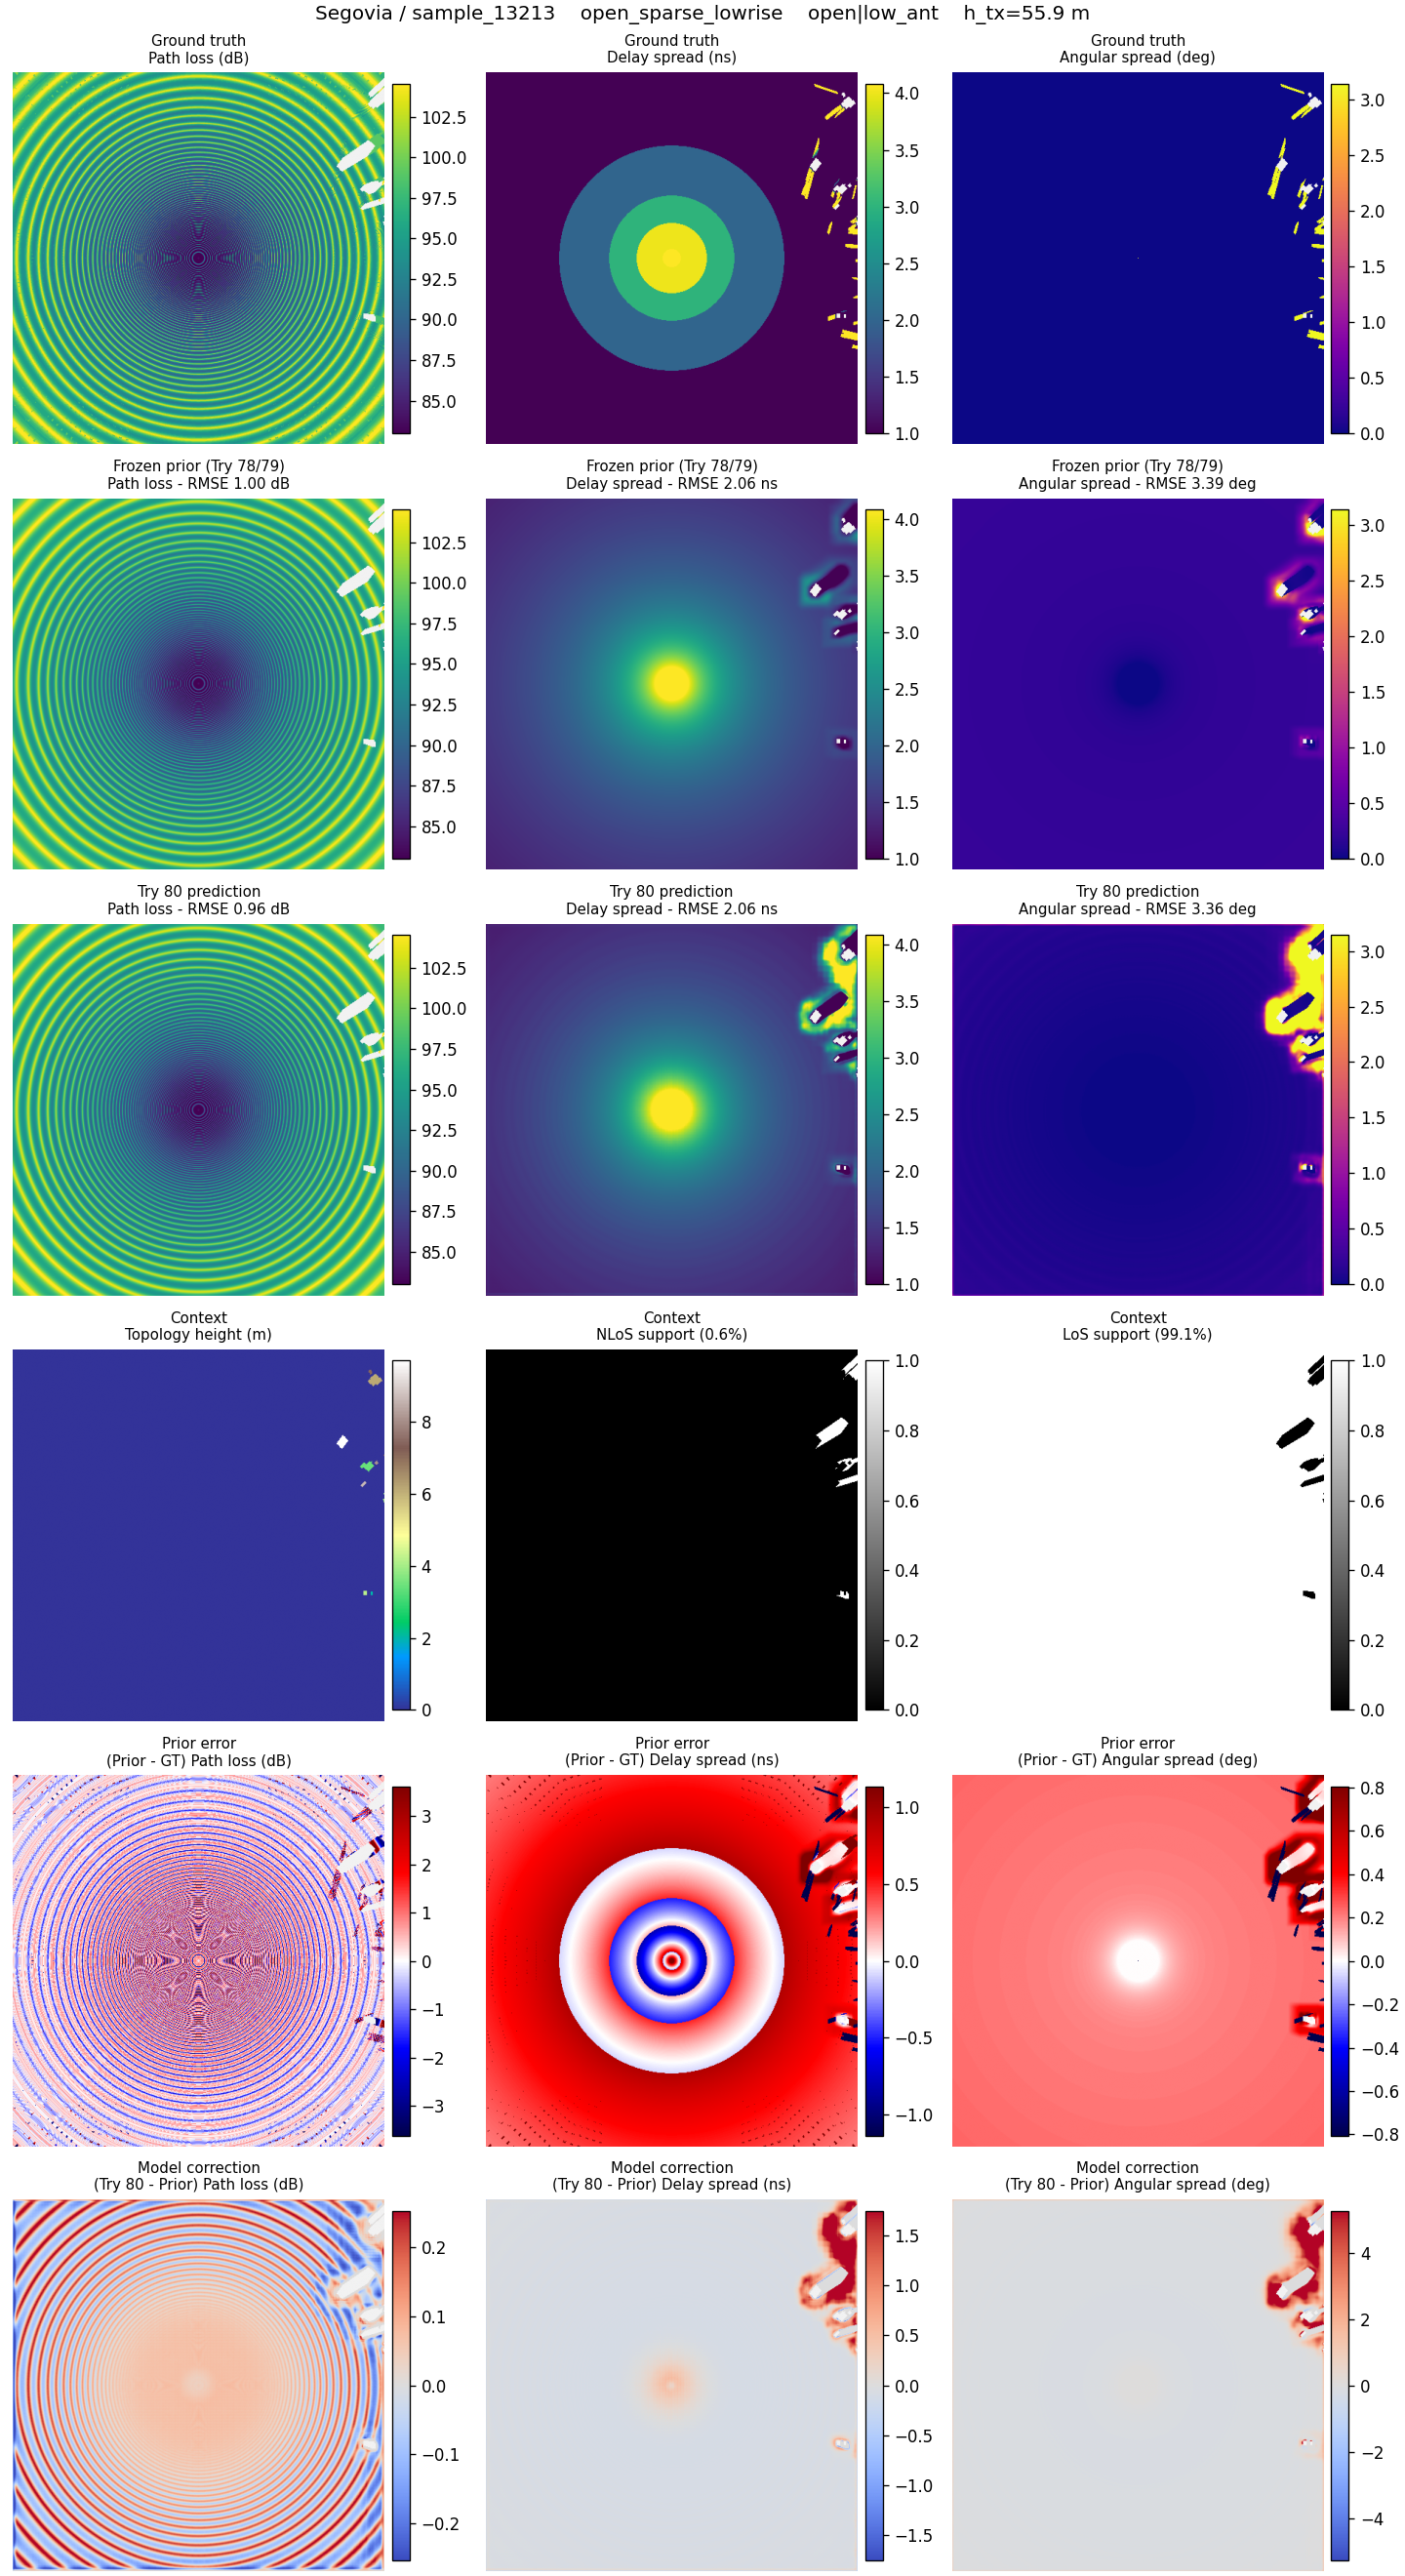
\includegraphics[width=\textwidth,height=0.88\textheight,keepaspectratio]{img/thesis_figures/try80_appendix_panels/try80_panel_open_low_ant_Segovia_sample_13213_6x3.png}
\caption{Final residual GMM-head model \(6\times3\) inspection panel for an open, low-antenna
validation sample in Segovia.}
\label{fig:appendix_try80_open_low}
\end{figure}

\clearpage
\begin{figure}[p]
\centering
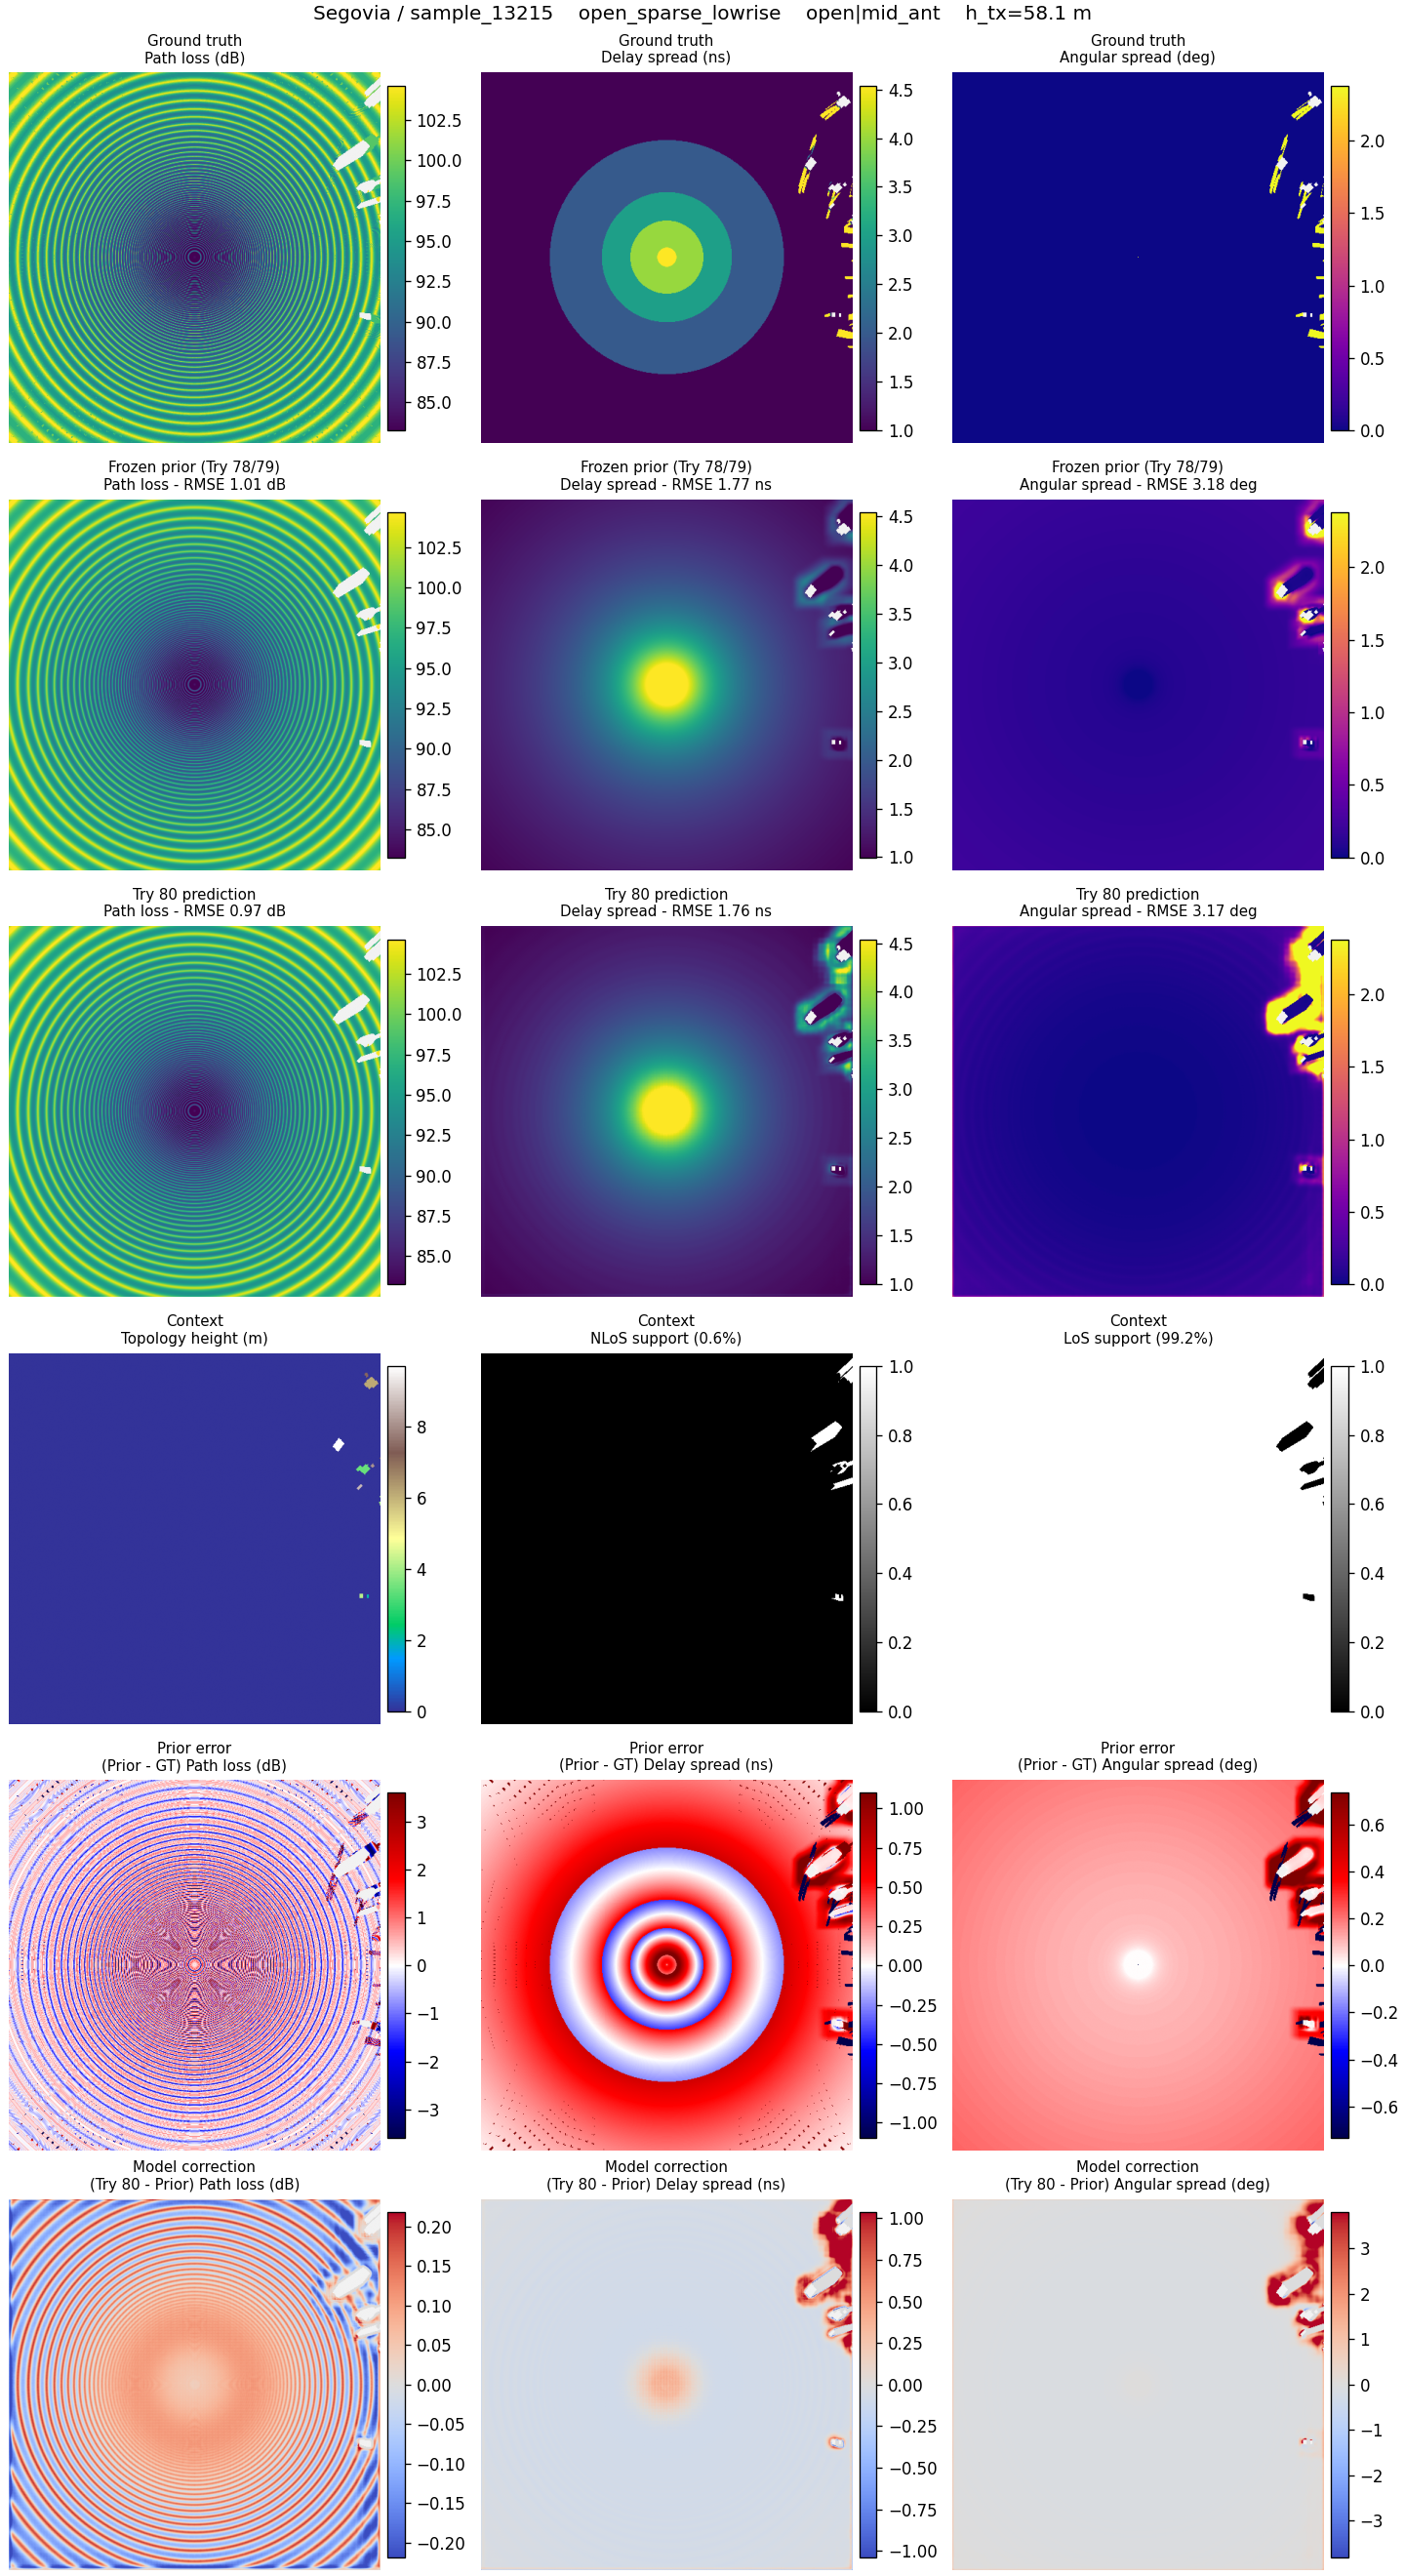
\includegraphics[width=\textwidth,height=0.88\textheight,keepaspectratio]{img/thesis_figures/try80_appendix_panels/try80_panel_open_mid_ant_Segovia_sample_13215_6x3.png}
\caption{Final residual GMM-head model \(6\times3\) inspection panel for an open, mid-antenna
validation sample in Segovia.}
\label{fig:appendix_try80_open_mid}
\end{figure}

\clearpage
\begin{figure}[p]
\centering
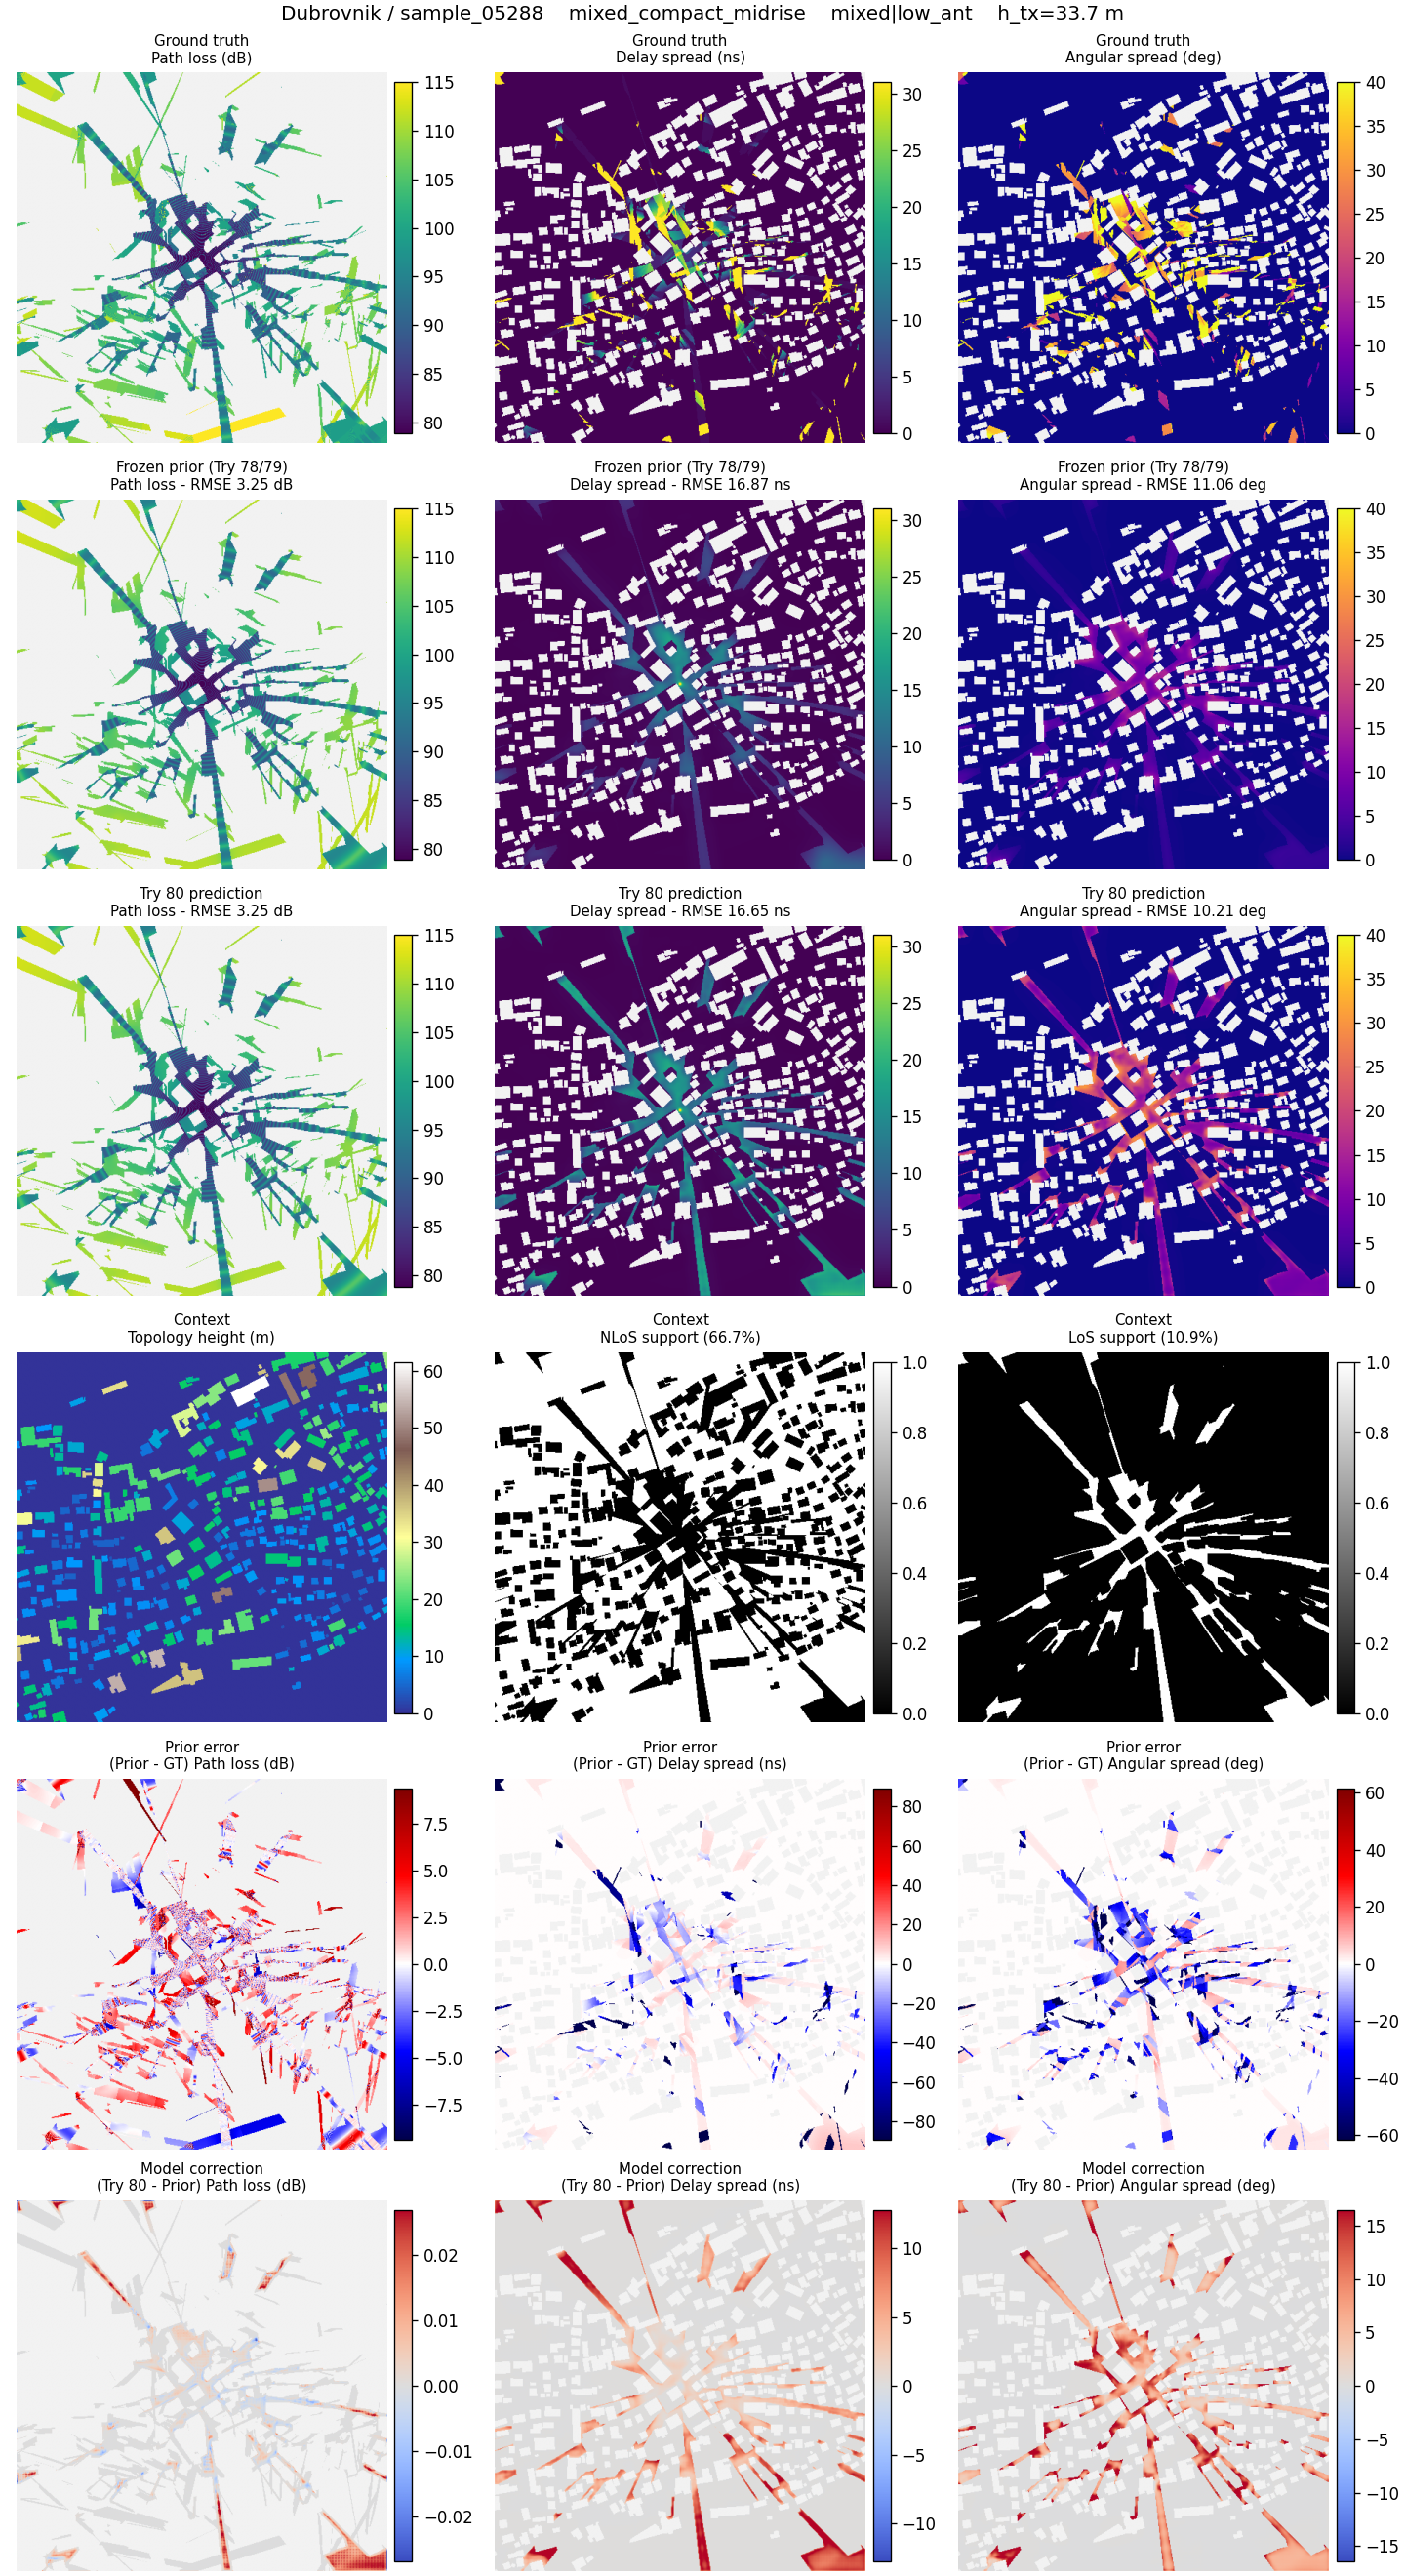
\includegraphics[width=\textwidth,height=0.88\textheight,keepaspectratio]{img/thesis_figures/try80_appendix_panels/try80_panel_mixed_low_ant_Dubrovnik_sample_05288_6x3.png}
\caption{Final residual GMM-head model \(6\times3\) inspection panel for a mixed, low-antenna
validation sample in Dubrovnik.}
\label{fig:appendix_try80_mixed_low}
\end{figure}

\clearpage
\begin{figure}[p]
\centering
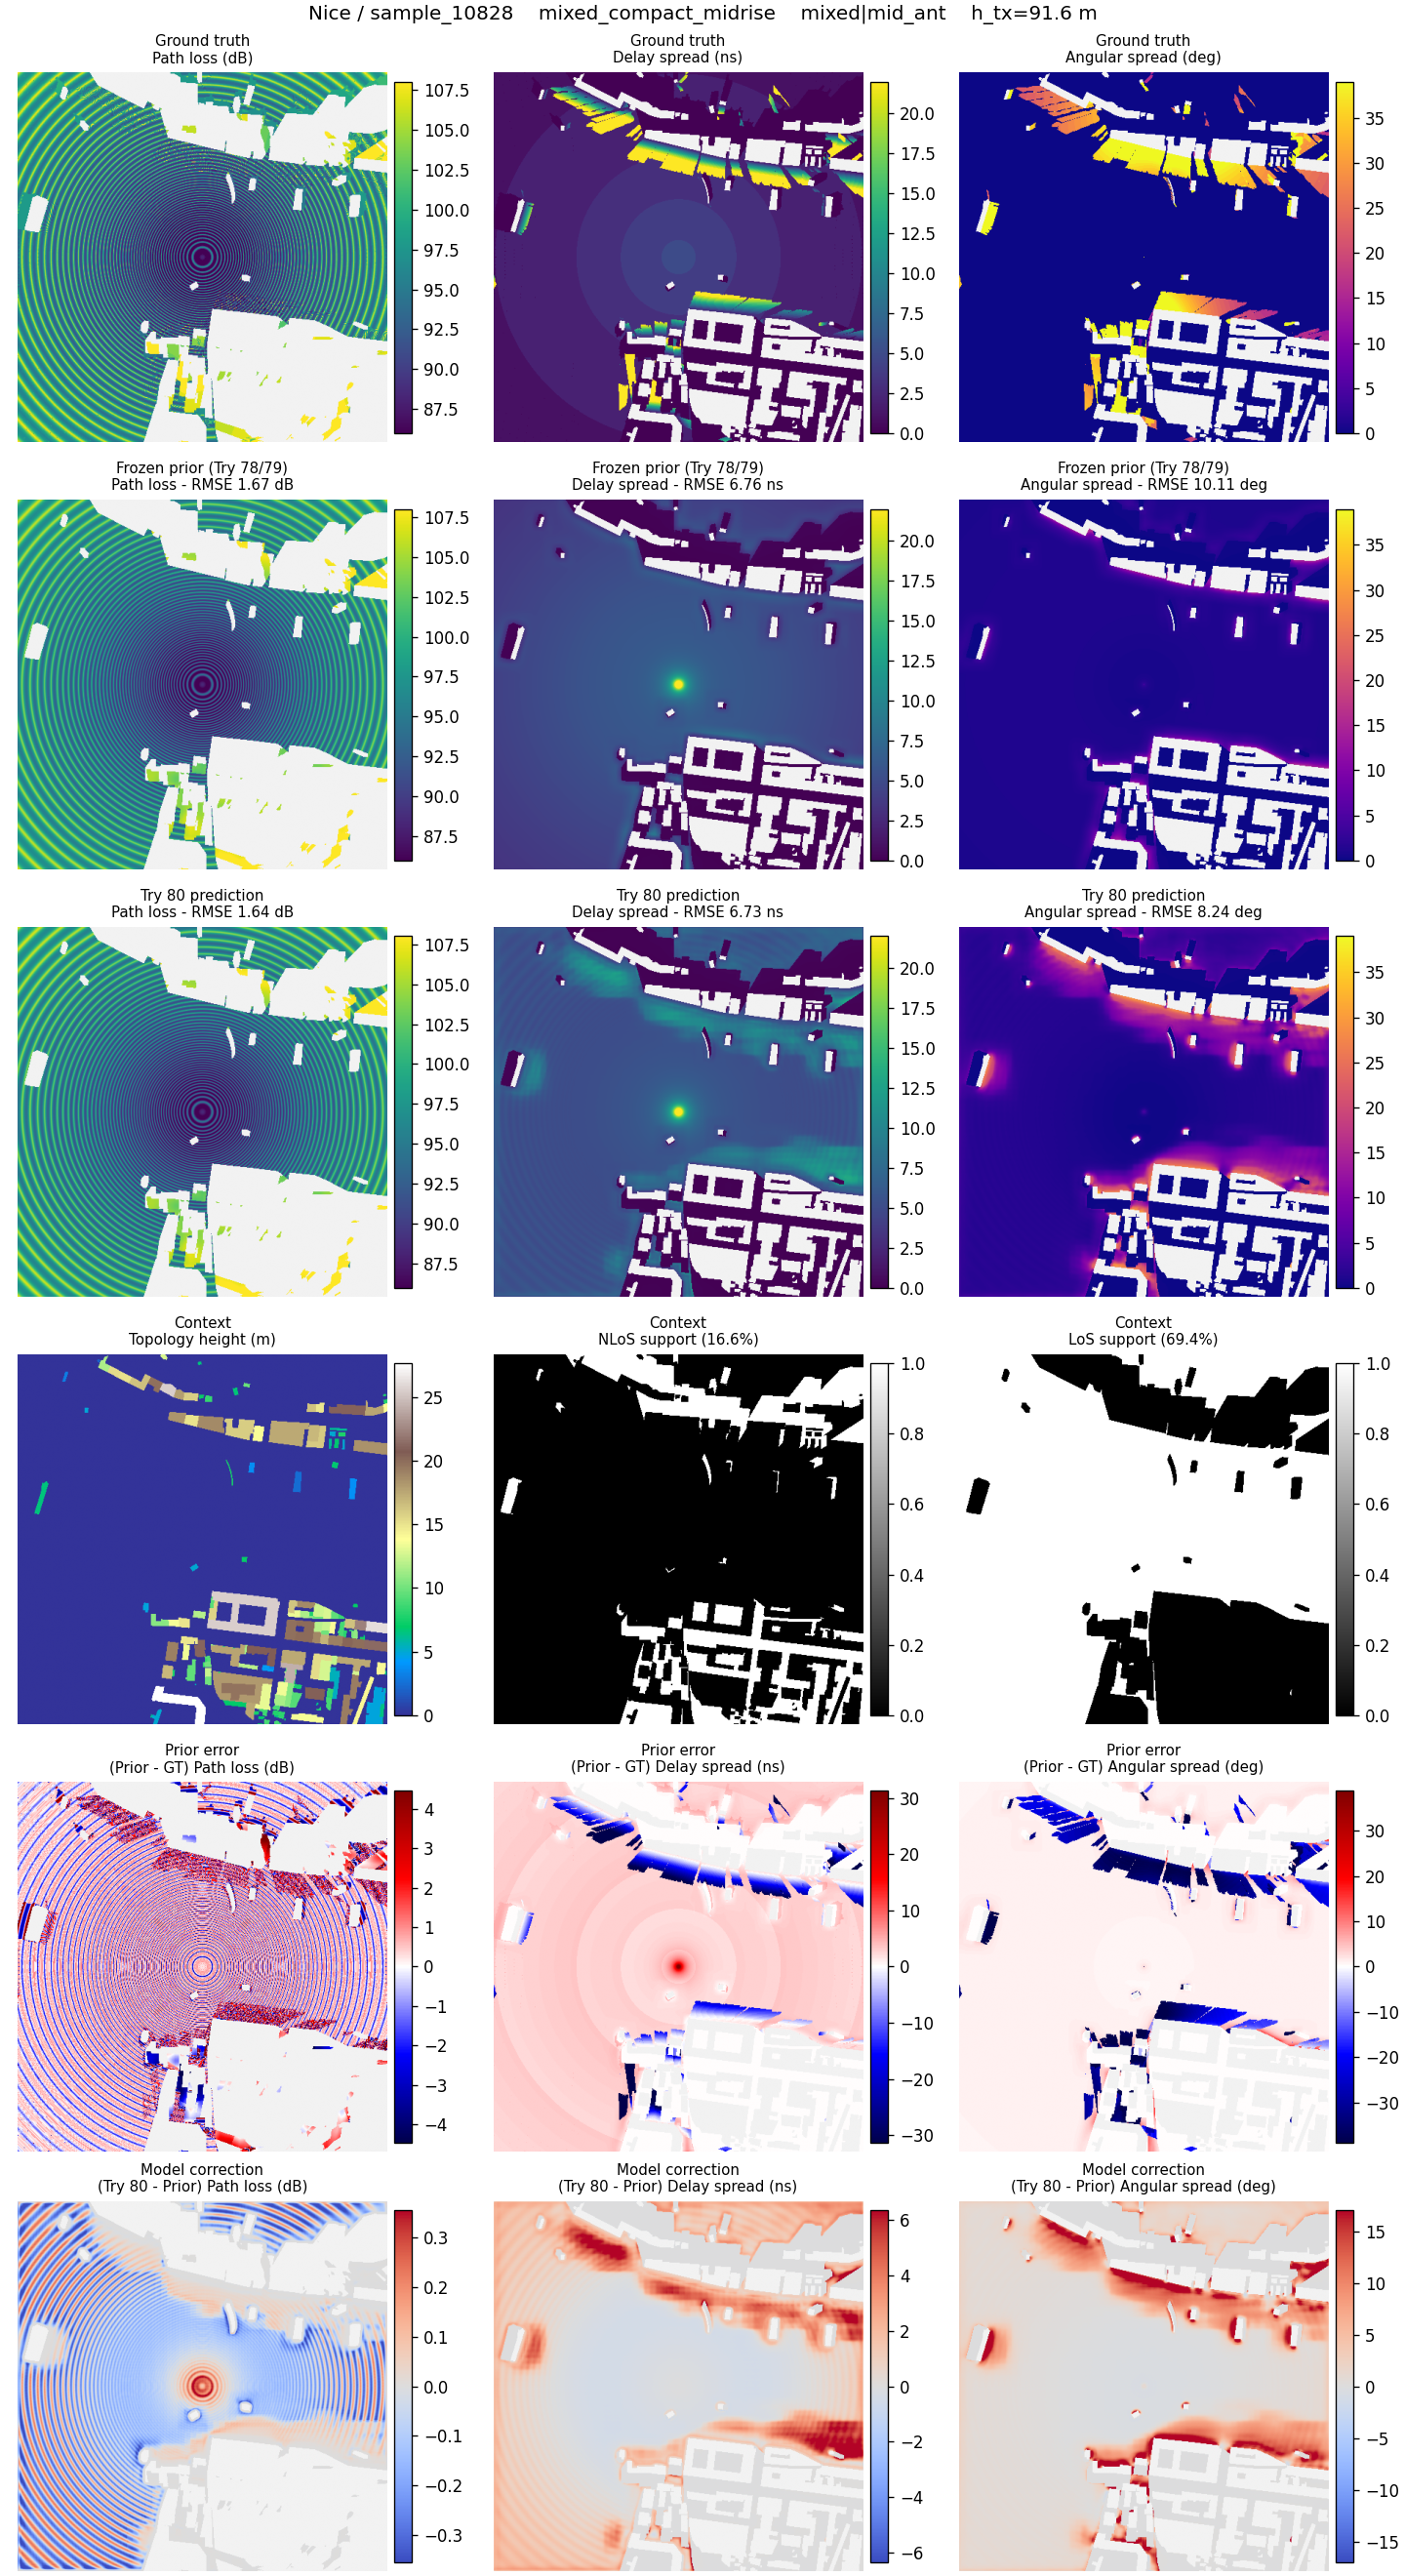
\includegraphics[width=\textwidth,height=0.88\textheight,keepaspectratio]{img/thesis_figures/try80_appendix_panels/try80_panel_mixed_mid_ant_Nice_sample_10828_6x3.png}
\caption{Final residual GMM-head model \(6\times3\) inspection panel for a mixed, mid-antenna
validation sample in Nice.}
\label{fig:appendix_try80_mixed_mid}
\end{figure}

\clearpage
\begin{figure}[p]
\centering
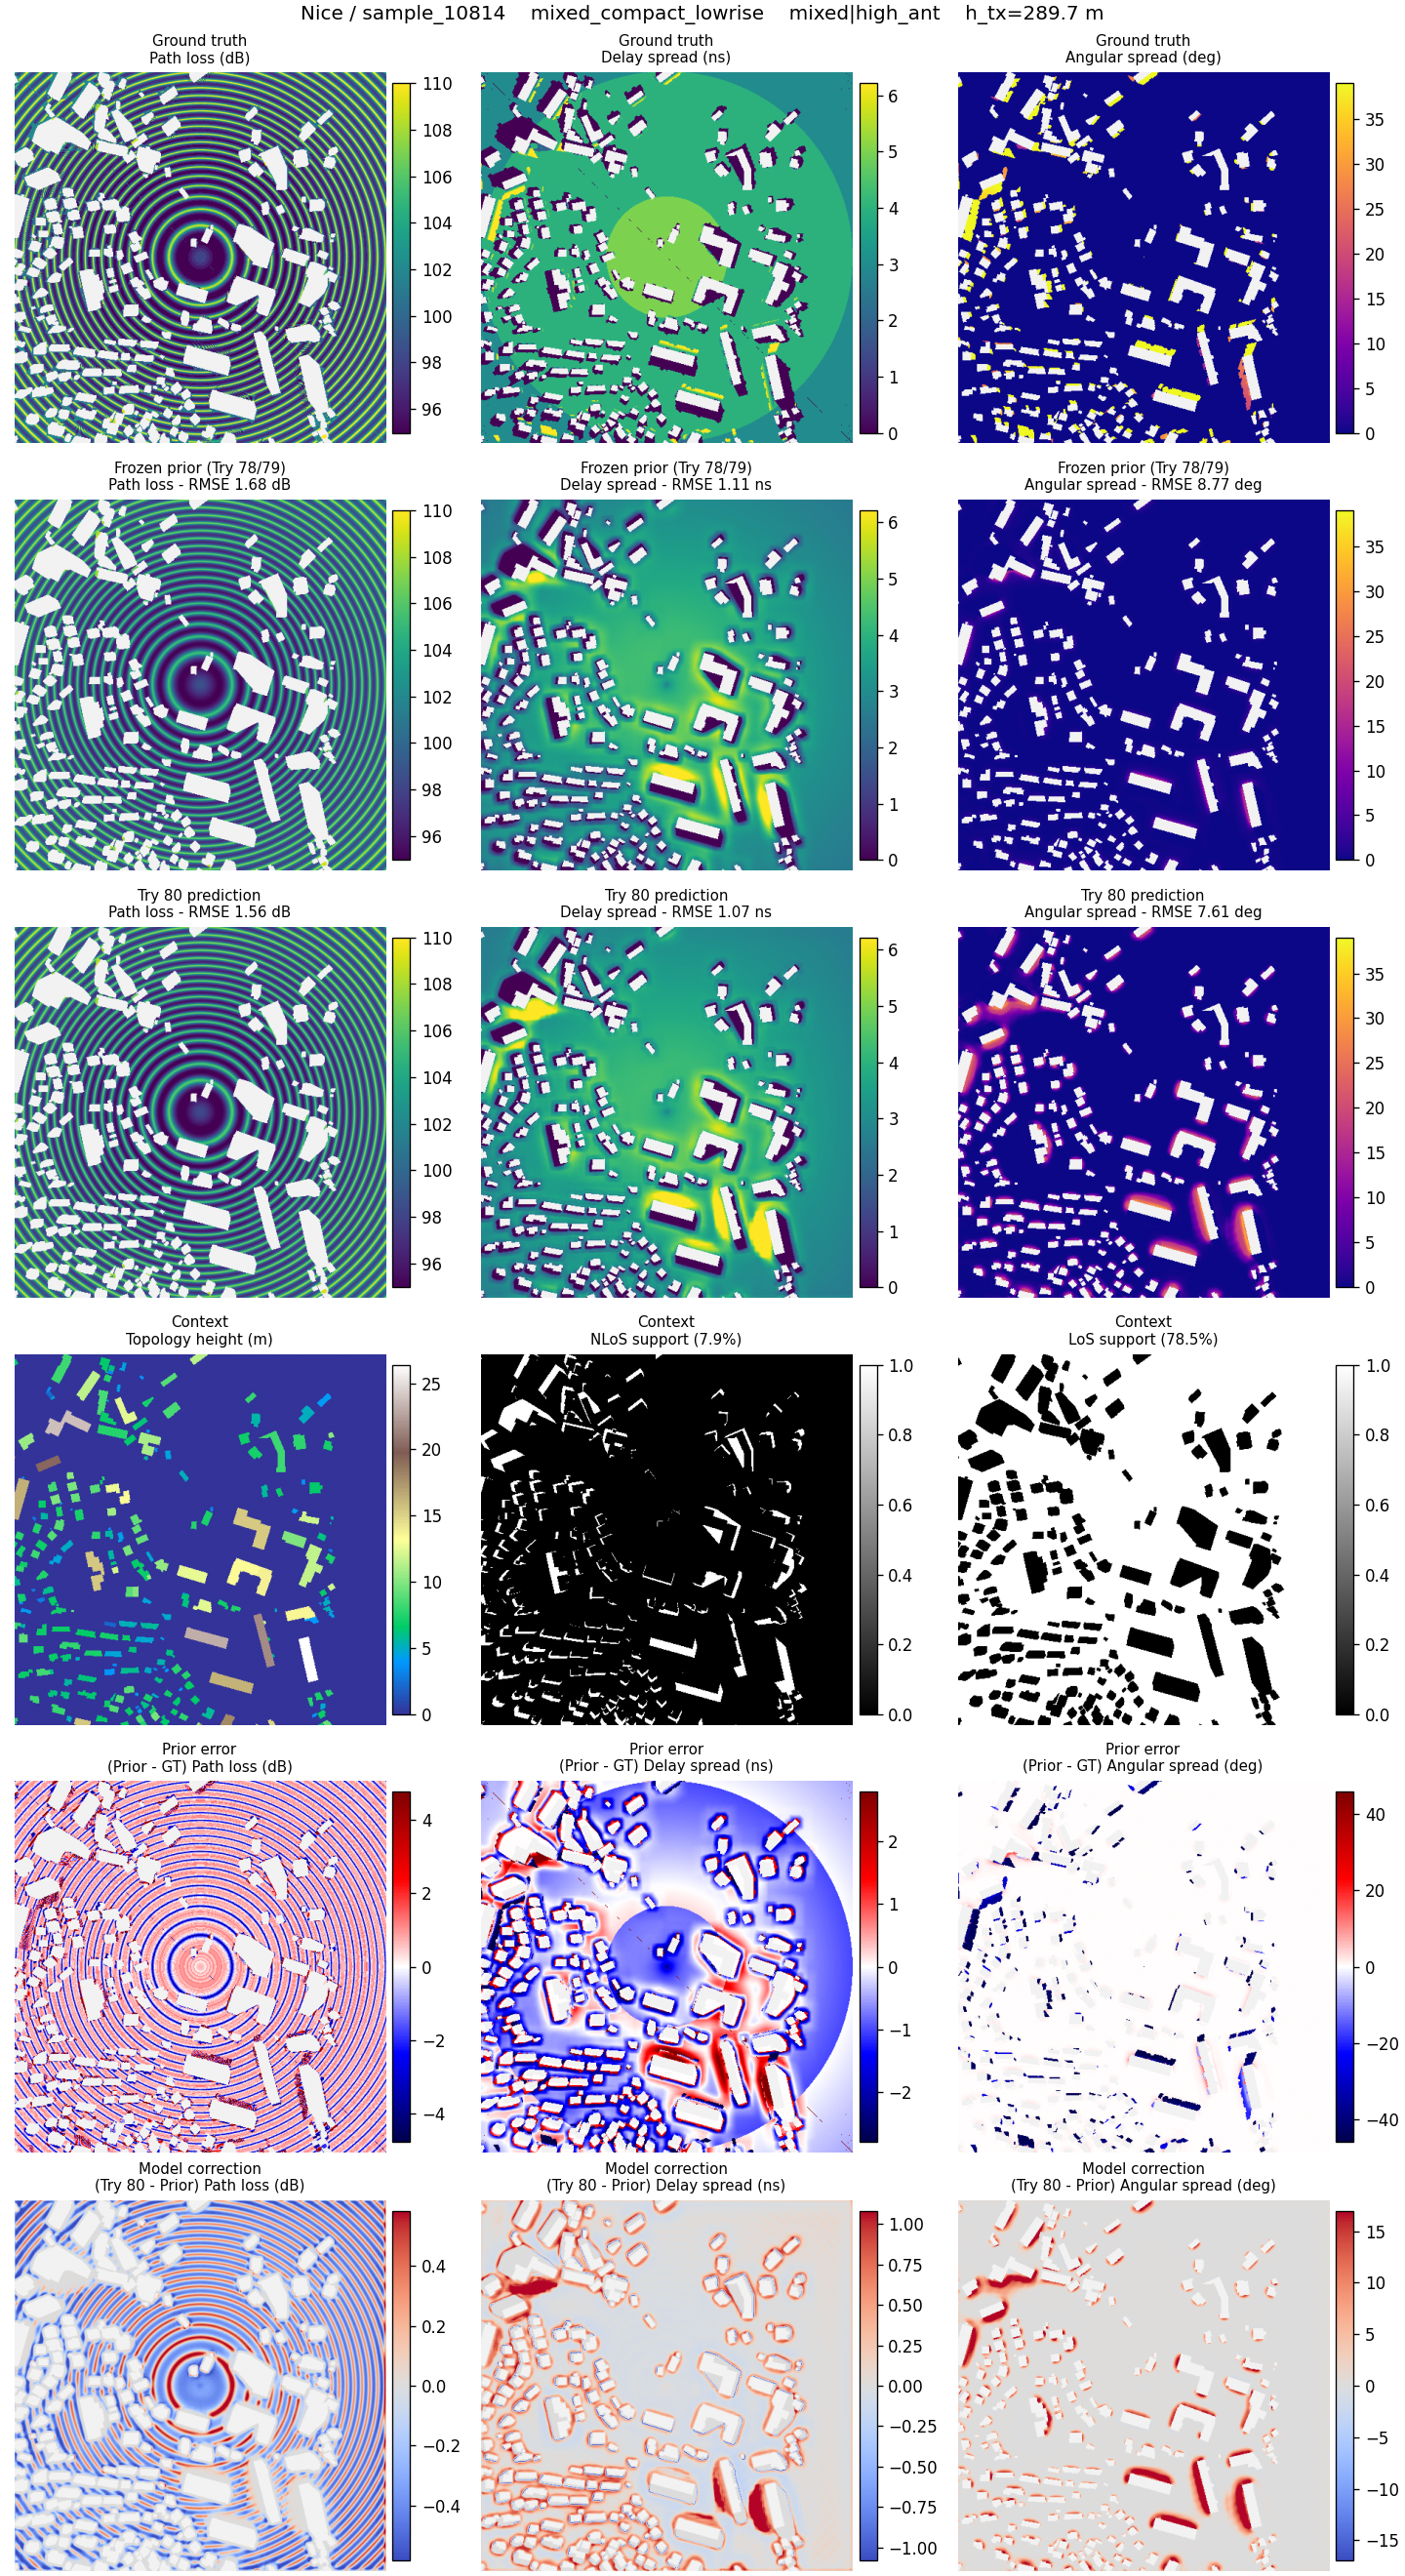
\includegraphics[width=\textwidth,height=0.88\textheight,keepaspectratio]{img/thesis_figures/try80_appendix_panels/try80_panel_mixed_high_ant_Nice_sample_10814_6x3.png}
\caption{Final residual GMM-head model \(6\times3\) inspection panel for a mixed, high-antenna
validation sample in Nice.}
\label{fig:appendix_try80_mixed_high}
\end{figure}

\clearpage
\begin{figure}[p]
\centering
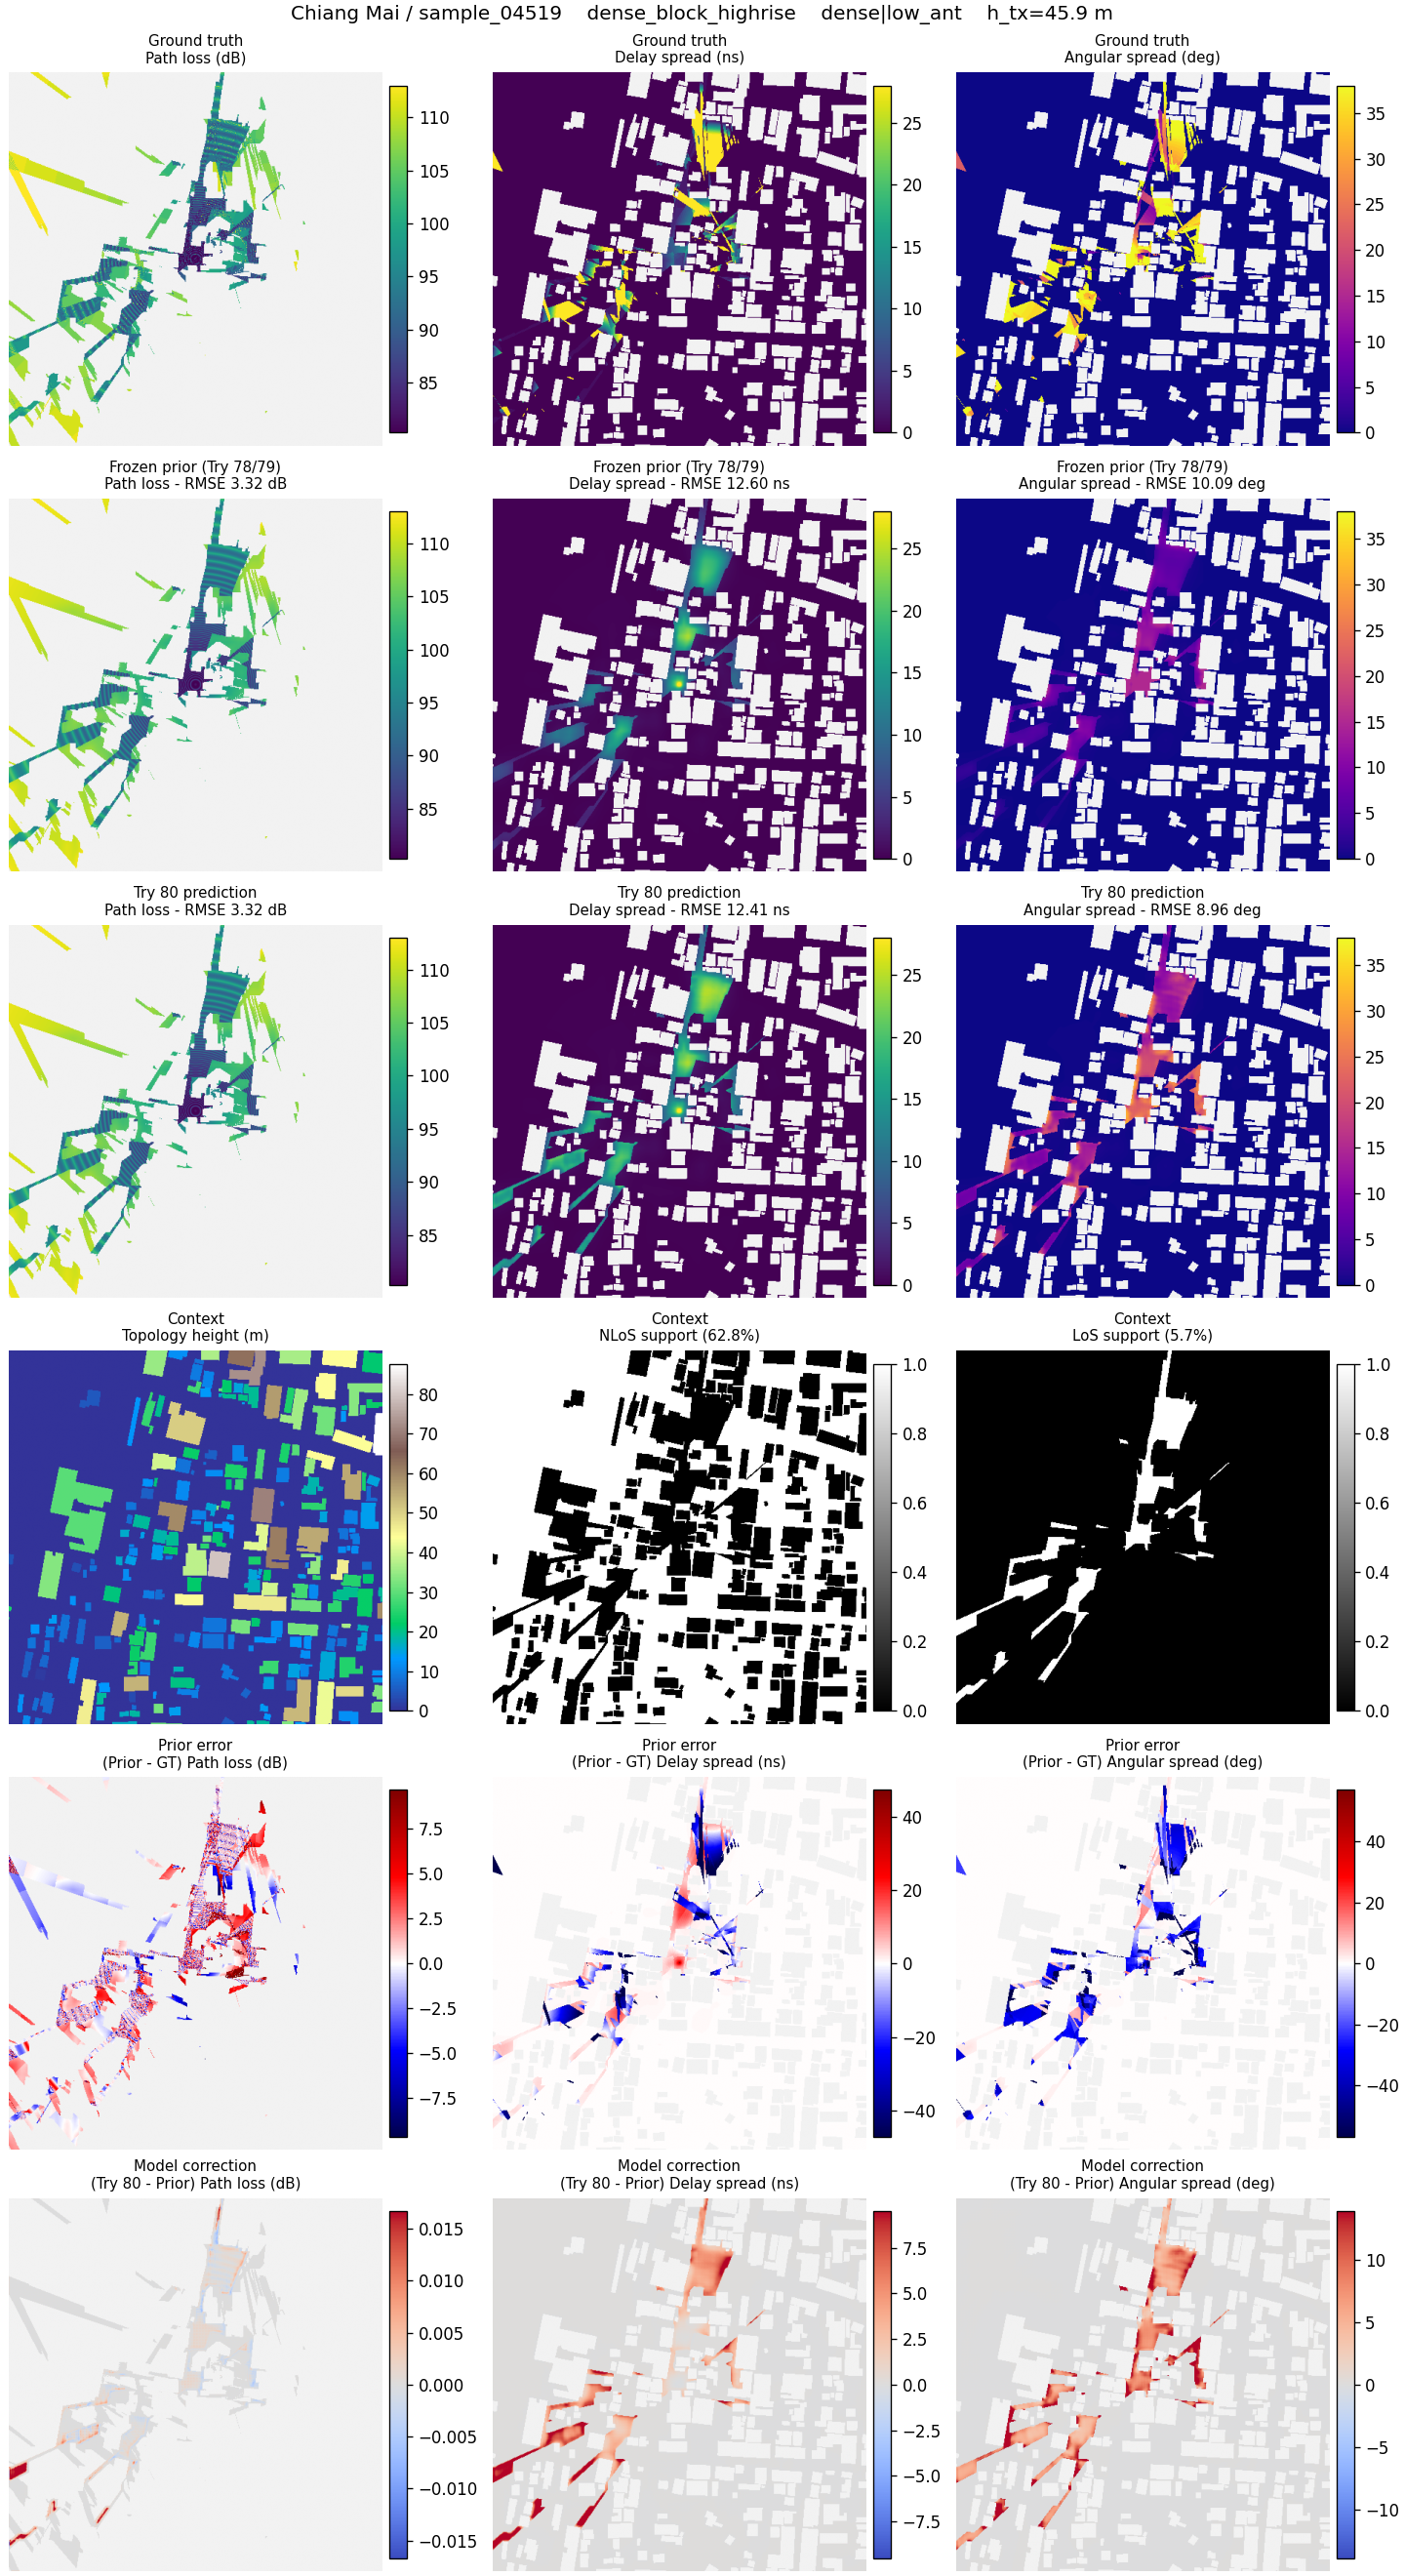
\includegraphics[width=\textwidth,height=0.88\textheight,keepaspectratio]{img/thesis_figures/try80_appendix_panels/try80_panel_dense_low_ant_Chiang_Mai_sample_04519_6x3.png}
\caption{Final residual GMM-head model \(6\times3\) inspection panel for a dense, low-antenna
validation sample in Chiang Mai.}
\label{fig:appendix_try80_dense_low}
\end{figure}

\clearpage
\begin{figure}[p]
\centering
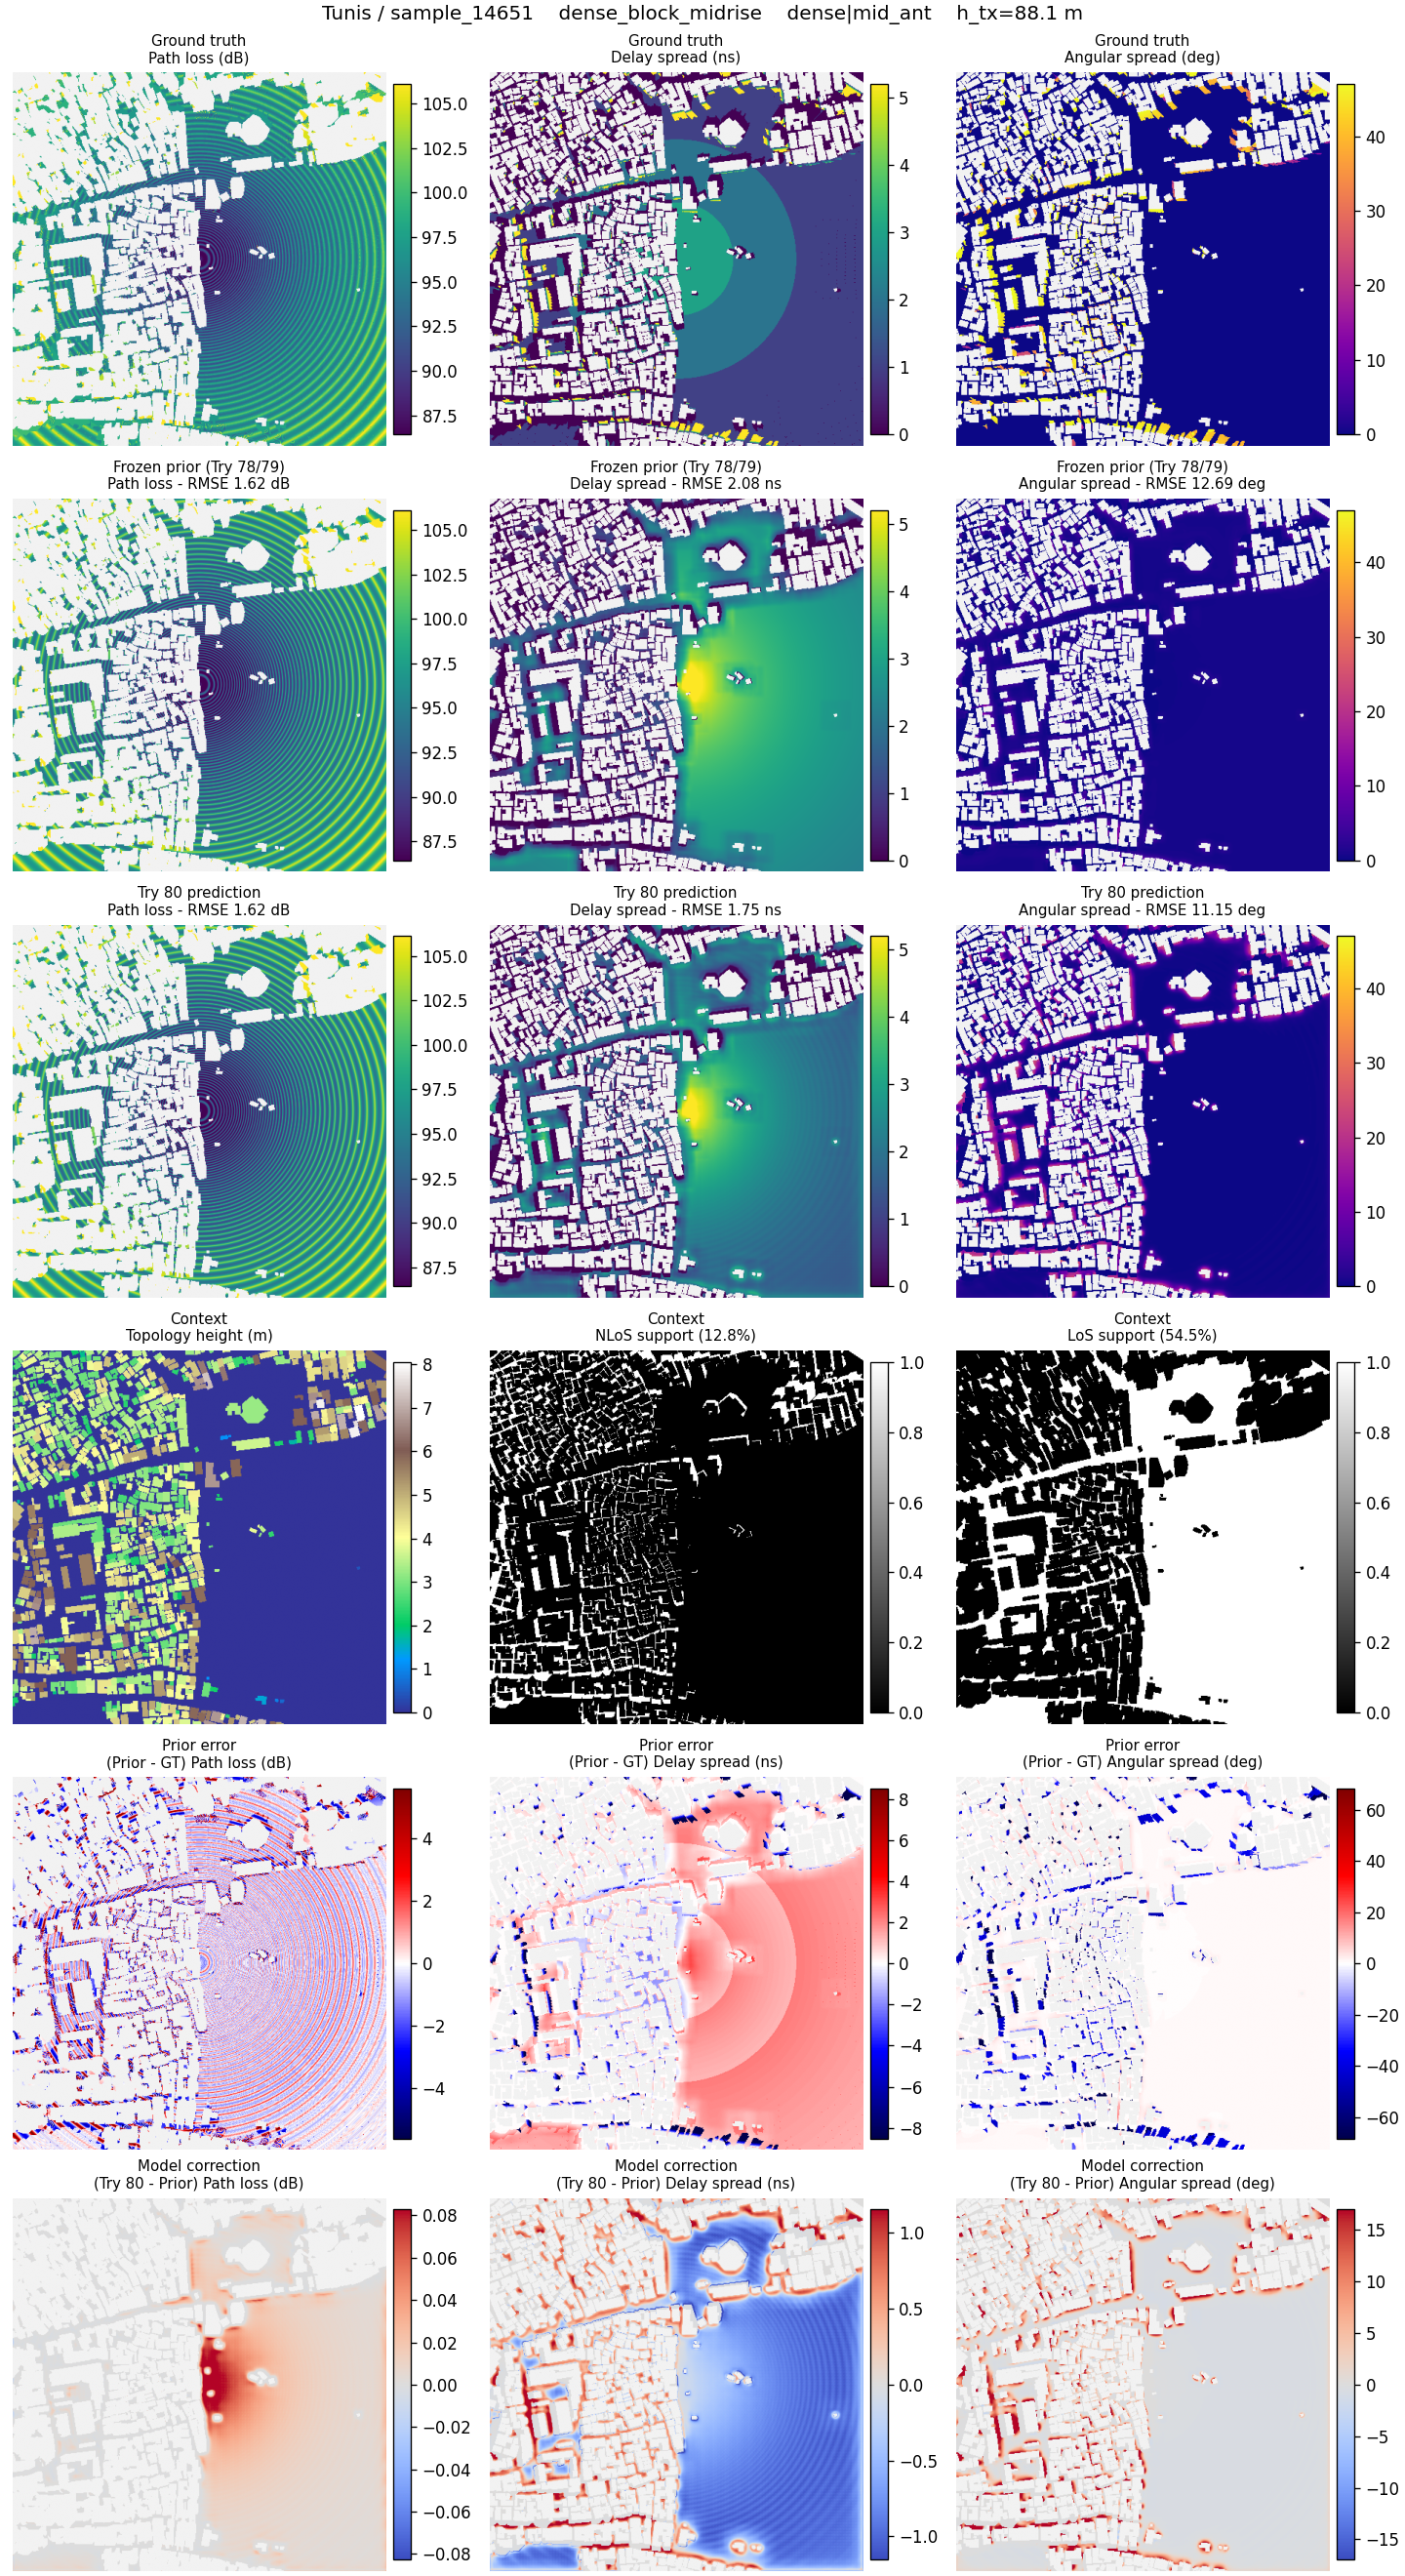
\includegraphics[width=\textwidth,height=0.88\textheight,keepaspectratio]{img/thesis_figures/try80_appendix_panels/try80_panel_dense_mid_ant_Tunis_sample_14651_6x3.png}
\caption{Final residual GMM-head model \(6\times3\) inspection panel for a dense, mid-antenna
validation sample in Tunis.}
\label{fig:appendix_try80_dense_mid}
\end{figure}

\clearpage
\begin{figure}[p]
\centering
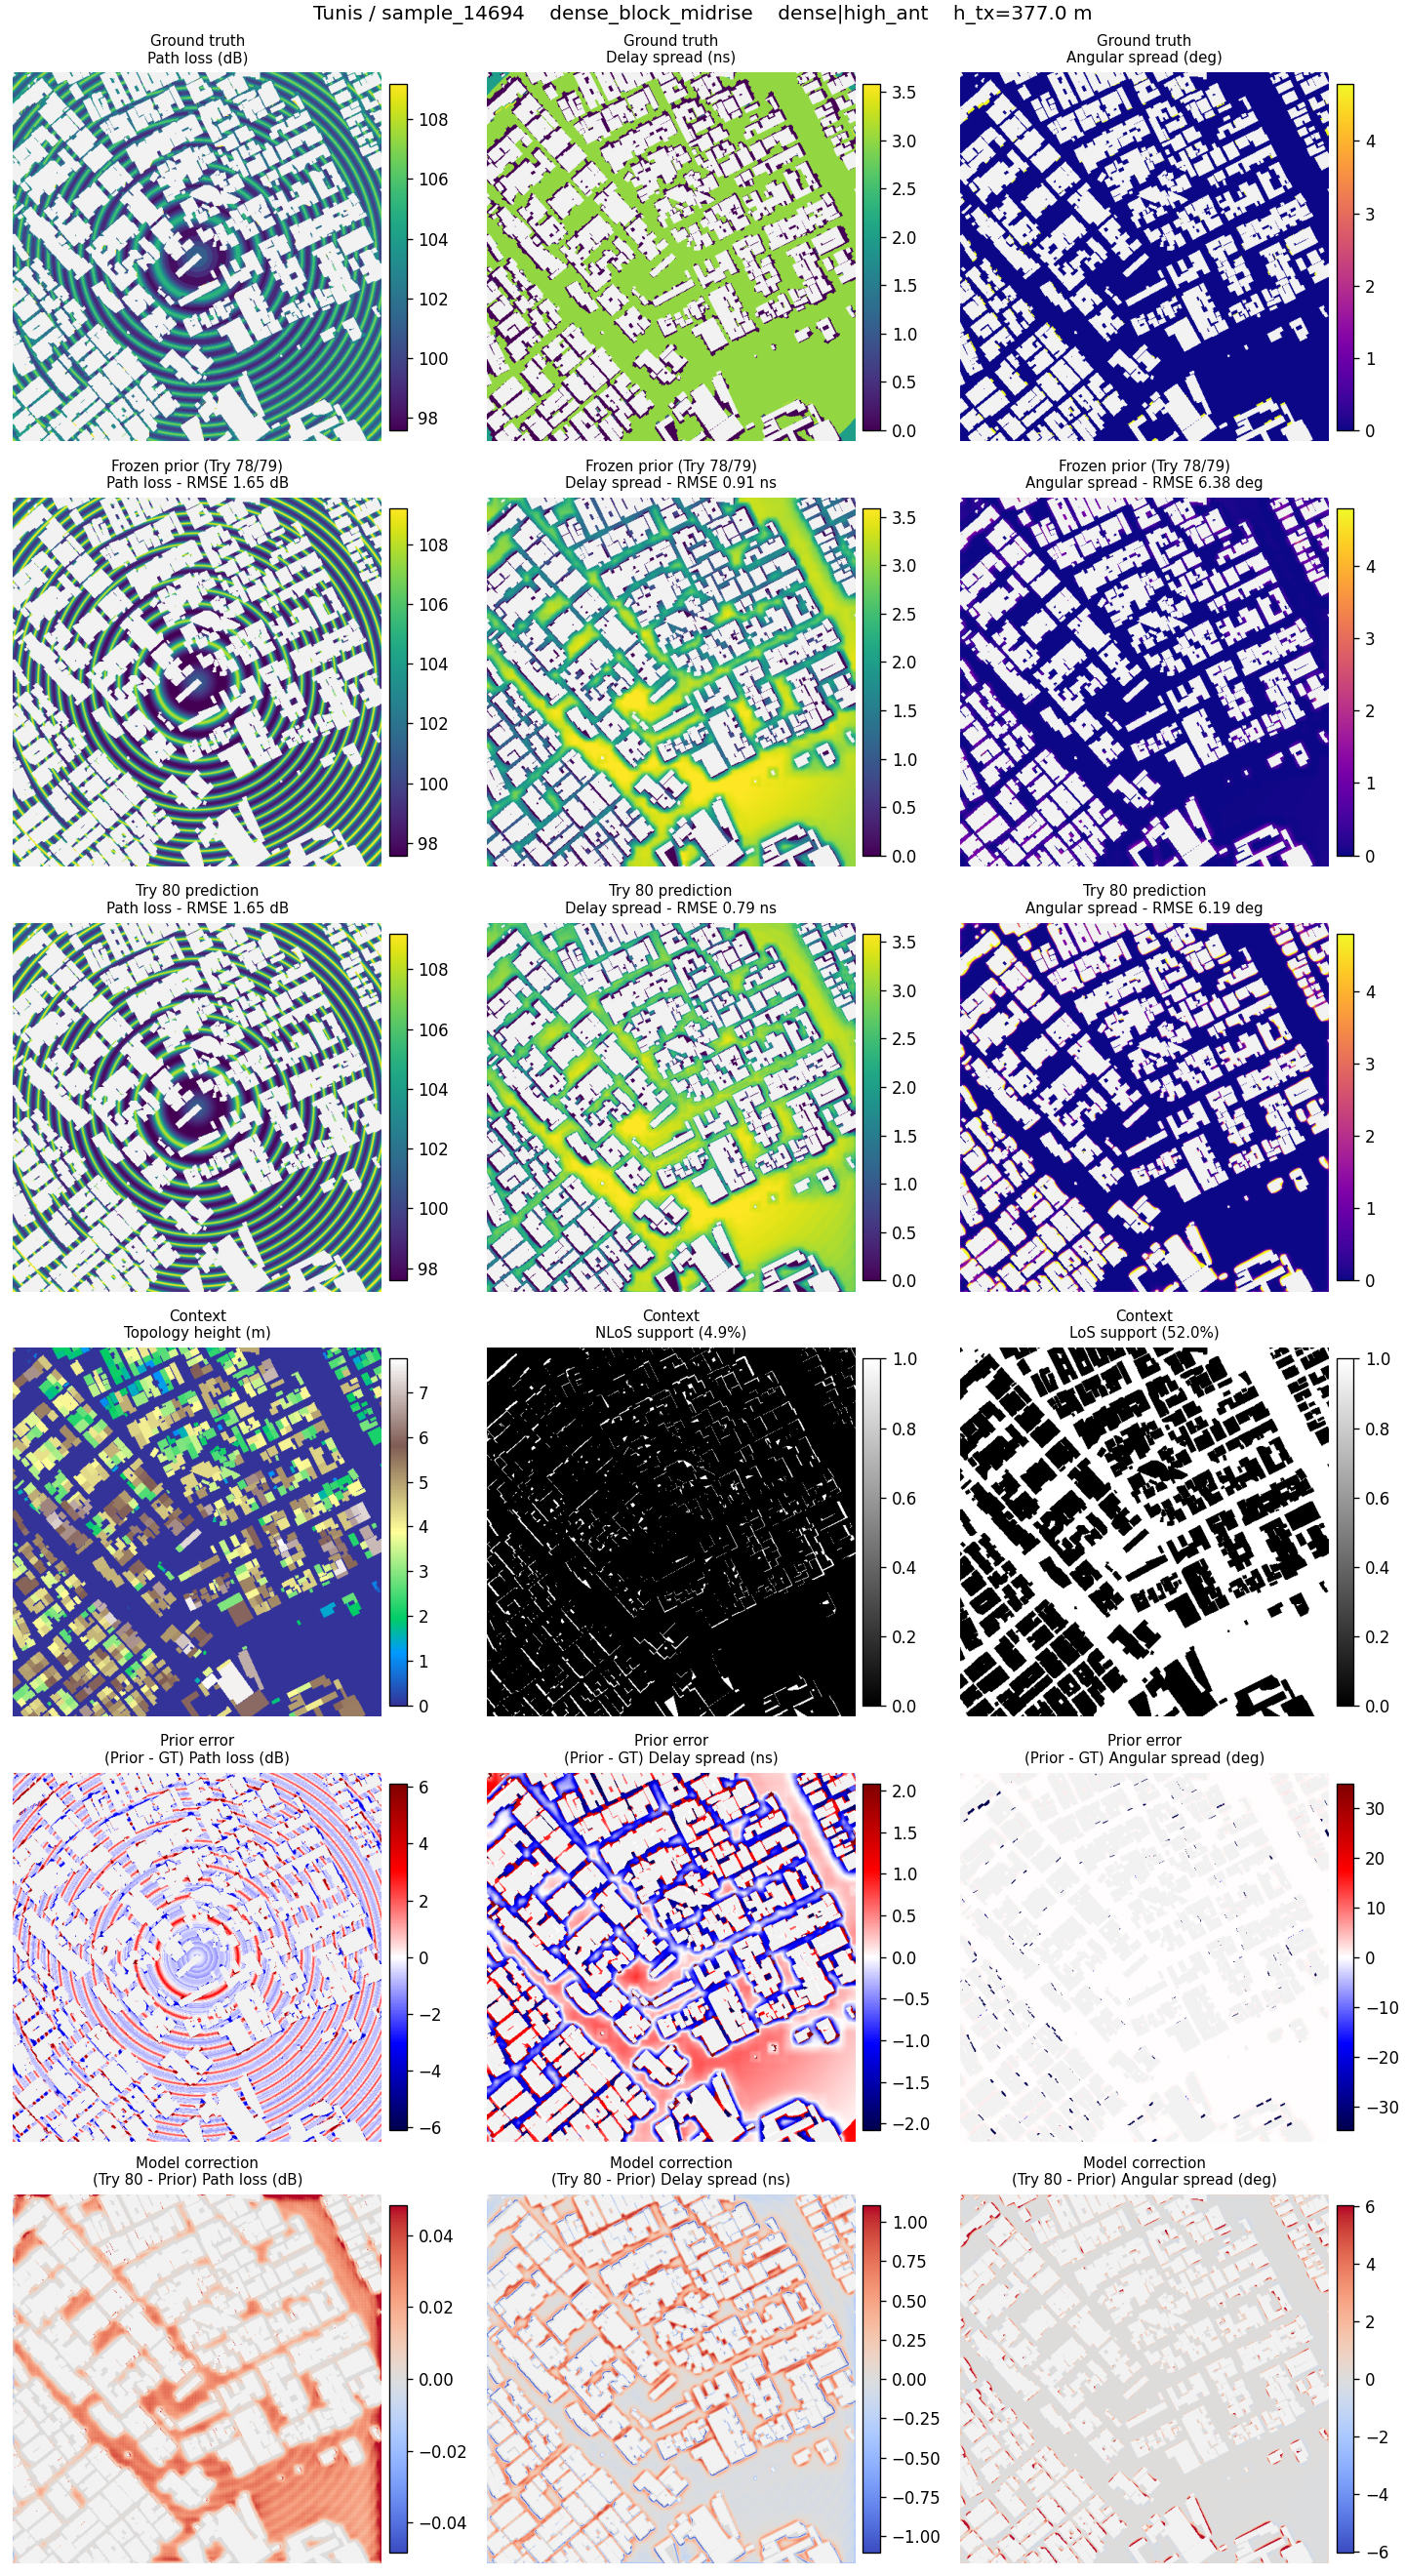
\includegraphics[width=\textwidth,height=0.88\textheight,keepaspectratio]{img/thesis_figures/try80_appendix_panels/try80_panel_dense_high_ant_Tunis_sample_14694_6x3.png}
\caption{Final residual GMM-head model \(6\times3\) inspection panel for a dense, high-antenna
validation sample in Tunis.}
\label{fig:appendix_try80_dense_high}
\end{figure}

\clearpage
\chapter{CKM Generator Interface and Reproducibility Tool}
\label{chap:ckm_generator}
\label{app:ckm_generator}

This appendix documents the standalone CKM Generator delivered with the final
residual GMM-head pipeline. The tool was built to make the trained model usable outside
the training scripts: it accepts topology inputs, prepares them with the same
geometric conventions used in the thesis, computes or imports LoS/NLoS masks,
evaluates the frozen calibrated priors, optionally runs the final neural model,
and exports the numerical arrays used for reproducible analysis. It can also
export visual figures when those optional inspection switches are enabled.

The generator is intentionally available through two front ends. The Streamlit
application is designed for inspection, rapid manual testing, and demonstrations
with uploaded files. The command-line interface uses the same backend and is
intended for reproducible scripted runs, validation, and larger batches.

\section{Public source record and checkpoint artifact}

The reproducibility record is split across public repositories. The standalone
generator is maintained in \texttt{CKMGenerator}; the final training and
evaluation code is collected in \texttt{Final\_Code\_TFG}; the broader
experimental history is preserved in
\texttt{TFGAllProgress\_Tries\_and\_Attempts}; and the thesis source is kept in
\texttt{TFG\_ActualText\_LaTeX}
\cite{moreno2026ckmgenerator,moreno2026finalcode,moreno2026tfgprogress,moreno2026tfgtext}.

The final checkpoint loaded by the generator is
\texttt{models/best\_model.pt}. Since this file is larger than GitHub's regular
single-file limit for ordinary Git history, it is treated as a large model
artifact rather than normal source code. The generator therefore accepts either
the local default checkpoint path or an explicit \texttt{--checkpoint} path,
while the public source repository remains small enough to clone and inspect
normally.

\section{Interface overview}

Figure~\ref{fig:ckm_generator_controls} shows the main controls exposed by the
Streamlit interface. The left sidebar controls the input source, antenna height,
runtime device, mask policy, model execution, export format, image scaling,
pixel spacing, HDF5 filtering, and output folder.

\begin{figure}[H]
\centering

\includegraphics[width=\textwidth,height=0.72\textheight,keepaspectratio]{img/thesis_figures/ckm_generator/ckm_generator_app_controls.png}
\caption[CKM Generator Streamlit interface.]%
{CKM Generator Streamlit interface. The sidebar exposes the same
settings that are available through the command-line interface.}
\label{fig:ckm_generator_controls}
\end{figure}

After generation, the application presents the fitted topology next to the
LoS and NLoS masks actually used by the priors and model. This is important
because the masks are not only visual outputs: they are part of the final model
input tensor and determine the receiver-valid support used by the priors.
Figure~\ref{fig:ckm_generator_masks} shows this inspection view.

\begin{figure}[H]
\centering
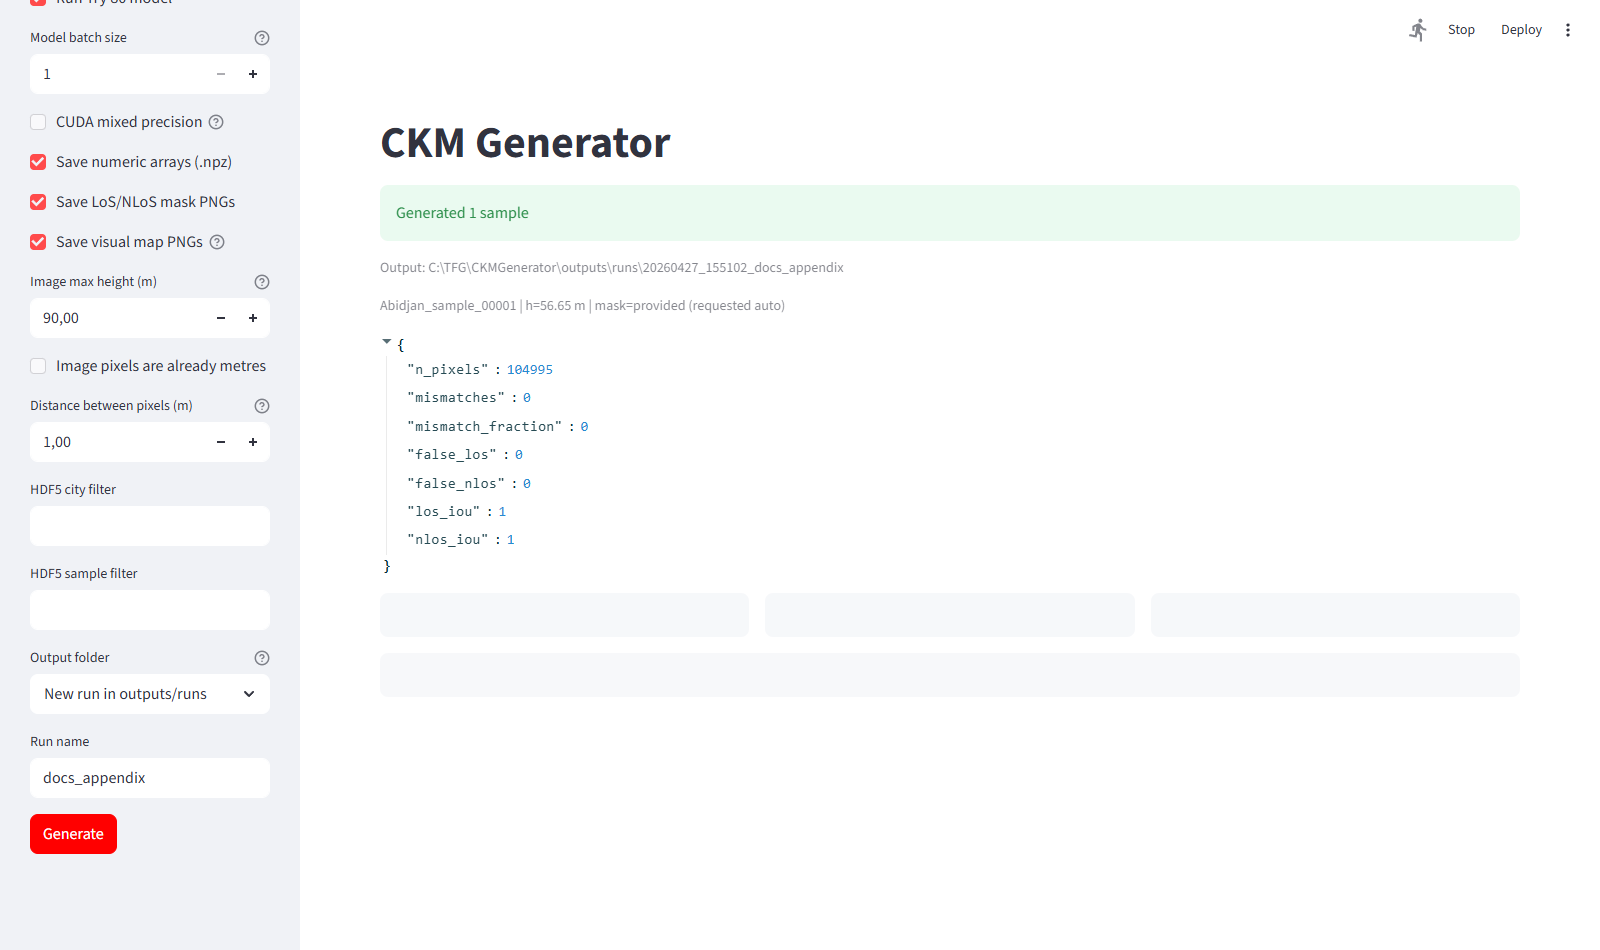
\includegraphics[width=\textwidth,height=0.72\textheight,keepaspectratio]{img/thesis_figures/ckm_generator/ckm_generator_app_result_top.png}
\caption[Generated topology and masks.]%
{Generated topology and masks for an HDF5 sample. The view reports
the resolved mask source and displays topology, LoS mask, and NLoS mask
side by side.}
\label{fig:ckm_generator_masks}
\end{figure}

When the final model is enabled, the generator produces the three target
maps in their native units. Figure~\ref{fig:ckm_generator_prediction} shows
the joint prediction panel saved by the tool.

\begin{figure}[H]
\centering
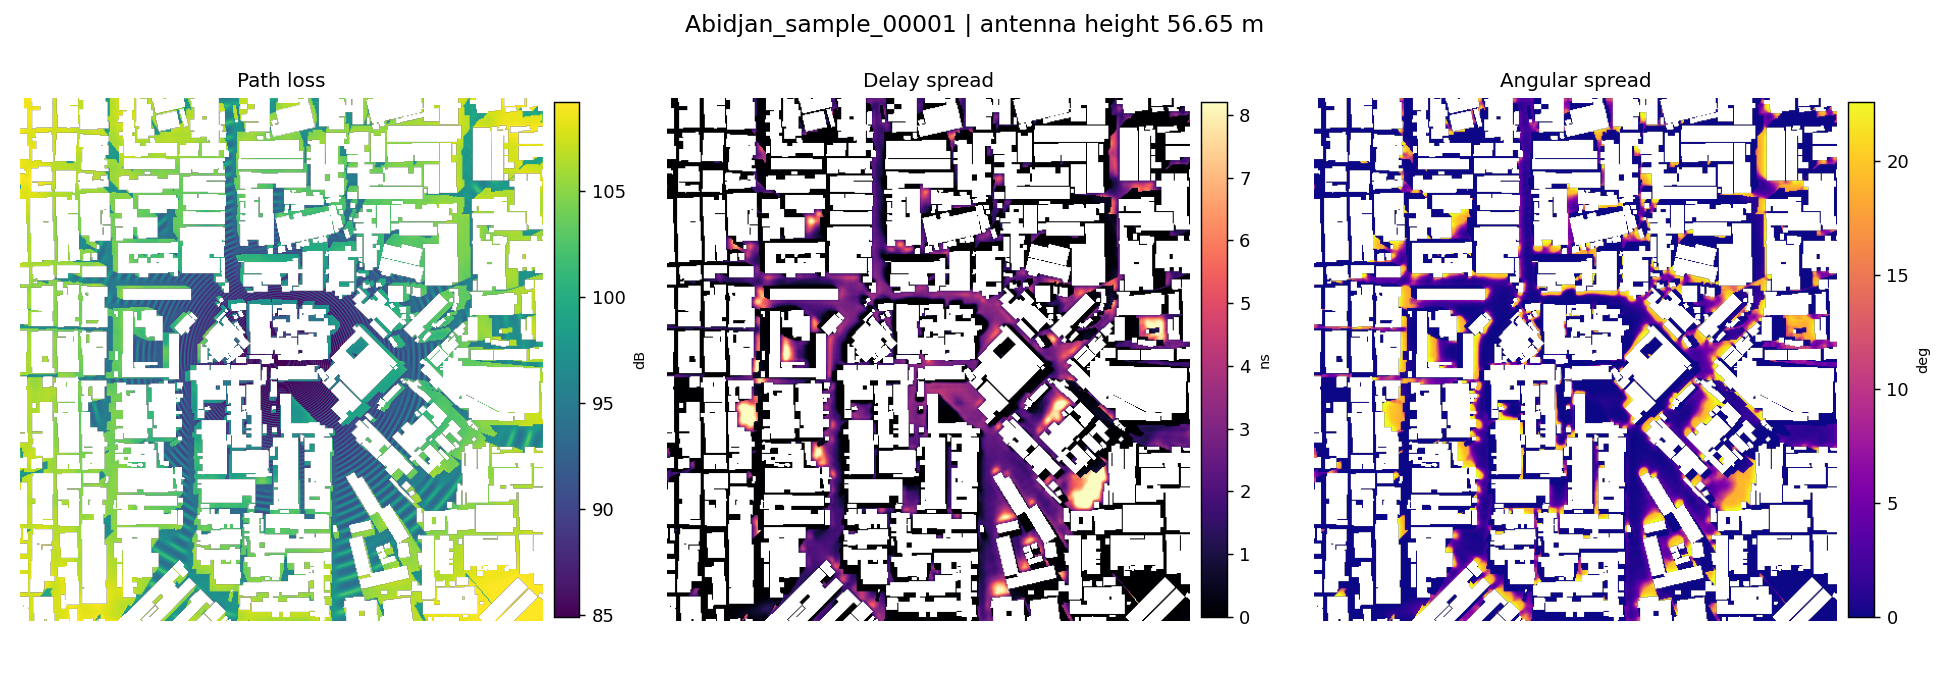
\includegraphics[width=\textwidth,height=0.72\textheight,keepaspectratio]{img/thesis_figures/ckm_generator/ckm_generator_prediction_joint.png}
\caption[CKM Generator joint prediction output.]%
{Joint prediction figure exported by the CKM Generator, with path
loss in dB, delay spread in ns, and angular spread in degrees.}
\label{fig:ckm_generator_prediction}
\end{figure}

\section{How the tool is run}

The dependencies are installed in the Python environment that will run the
tool:

{\scriptsize
\begin{verbatim}
cd C:\TFG\CKMGenerator
C:\Python310\python.exe -m pip install -r C:\TFG\CKMGenerator\requirements.txt
\end{verbatim}
}

The runtime check is executed before inference:

{\scriptsize
\begin{verbatim}
C:\Python310\python.exe C:\TFG\CKMGenerator\ckm_doctor.py
\end{verbatim}
}

The doctor command checks PyTorch, CUDA, DirectML, the checkpoint, available
memory, and whether the selected runtime can execute the final model. In
\texttt{auto} mode, the runtime priority is CUDA, then DirectML, then CPU.

The Streamlit application is started with:

{\scriptsize
\begin{verbatim}
C:\Python310\python.exe -m streamlit run C:\TFG\CKMGenerator\ckm_app.py
\end{verbatim}
}

The equivalent terminal command for an HDF5 sample is:

{\scriptsize
\begin{verbatim}
C:\Python310\python.exe C:\TFG\CKMGenerator\ckm_generate.py ^
  --input C:\TFG\CKMGenerator\inputs\samples\Abidjan_sample_00001.h5 ^
  --run-name abidjan_check ^
  --mixed-precision
\end{verbatim}
}

For an image-only topology, the transmitter height must be supplied explicitly
unless it is stored in a structured input file:

{\scriptsize
\begin{verbatim}
C:\Python310\python.exe C:\TFG\CKMGenerator\ckm_generate.py ^
  --input C:\path\topology_map.png ^
  --height 56.65 ^
  --topology-max-m 120 ^
  --meters-per-pixel 1.0 ^
  --mask-source auto ^
  --mixed-precision
\end{verbatim}
}

\section{Accepted inputs}

The generator accepts three families of input files:

\begin{itemize}
\setlength\itemsep{0.15em}
  \item Raster topology images: \texttt{.png}, \texttt{.jpg},
        \texttt{.jpeg}, \texttt{.tif}, \texttt{.tiff}, and \texttt{.bmp}.
  \item Numeric arrays: \texttt{.npy}, \texttt{.npz}, \texttt{.csv},
        \texttt{.txt}, and \texttt{.json}.
  \item HDF5 files: \texttt{.h5}, \texttt{.hdf5}, and \texttt{.hdf}.
\end{itemize}

For HDF5 and NPZ inputs, topology arrays are detected using the keys
\texttt{topology\_map}, \texttt{topology}, \texttt{building\_height},
\texttt{building\_heights}, \texttt{height\_map}, or \texttt{terrain}.
The optional LoS and NLoS masks can be read from \texttt{los\_mask},
\texttt{LoS\_mask}, \texttt{los}, \texttt{LoS}, \texttt{nlos\_mask},
\texttt{nLoS\_mask}, \texttt{NLoS\_mask}, \texttt{nlos}, or
\texttt{NLoS}. The optional antenna height can be read from
\texttt{uav\_height}, \texttt{antenna\_height},
\texttt{antenna\_height\_m}, \texttt{height}, \texttt{height\_m}, or
\texttt{h\_tx}.

For image or array topology files, sidecar masks are detected when they share
the same base name:

{\scriptsize
\begin{verbatim}
sample_topology.png
sample_los_mask.png
sample_nlos_mask.png
\end{verbatim}
}

The exported manual-input folder also uses a sibling \texttt{masks\_png}
directory, which is checked automatically. The valid transmitter-height range
is \SI{12}{m} to \SI{478}{m}. Receiver height is fixed at \SI{1.5}{m}, as in
the CKM calibration and in the calibrated-prior formulas.

\section{Configurable controls}

The Streamlit interface exposes the following operational controls:

\begin{itemize}
\setlength\itemsep{0.15em}
  \item \texttt{Local input path}: reads a file already present on disk.
  \item \texttt{Or upload topology / data / HDF5}: uploads one or more files.
  \item \texttt{Antenna height (m)}: used when height is not stored in the input.
  \item \texttt{Device}: selects \texttt{auto}, \texttt{cuda},
        \texttt{directml}, or \texttt{cpu}.
  \item \texttt{Mask used by priors/model}: selects \texttt{auto},
        \texttt{provided}, or \texttt{generated}.
  \item \texttt{Run final residual model}: disables neural inference when only
        masks and priors are needed.
  \item \texttt{Model batch size}: sends several prepared samples through the
        model in one forward pass when GPU memory allows it.
  \item \texttt{CUDA mixed precision}: enables CUDA autocast inference.
  \item \texttt{Save numeric arrays (.npz)}: exports all numeric arrays; this
        is the default fast numerical output.
  \item \texttt{Compress numeric arrays}: writes smaller \texttt{.npz}
        archives at the cost of slower export.
  \item \texttt{Save LoS/NLoS mask PNGs}: optionally exports binary mask
        images for visual inspection.
  \item \texttt{Save visual map PNGs}: exports rendered prior and prediction
        figures with colour bars; it is disabled by default for batch speed.
  \item \texttt{Image max height (m)}: scales image pixel values into metres.
  \item \texttt{Image pixels are already metres}: treats image pixel values as
        physical metre values and bypasses image normalisation.
  \item \texttt{Distance between pixels (m)}: physical input pixel spacing.
  \item \texttt{HDF5 city filter} and \texttt{HDF5 sample filter}: select a
        subset of a CKM-style HDF5 file.
  \item \texttt{Output folder}: creates a new timestamped folder, reuses an
        existing folder, or accepts a custom path.
\end{itemize}

The command-line interface exposes the same controls through flags such as
\texttt{--input}, \texttt{--height}, \texttt{--out},
\texttt{--checkpoint}, \texttt{--device}, \texttt{--mask-source},
\texttt{--prior-backend},
\texttt{--skip-model}, \texttt{--batch-size}, \texttt{--mixed-precision},
\texttt{--save-arrays}, \texttt{--compress-arrays}, \texttt{--save-masks},
\texttt{--save-visual-maps}, \texttt{--los-mask}, \texttt{--nlos-mask},
\texttt{--topology-max-m}, \texttt{--image-values-are-metres},
\texttt{--meters-per-pixel}, \texttt{--hdf5-city},
\texttt{--hdf5-sample}, \texttt{--all-hdf5}, \texttt{--limit},
\texttt{--los-sample-step-px}, \texttt{--los-clearance-m}, and
\texttt{--los-building-dilation-px}.

\section{Image scaling and raw numeric data}

The \texttt{Image max height (m)} setting applies only to raster images. It
exists because PNG, JPG, TIFF and BMP files normally store integer intensities
rather than physical building heights. When image pixels are not already metres,
the conversion is
\[
  h_{\mathrm{m}}(x) =
  \frac{I(x)}{I_{\max}}\,h_{\max},
\]
where \(I_{\max}=255\) for 8-bit images and \(I_{\max}=65535\) for 16-bit
images. The value \(h_{\max}\) is the selected image maximum height in metres.

If \texttt{Image pixels are already metres} is enabled, this normalisation is
skipped and the image pixel values are used directly as metre values.

The maximum-height setting is ignored for HDF5, NPZ, NPY, CSV, TXT and JSON
inputs. These formats already contain numeric values, so rescaling them with an
image-intensity maximum would destroy the physical values. For raw numeric
inputs, the loaded values are treated directly as topology heights.

\section{Model-grid fitting and interpolation}

The final model was trained and calibrated on a fixed \(513\times513\) grid with
\SI{1}{m} pixels. Every input is therefore converted to that representation
before priors or neural inference are computed.

The \texttt{Distance between pixels (m)} or \texttt{--meters-per-pixel} value
describes the physical spacing of the input grid. The loader first converts the
input to a \SI{1}{m}/pixel grid:
\[
  H_{\mathrm{out}} = \mathrm{round}(H_{\mathrm{in}}\,s),
  \qquad
  W_{\mathrm{out}} = \mathrm{round}(W_{\mathrm{in}}\,s),
\]
where \(s\) is the input spacing in metres per pixel. A value of
\(s=1\) leaves the physical sampling unchanged, \(s<1\) downsamples a finer
grid, and \(s>1\) upsamples a coarser grid.

Topology arrays are resampled with bilinear interpolation. Mask arrays are
resampled with nearest-neighbour interpolation and then binarised again. This
prevents LoS/NLoS masks from becoming fractional probability maps.

After resampling, the array is fitted to the \(513\times513\) model grid:

\begin{itemize}
\setlength\itemsep{0.15em}
  \item If it is larger than \(513\times513\), the centred \(513\times513\)
        crop is used and the outer area is ignored.
  \item If it is smaller than \(513\times513\), it is centred and padded.
  \item Topology padding uses a \SI{1}{m} building height. The outside area
        is therefore non-ground and receiver-invalid, so the model does not
        predict there.
  \item Mask padding uses 0, meaning no LoS or NLoS receiver support outside
        the supplied data.
\end{itemize}

The receiver-valid ground mask is derived after this fitting step:
\[
  m_{\mathrm{ground}}(x) =
  \mathbf{1}\{h_{\mathrm{topology}}(x) \le 10^{-6}\}.
\]
Only zero-height pixels are treated as receiver locations. Building pixels and
padded outside pixels are excluded from both LoS and NLoS support.

\section{Mask policies}

The model consumes one LoS mask and one NLoS mask as input channels. They are
also used by the physical priors. The available policies are:

\begin{itemize}
\setlength\itemsep{0.15em}
  \item \texttt{auto}: use a provided mask when present; otherwise generate a
        ray-cast mask from topology and antenna height.
  \item \texttt{provided}: require a provided mask and fail if none exists.
  \item \texttt{generated}: ignore provided masks and generate masks from
        topology and antenna height.
\end{itemize}

The original CKM HDF5 data normally stores the LoS mask. The NLoS mask is
derived rather than read as an independent ground-truth label:
\[
  m_{\mathrm{LoS}} = m_{\mathrm{LoS,raw}}\,m_{\mathrm{ground}},
  \qquad
  m_{\mathrm{NLoS}} = (1-m_{\mathrm{LoS,raw}})\,m_{\mathrm{ground}}.
\]
The multiplication by \(m_{\mathrm{ground}}\) is essential; otherwise building
pixels would be labelled as NLoS receiver pixels.

For topology-only inputs, generated LoS/NLoS masks are an approximate geometric
fallback. They allow the final model to run outside the original CKM HDF5
dataset, but they are not expected to be bit-identical to CKM reference masks.

\section{Outputs}

Each run writes to a timestamped folder:

{\scriptsize
\begin{verbatim}
outputs/runs/<timestamp>_<run-name>/
\end{verbatim}
}

or to the explicit output folder selected in the app or passed with
\texttt{--out}. File names include the sample id and antenna height:

{\scriptsize
\begin{verbatim}
<sample>_h<height>m
\end{verbatim}
}

The output tree can contain:

{\scriptsize
\begin{verbatim}
masks/
  *_los_mask.png
  *_nlos_mask.png
  *_generated_los_mask.png
  *_generated_nlos_mask.png
priors/
  *_prior_path_loss.png
  *_prior_path_loss_los.png
  *_prior_path_loss_nlos.png
  *_prior_delay_spread.png
  *_prior_angular_spread.png
predictions/
  *_pred_path_loss.png
  *_pred_delay_spread.png
  *_pred_angular_spread.png
  *_pred_joint.png
arrays/
  *.npz
metadata/
  *.json
\end{verbatim}
}

Figures~\ref{fig:ckm_generator_output_tree} and~\ref{fig:ckm_generator_output_metadata}
show the concrete artifacts produced by the example HDF5 run used for the
appendix screenshots. The tree view is an expanded visual-output example: the
current fast default writes the numerical \texttt{.npz} archive and metadata,
while the mask PNGs, rendered map PNGs, and compressed array export are
optional switches for inspection or storage-constrained runs.

\begin{figure}[H]
\centering
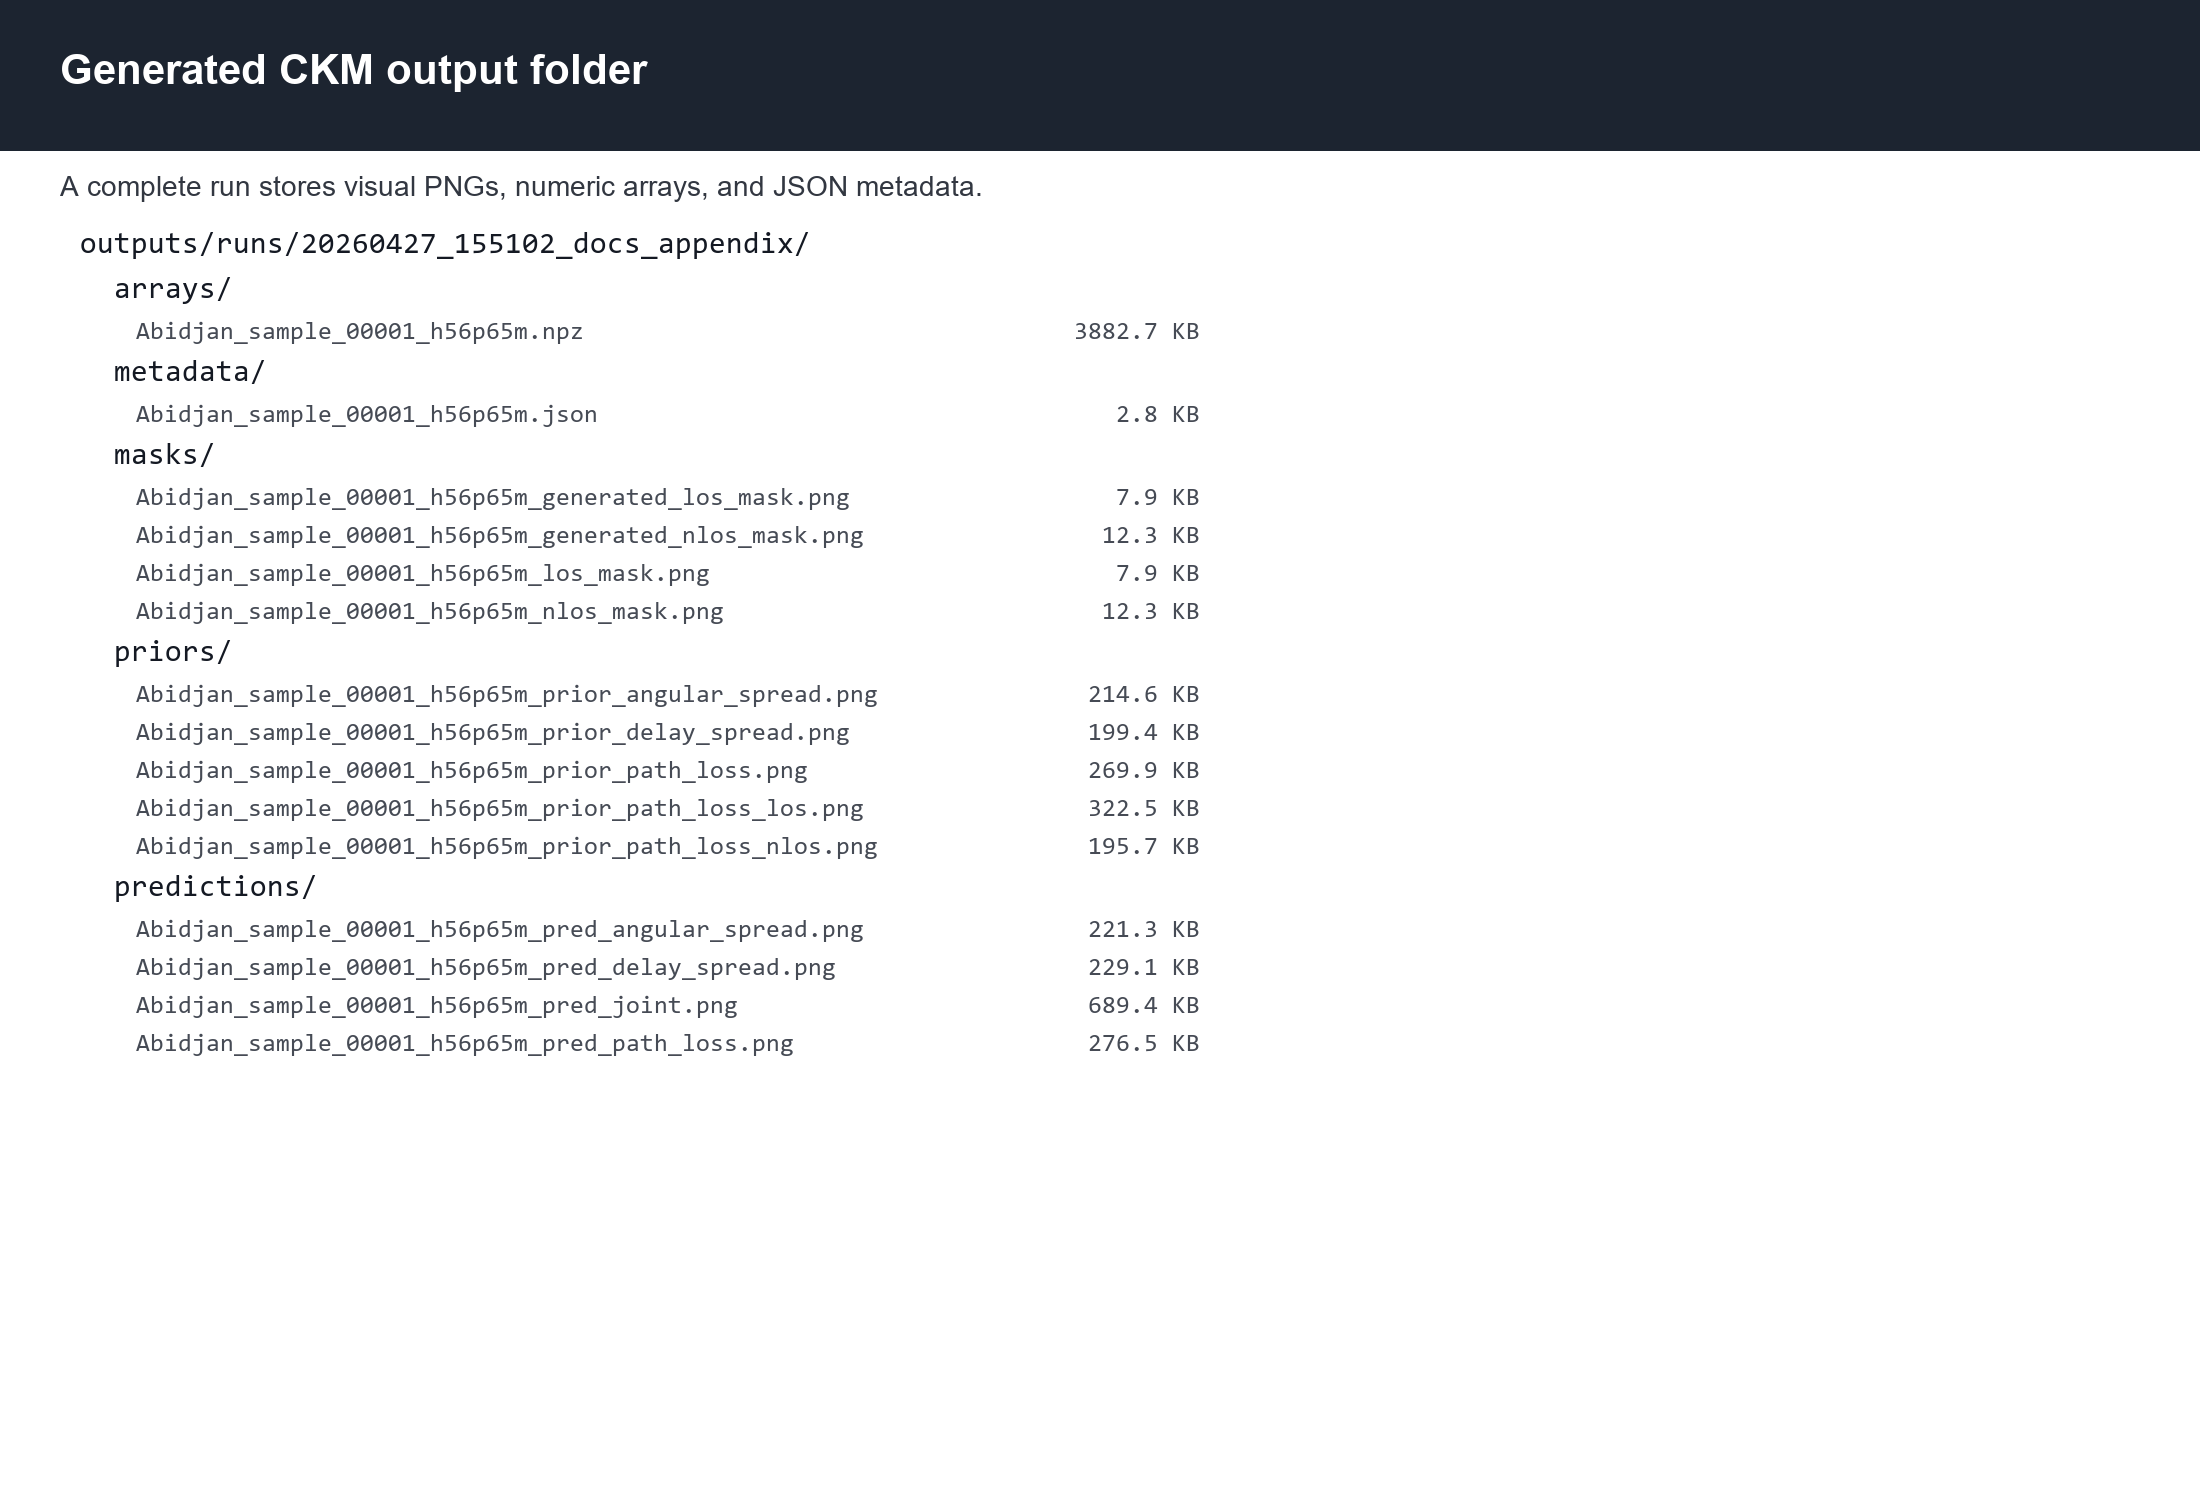
\includegraphics[width=\textwidth,height=0.72\textheight,keepaspectratio]{img/thesis_figures/ckm_generator/ckm_generator_output_tree.png}
\caption[Generated output folder for one run.]%
{Generated output folder for one CKM Generator run. The run contains
binary masks, prior maps, prediction maps, a numerical archive, and a JSON
metadata file; the PNG folders are optional visual exports.}
\label{fig:ckm_generator_output_tree}
\end{figure}

\begin{figure}[H]
\centering
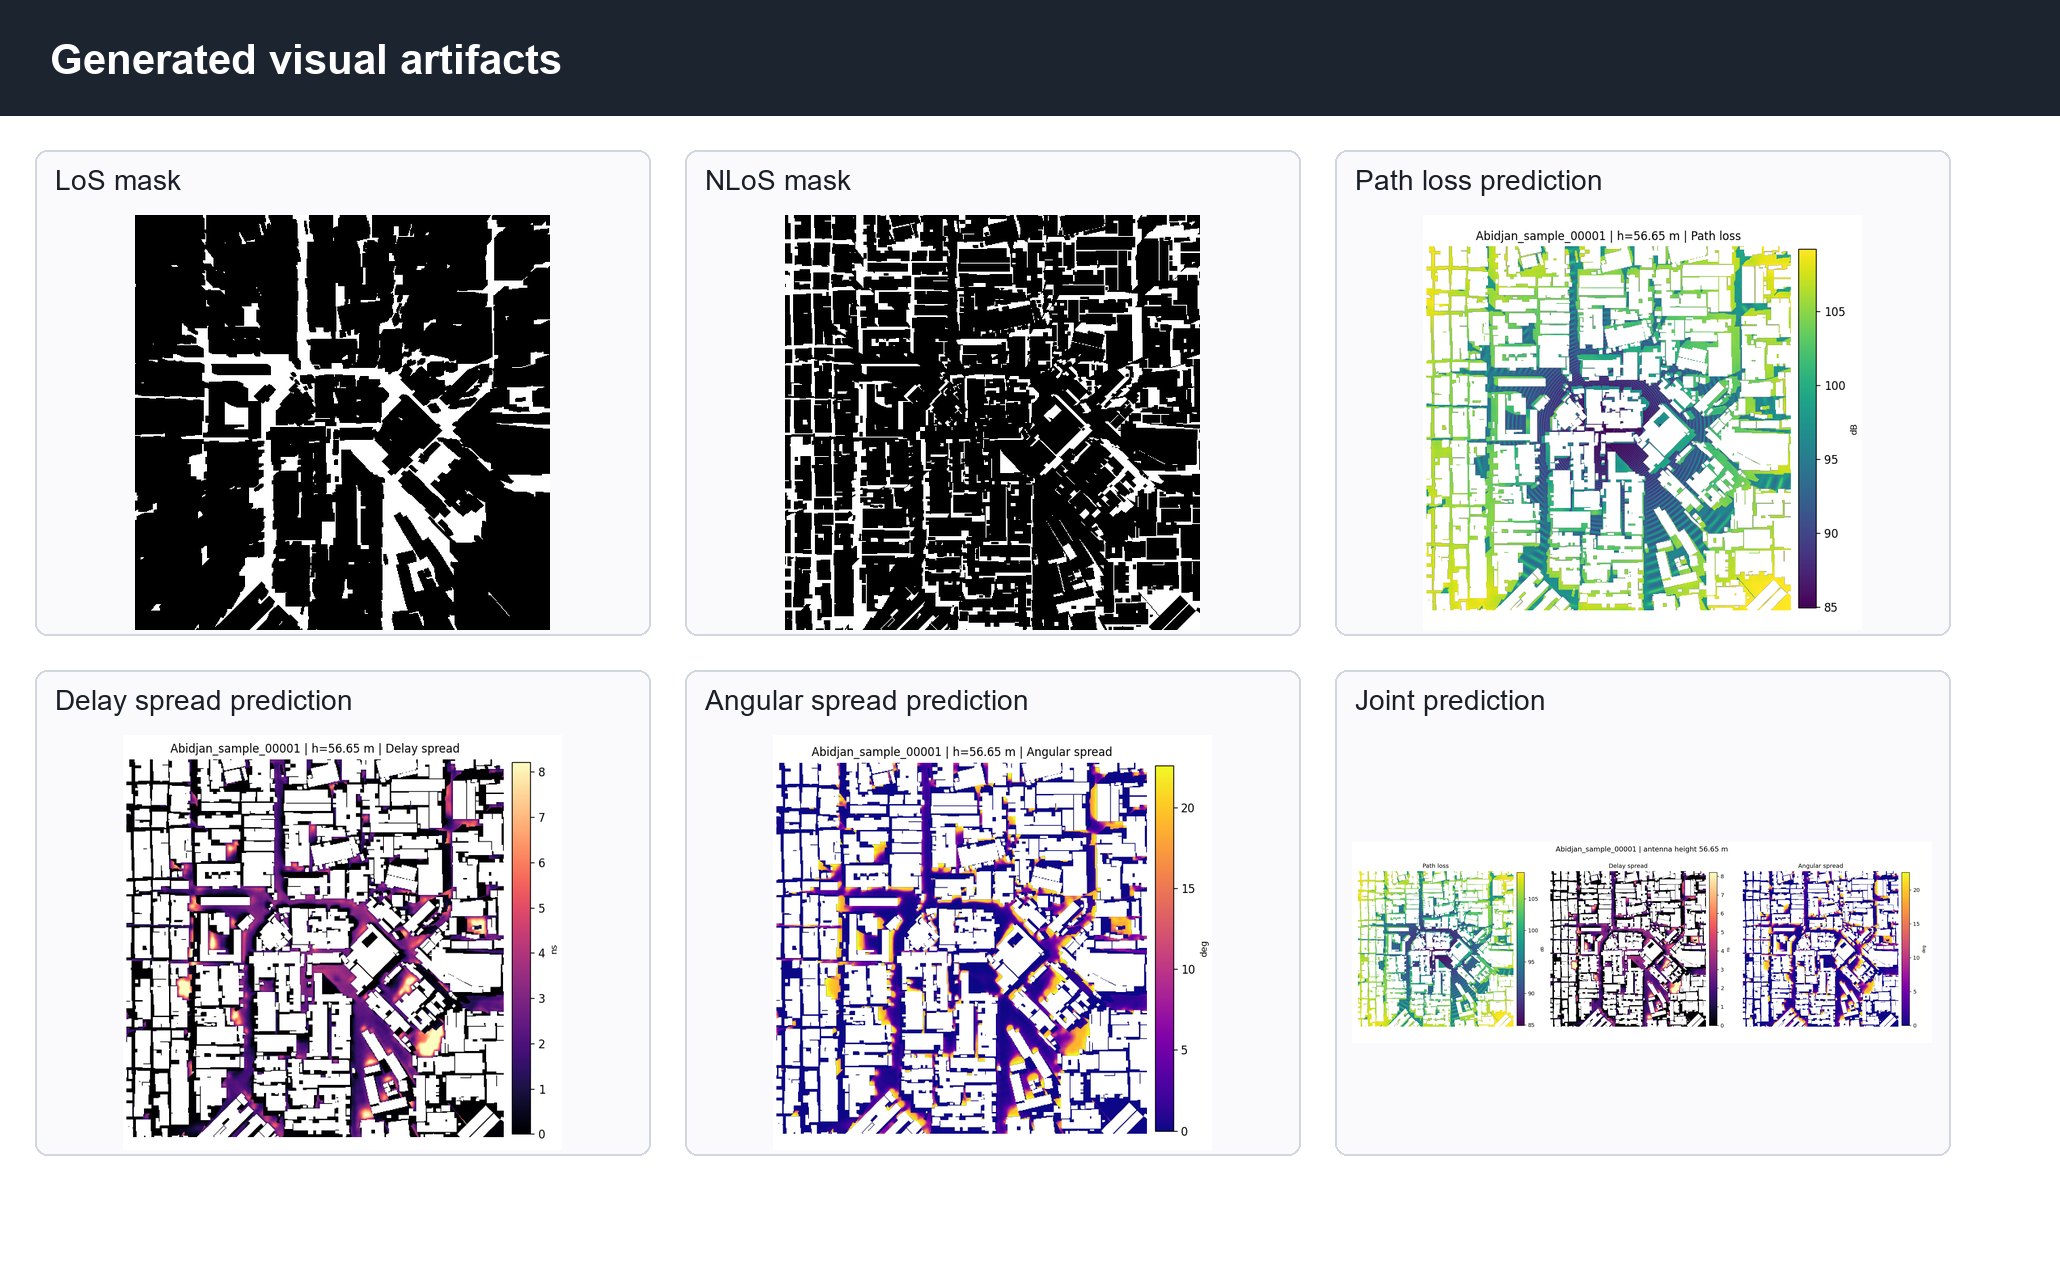
\includegraphics[width=\textwidth,height=0.72\textheight,keepaspectratio]{img/thesis_figures/ckm_generator/ckm_generator_output_visuals.png}
\caption[Visual outputs for one generated sample.]%
{Visual outputs generated for the same sample: LoS/NLoS masks and the
three final-model prediction products, together with the saved joint prediction
panel.}
\label{fig:ckm_generator_output_visuals}
\end{figure}

\begin{figure}[H]
\centering
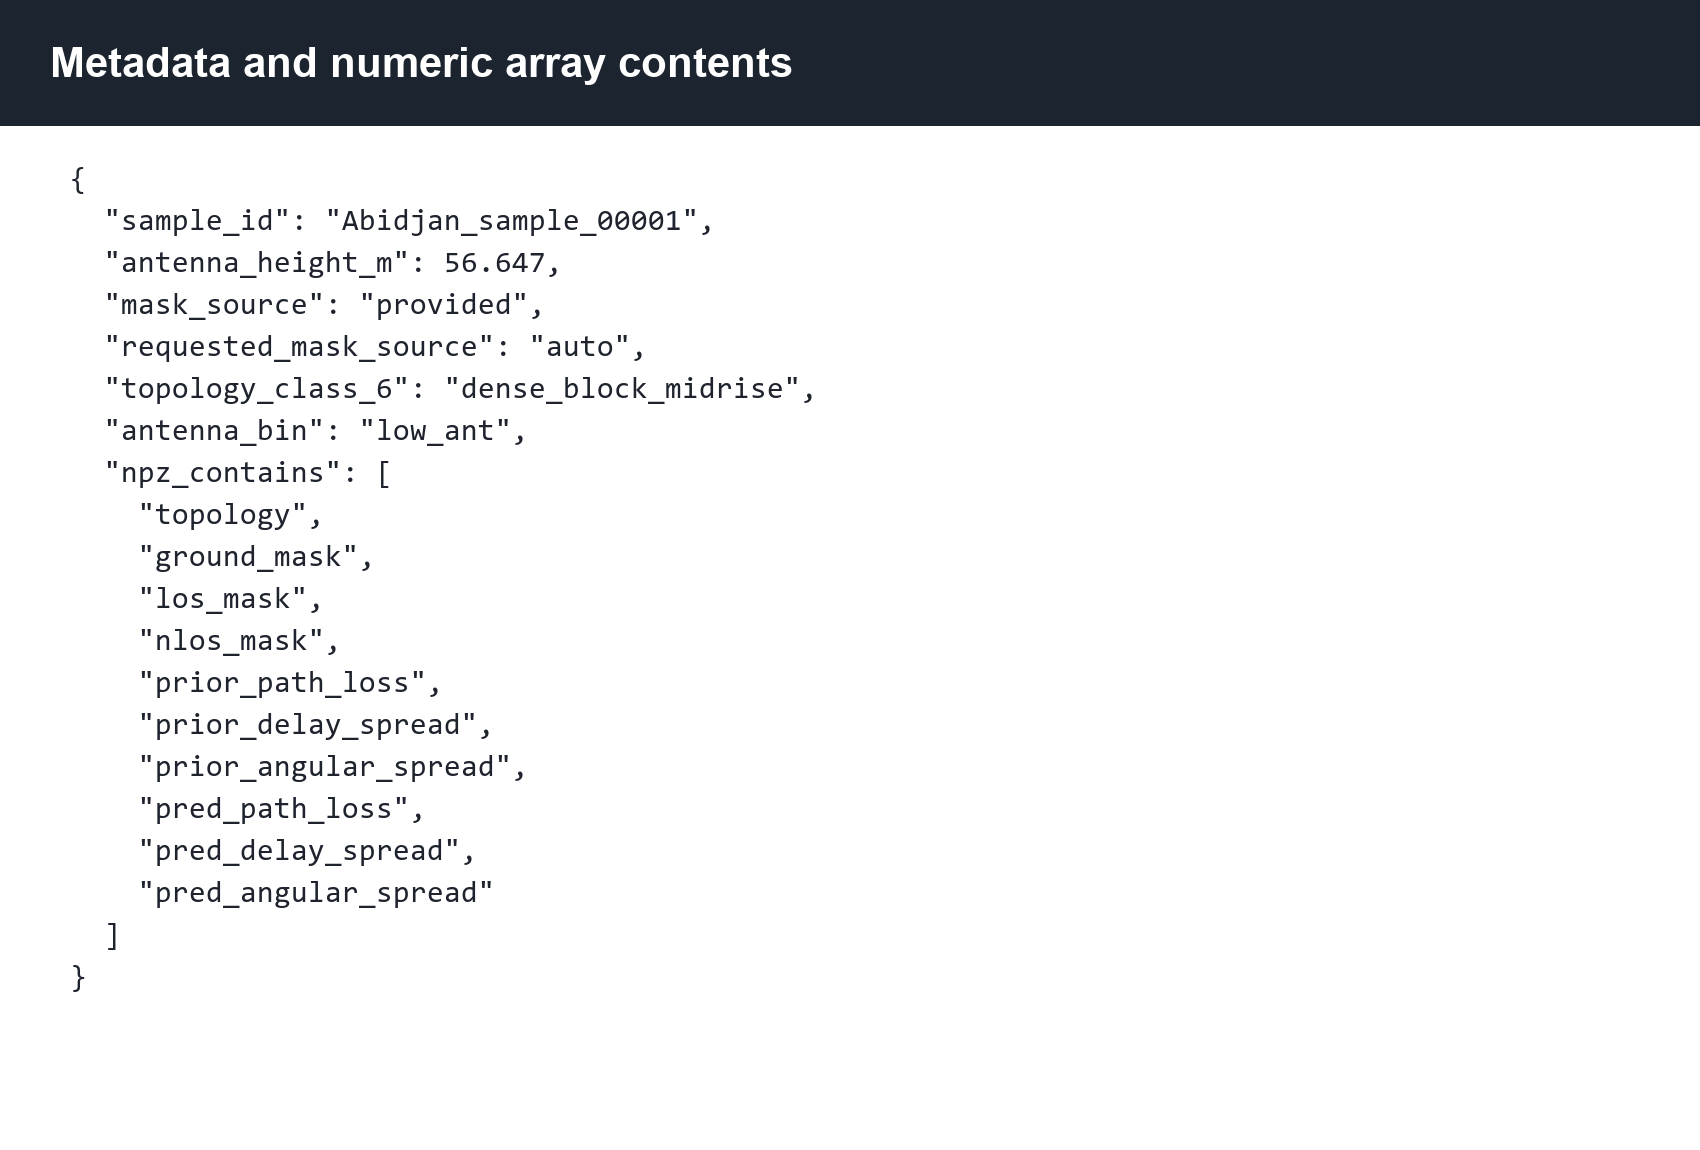
\includegraphics[width=\textwidth,height=0.64\textheight,keepaspectratio]{img/thesis_figures/ckm_generator/ckm_generator_output_metadata.png}
\caption[Generated sample metadata and arrays.]%
{Example metadata and numerical-array contents for a generated sample.
The metadata records provenance and the resolved mask policy, while the
\texttt{.npz} archive keeps the actual \(513\times513\) numeric maps.}
\label{fig:ckm_generator_output_metadata}
\end{figure}

PNG files are visual inspection products. The authoritative numerical output
is the NumPy archive in \texttt{arrays/}. It is uncompressed by default for
faster batch export and compressed only when \texttt{Compress numeric arrays}
or \texttt{--compress-arrays} is enabled. It stores all arrays on the final
\(513\times513\) grid. Important keys include:
\texttt{topology}, \texttt{ground\_mask}, \texttt{los\_mask},
\texttt{nlos\_mask}, \texttt{generated\_los\_mask},
\texttt{generated\_nlos\_mask}, \texttt{reference\_los\_mask} when available,
\texttt{prior\_path\_loss}, \texttt{prior\_path\_loss\_los},
\texttt{prior\_path\_loss\_nlos}, \texttt{prior\_delay\_spread},
\texttt{prior\_angular\_spread}, \texttt{pred\_path\_loss},
\texttt{pred\_delay\_spread}, and \texttt{pred\_angular\_spread}.

The JSON metadata stores provenance and bookkeeping: sample id, antenna height,
source file, checkpoint path, requested and resolved mask source, topology
class, antenna bin, mask comparison statistics when a reference mask exists,
the selected save options, save timings, and the paths of all generated files.

\section{Performance controls}

CUDA is the preferred runtime when available. The app and CLI can also use CPU
or DirectML. The model batch size can increase throughput on GPUs with enough
VRAM, while keeping batch size 1 remains the safest option on smaller cards.

The benchmarked fast path is the same one reported in
Chapter~\ref{chap:results}: vectorized LoS/NLoS mask generation, torch prior
evaluation, mixed-precision neural inference, and default numerical
\texttt{.npz} export after the checkpoint has already been loaded. The appendix
keeps only the operational interpretation: mask generation and prior evaluation
are implementation optimizations, not changes in the mathematical definition of
the generator. The vectorized mask backend was checked against the original
GT ray-caster with zero LoS/NLoS differences on the Barcelona benchmark and on
100 exported CKM samples, while the torch prior backend changed RMSE only in
the fourth decimal place relative to the NumPy prior implementation.

The mixed-precision numerical difference remains negligible. On the full
Barcelona subset, the RMSE between mixed precision and fp32 predictions was
\SI{0.0014}{dB} for path loss, \SI{0.0028}{ns} for delay spread, and
\SI{0.0025}{\degree} for angular spread, which is far below the validation RMSE
scale of the model. Its benefit is speed: with the torch prior backend and
provided masks, the same 50-sample validation path took \SI{0.72}{s} per map in
fp32 and \SI{0.62}{s} per map with CUDA mixed precision.

For batch export, keeping \texttt{Save visual map PNGs},
\texttt{Save LoS/NLoS mask PNGs}, and \texttt{Compress numeric arrays}
disabled avoids Matplotlib rendering and compression overhead while preserving
the masks, priors, predictions, and metadata in the numerical archive.
Disabling \texttt{Run final residual model} is useful when the goal is only to
validate topologies, masks, and prior generation.

\chapter{Additional Results and Qualitative Diagnostics}
\label{app:qualitative_diagnostics}

The most important visual diagnosis was the contrast between plausible LoS
maps and failed NLoS tails. Early CNN outputs often followed the central radial
trend but underestimated shadowed regions. The later histogram analysis made
this visible: the model behaved like a single-mode regressor even when the
target distribution was multi-modal.

This appendix keeps the detailed results that were removed from the main
Results chapter during the reduction pass. They are not needed to follow the
main thesis claim, but they make the final interpretation auditable: the
distribution-first models exposed the target shapes, the final model improved
the frozen priors across splits and regimes, and the runtime optimizations did
not change the mathematical definition of the generator.

\begin{figure}[H]
\centering

\includegraphics[width=\textwidth]{img/thesis_figures/results_addendum/try76_los_vs_nlos_distribution.png}
\caption[Path-loss GMM target fits by topology expert.]%
{Five-component Gaussian-mixture fits of the LoS and NLoS path-loss targets,
shown separately for the six topology experts. This is the distribution seen
by the specialised expert models, and is therefore more faithful than a single
collapsed global curve. Per expert, the target is treated as a GMM rather than
as a perfect Gaussian: the LoS and NLoS marginals contain asymmetric shoulders,
tails and rare outliers, including values outside the visible
\SIrange{72}{128}{dB} plotting window. The solid curves show the total mixture
density and the faint dotted curves show the individual Gaussian components.
The dashed line marks the per-expert marginal mean.}
\label{fig:try76_los_vs_nlos_distribution}
\end{figure}

\begin{figure}[H]
\centering
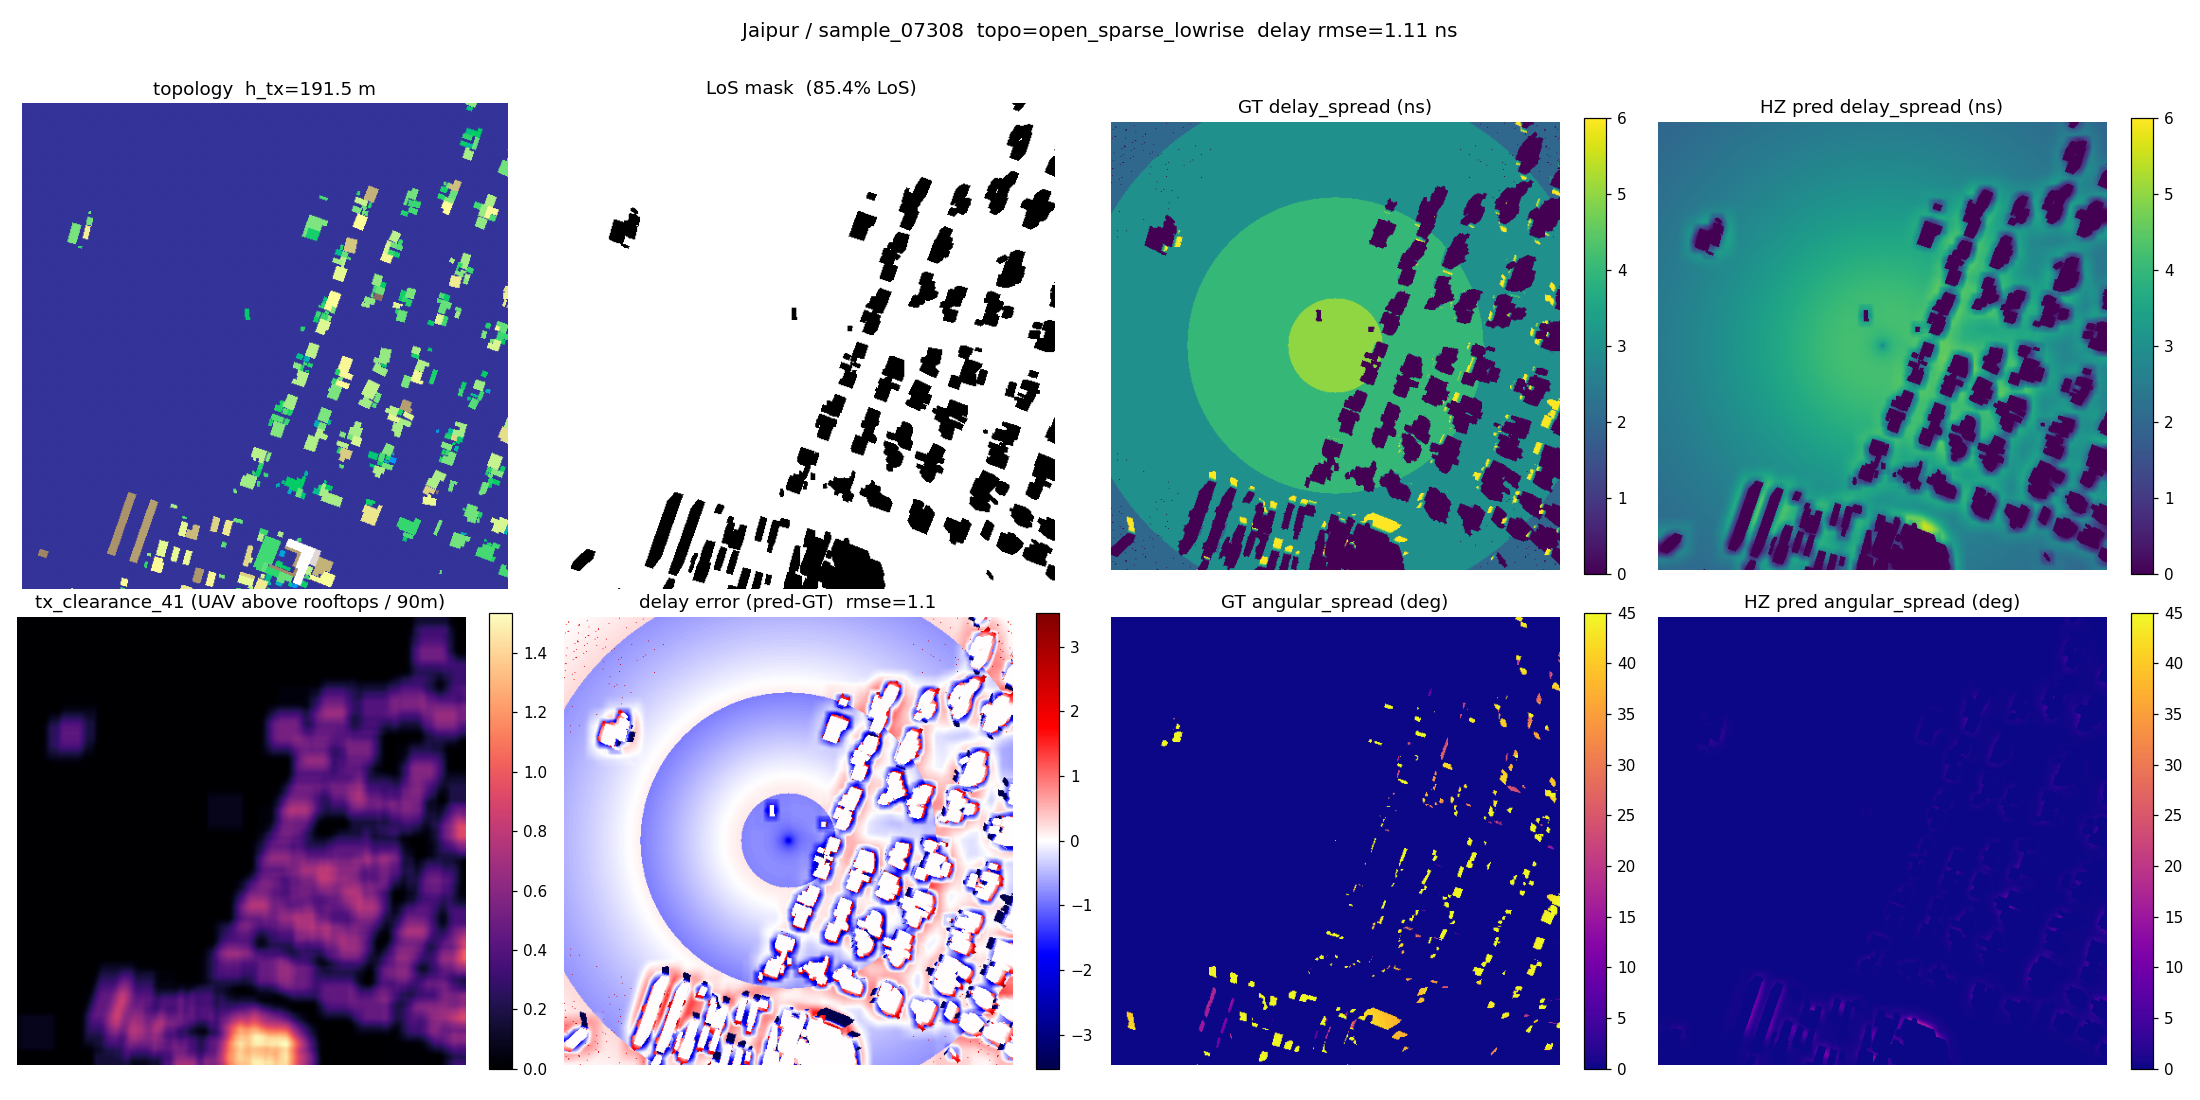
\includegraphics[width=\textwidth]{img/thesis_figures/results_addendum/try79_quantized_spread_example.png}
\caption[Example of spread-target quantisation.]%
{Example of spread-target quantisation on a calibrated-prior test sample
(Jaipur, \texttt{sample\_07308}). The ground-truth delay-spread map contains
broad staircase-like bands and isolated quantised pixels, while the
height-aware calibrated prediction is smoother and more continuous. The
resulting delay RMSE is only \SI{1.11}{ns}, but the residual panel shows how
RMSE still penalises smooth transitions across quantised ground-truth
boundaries. The same effect is visible on the angular-spread map, whose target
is dominated by sparse high-valued quantised pixels.}
\label{fig:try79_quantized_spread_example}
\end{figure}

\begin{figure}[p]
\centering

\includegraphics[width=\textwidth,height=0.82\textheight,keepaspectratio]{img/thesis_figures/distribution_histograms/target_prediction_histograms.png}
\caption[Late path-loss diagnostic histograms.]%
{Late diagnostic path-loss histograms on the validation samples with UAV
heights between \SI{45}{m} and \SI{55}{m}. This stage exposed the NLoS
path-loss mode collapse that motivated the distribution-first and
prior-anchored final attempts. The binned curves are lightly smoothed for
readability.}
\label{fig:try74_75_diagnostic_histograms_results}
\end{figure}

\begin{figure}[p]
\centering
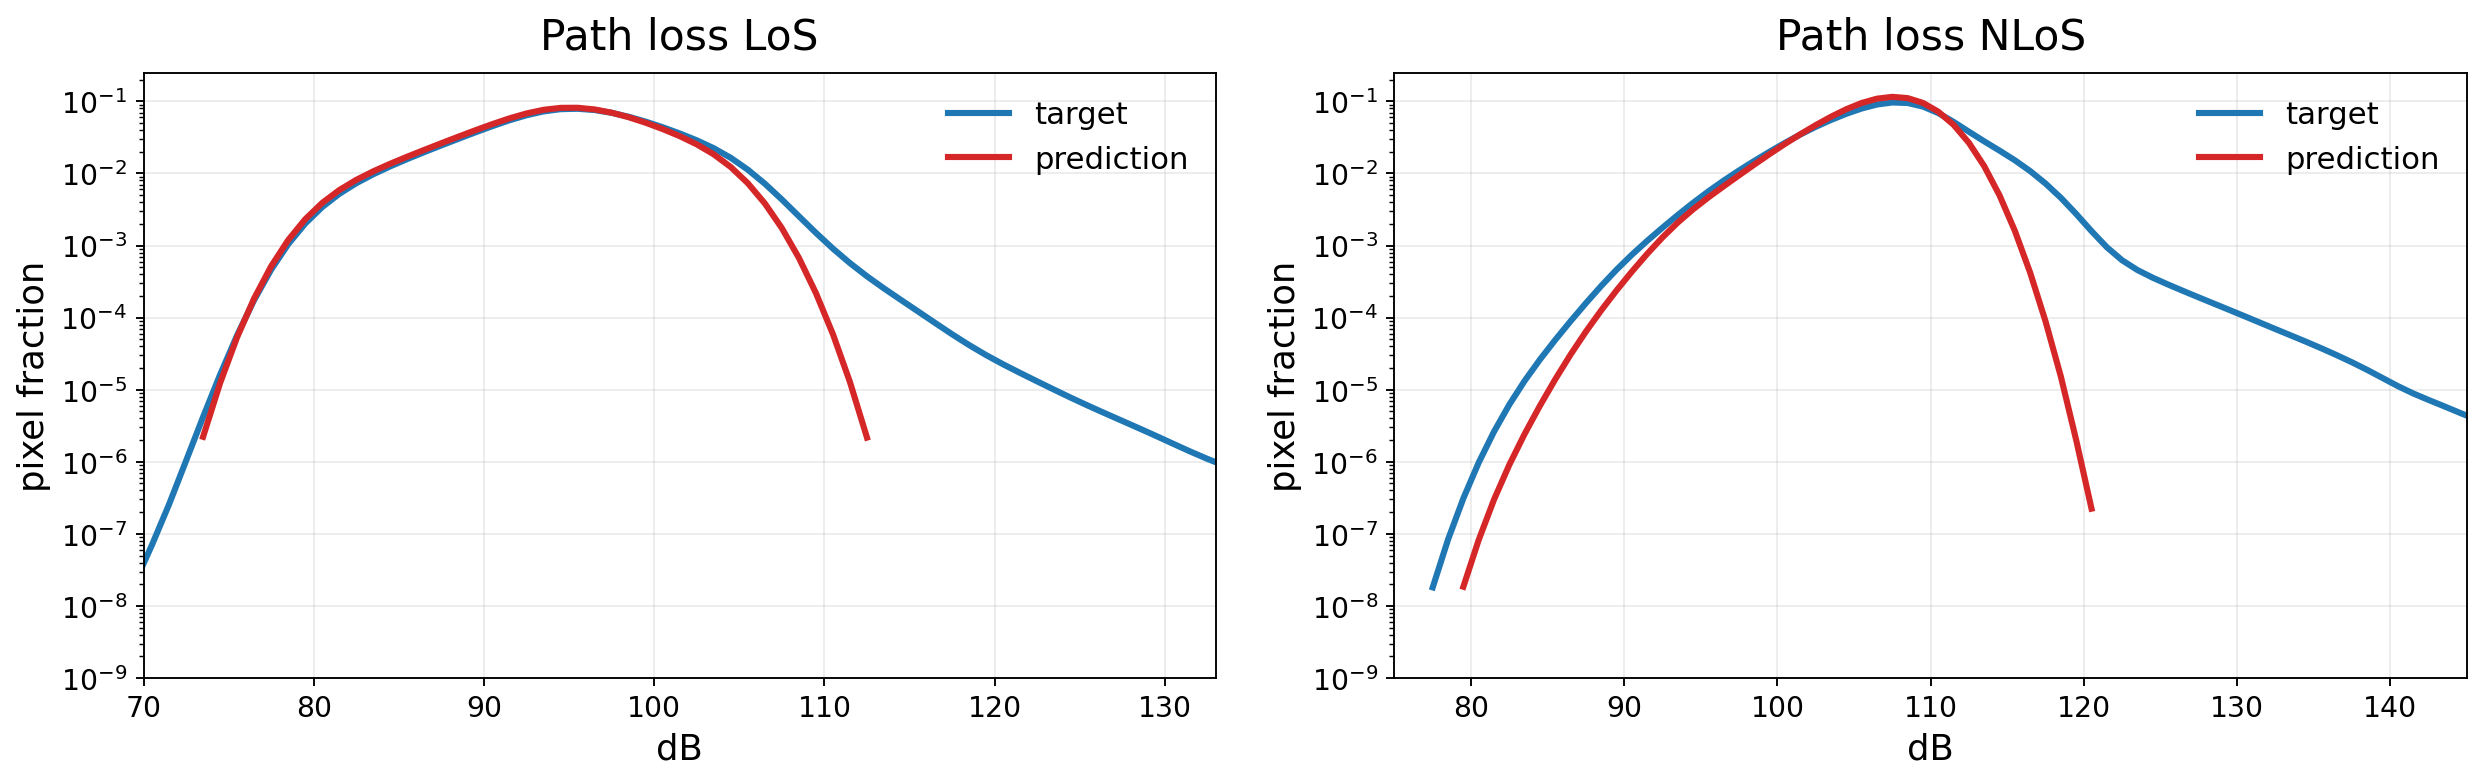
\includegraphics[width=\textwidth,height=0.82\textheight,keepaspectratio]{img/thesis_figures/results_addendum/try80_validation_45_55_target_prediction_histograms.png}
\caption[Final validation histograms on the same 45--55 m subset.]%
{Final prior-anchored residual GMM-head path-loss histograms on the same
validation subset and with the same plotting convention as
Figure~\ref{fig:try74_75_diagnostic_histograms_results}. The path-loss panels
show that the final model removes the severe NLoS mode collapse.}
\label{fig:try80_validation_45_55_histograms}
\end{figure}

\begin{figure}[H]
\centering
\pgfplotsset{
  stagebar/.style={
    ybar, width=4.2cm, height=5.3cm, ymin=0,
    enlarge x limits=0.55,
    bar width=14pt,
    nodes near coords,
    nodes near coords style={font=\scriptsize},
    xticklabel style={rotate=35,anchor=east,font=\scriptsize},
    title style={font=\small},
    grid=major,
  }
}
\begin{minipage}{0.31\textwidth}\centering
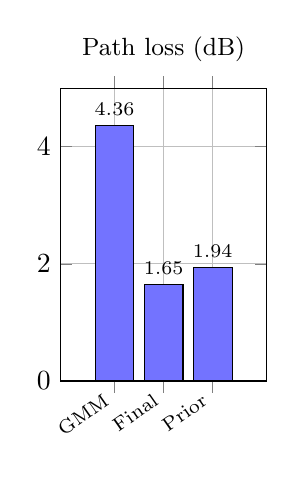
\begin{tikzpicture}
\begin{axis}[
  stagebar,
  title={Path loss (dB)},
  ymax=5.0,
  symbolic x coords={GMM,Final,Prior},
  xtick=data,
  xticklabels={GMM,Final,Prior},
]
\addplot[fill=blue!55] coordinates {(GMM,4.36) (Final,1.65) (Prior,1.94)};
\end{axis}
\end{tikzpicture}
\end{minipage}
\hfill
\begin{minipage}{0.31\textwidth}\centering
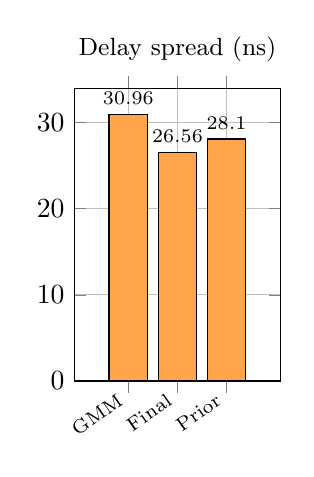
\begin{tikzpicture}
\begin{axis}[
  stagebar,
  title={Delay spread (ns)},
  ymax=34,
  symbolic x coords={GMM,Final,Prior},
  xtick=data,
  xticklabels={GMM,Final,Prior},
]
\addplot[fill=orange!70] coordinates {(GMM,30.96) (Final,26.56) (Prior,28.10)};
\end{axis}
\end{tikzpicture}
\end{minipage}
\hfill
\begin{minipage}{0.31\textwidth}\centering
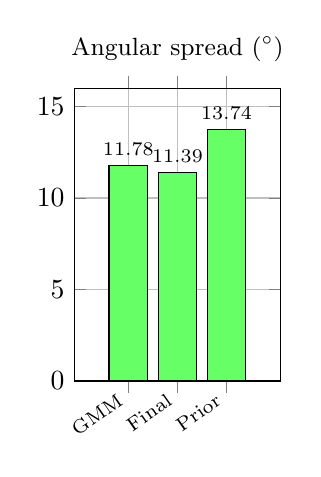
\begin{tikzpicture}
\begin{axis}[
  stagebar,
  title={Angular spread ($^\circ$)},
  ymax=16,
  symbolic x coords={GMM,Final,Prior},
  xtick=data,
  xticklabels={GMM,Final,Prior},
]
\addplot[fill=green!60] coordinates {(GMM,11.78) (Final,11.39) (Prior,13.74)};
\end{axis}
\end{tikzpicture}
\end{minipage}
\caption[Final model compared with prior and GMM references.]%
{Test-set comparison between the distribution-first neural references
and the final prior-anchored residual GMM-head model. The path-loss panel uses global
pixel-weighted RMSE; the spread GMM reference is shown for the two spread targets.}
\label{fig:try76_77_80_prior_comparison}
\end{figure}

\begin{figure}[H]
\centering
{\scriptsize Coloured bars are the final model and grey bars are the frozen prior.\par}
\vspace{0.2em}
\pgfplotsset{
  splitbar/.style={
    ybar, width=4.2cm, height=5.3cm, ymin=0,
    bar width=5pt,
    enlarge x limits=0.18,
    symbolic x coords={Train,Val,Test,All},
    xtick=data,
    xticklabel style={rotate=35,anchor=east,font=\scriptsize},
    title style={font=\small},
    grid=major,
  }
}
\begin{minipage}{0.31\textwidth}\centering
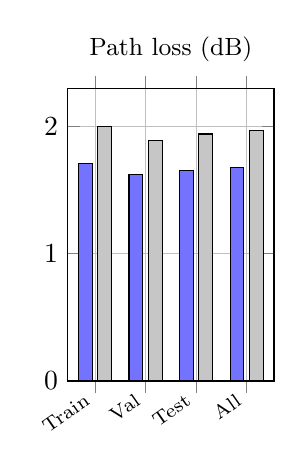
\begin{tikzpicture}
\begin{axis}[splitbar, title={Path loss (dB)}, ymax=2.3]
\addplot[fill=blue!55] coordinates {(Train,1.71) (Val,1.62) (Test,1.65) (All,1.68)};
\addplot[fill=gray!45] coordinates {(Train,2.00) (Val,1.89) (Test,1.94) (All,1.97)};
\end{axis}
\end{tikzpicture}
\end{minipage}
\hfill
\begin{minipage}{0.31\textwidth}\centering
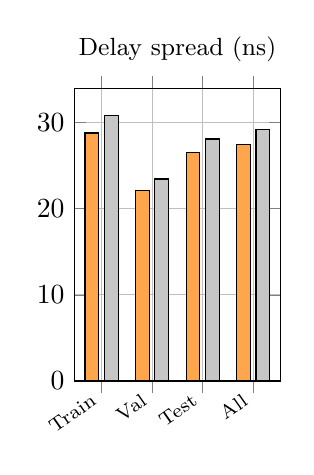
\begin{tikzpicture}
\begin{axis}[splitbar, title={Delay spread (ns)}, ymax=34]
\addplot[fill=orange!70] coordinates {(Train,28.79) (Val,22.11) (Test,26.56) (All,27.41)};
\addplot[fill=gray!45] coordinates {(Train,30.81) (Val,23.45) (Test,28.10) (All,29.25)};
\end{axis}
\end{tikzpicture}
\end{minipage}
\hfill
\begin{minipage}{0.31\textwidth}\centering
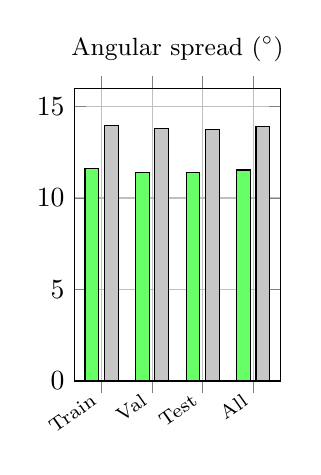
\begin{tikzpicture}
\begin{axis}[splitbar, title={Angular spread ($^\circ$)}, ymax=16]
\addplot[fill=green!60] coordinates {(Train,11.60) (Val,11.38) (Test,11.39) (All,11.53)};
\addplot[fill=gray!45] coordinates {(Train,13.96) (Val,13.82) (Test,13.74) (All,13.90)};
\end{axis}
\end{tikzpicture}
\end{minipage}
\caption[Final model versus frozen priors by split.]%
{Final model versus the frozen prior across train, validation, unseen test,
and all-city aggregation. Validation is the model-selection split; test
contains cities not seen during training.}
\label{fig:try80_split_rmse}
\end{figure}

\begin{table}[H]
\centering
\caption[Final-model RMSE by split.]%
{Final-model pixel-weighted RMSE by split, compared with the frozen priors.
The test split is the unseen-city generalisation claim; the all row aggregates
train, validation, and test together.}
\label{tab:try80_split_absolute}
\scriptsize
\begin{tabular}{lrrrrrrr}
\toprule
Split & Samples & PL model & PL prior & DS model & DS prior & AS model & AS prior \\
\midrule
Train & 10840 & 1.7111 & 2.0006 & 28.7929 & 30.8086 & 11.5975 & 13.9553 \\
Validation & 2750 & 1.6157 & 1.8916 & 22.1061 & 23.4494 & 11.3782 & 13.8178 \\
Test & 2590 & 1.6519 & 1.9383 & 26.5570 & 28.1023 & 11.3854 & 13.7416 \\
All & 16180 & 1.6845 & 1.9711 & 27.4121 & 29.2527 & 11.5256 & 13.8966 \\
\bottomrule
\end{tabular}
\end{table}

\begin{table}[H]
\centering
\caption[Final-model improvement by split.]%
{Final-model improvement over the frozen priors by split. Values are
pixel-weighted \(\Delta=\mathrm{model}-\mathrm{prior}\); negative values are
better.}
\label{tab:try80_split_delta}
\scriptsize
\begin{tabular}{lrrrrrrr}
\toprule
Split & Samples & PL \(\Delta\)RMSE & PL \(\Delta\)MAE & DS \(\Delta\)RMSE & DS \(\Delta\)MAE & AS \(\Delta\)RMSE & AS \(\Delta\)MAE \\
\midrule
Train & 10840 & -0.2895 & -0.3030 & -2.0157 & +0.6135 & -2.3578 & +0.0108 \\
Validation & 2750 & -0.2758 & -0.2865 & -1.3433 & +0.5869 & -2.4396 & -0.0413 \\
Test & 2590 & -0.2865 & -0.3020 & -1.5453 & +0.6864 & -2.3562 & +0.0198 \\
All & 16180 & -0.2867 & -0.3000 & -1.8406 & +0.6214 & -2.3710 & +0.0036 \\
\bottomrule
\end{tabular}
\end{table}

\begin{figure}[ht]
\centering
\pgfplotsset{
  barplot/.style={
    ybar, width=4.2cm, height=5.5cm, ymin=0,
    enlarge x limits=0.6,
    symbolic x coords={model,prior},
    xtick=data,
    xticklabels={Final, Prior},
    nodes near coords,
    nodes near coords style={font=\footnotesize},
    nodes near coords align={vertical},
    grid=major,
  }
}
\begin{minipage}{0.31\textwidth}\centering
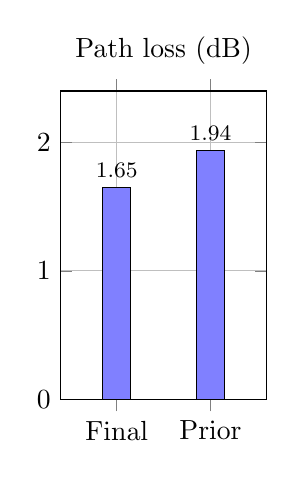
\begin{tikzpicture}
\begin{axis}[barplot, title={Path loss (dB)}, ymax=2.4]
\addplot[fill=blue!50] coordinates {(model,1.65) (prior,1.94)};
\end{axis}
\end{tikzpicture}
\end{minipage}
\hfill
\begin{minipage}{0.31\textwidth}\centering
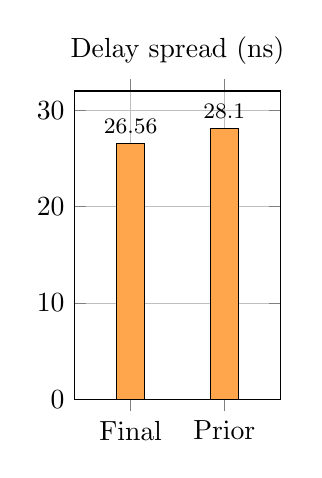
\begin{tikzpicture}
\begin{axis}[barplot, title={Delay spread (ns)}, ymax=32]
\addplot[fill=orange!70] coordinates {(model,26.56) (prior,28.10)};
\end{axis}
\end{tikzpicture}
\end{minipage}
\hfill
\begin{minipage}{0.31\textwidth}\centering
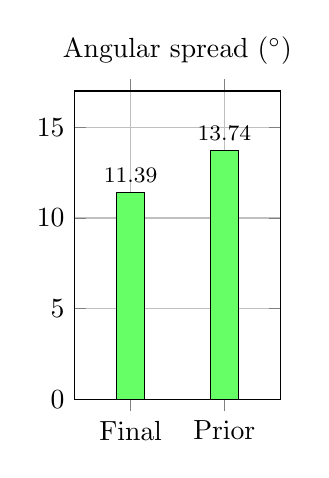
\begin{tikzpicture}
\begin{axis}[barplot, title={Angular spread ($^\circ$)}, ymax=17]
\addplot[fill=green!60] coordinates {(model,11.39) (prior,13.74)};
\end{axis}
\end{tikzpicture}
\end{minipage}
\caption[Final test RMSE against frozen priors.]%
{Final test RMSE on unseen cities against the frozen priors for
path loss, delay spread, and angular spread.}
\label{fig:try80_test_final}
\end{figure}

\begin{figure}[H]
\centering
\pgfplotsset{
  targetcompare/.style={
    ybar, width=\linewidth, height=5.4cm, ymin=0,
    bar width=18pt,
    symbolic x coords={Target,Final},
    xtick={Target,Final},
    xticklabel style={font=\small},
    tick label style={font=\small},
    title style={font=\bfseries\small},
    enlarge x limits=0.35,
    ymajorgrids=true,
    nodes near coords,
    every node near coord/.append style={font=\scriptsize},
  }
}
\begin{minipage}{0.31\textwidth}\centering
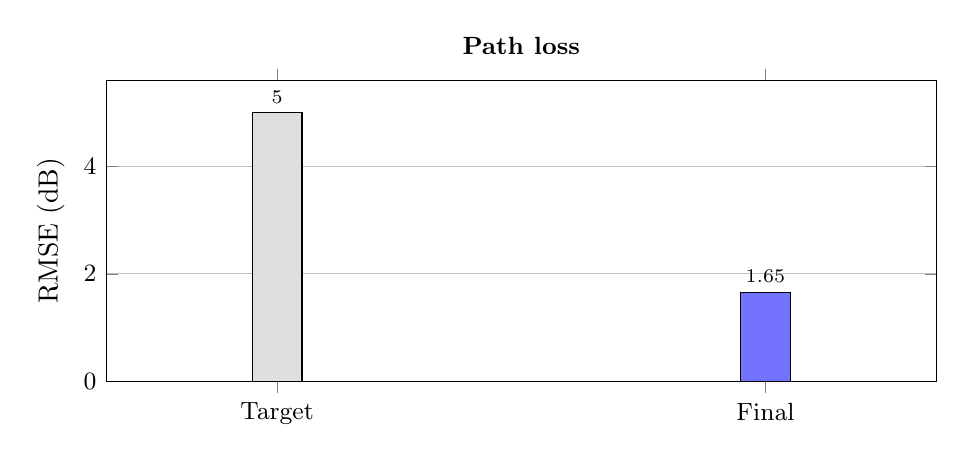
\begin{tikzpicture}
\begin{axis}[targetcompare, title={Path loss}, ylabel={RMSE (dB)}, ymax=5.6]
\addplot[fill=gray!25, draw=black, bar shift=0pt] coordinates {(Target,5.00)};
\addplot[fill=blue!55, draw=black, bar shift=0pt] coordinates {(Final,1.65)};
\end{axis}
\end{tikzpicture}
\end{minipage}
\hfill
\begin{minipage}{0.31\textwidth}\centering
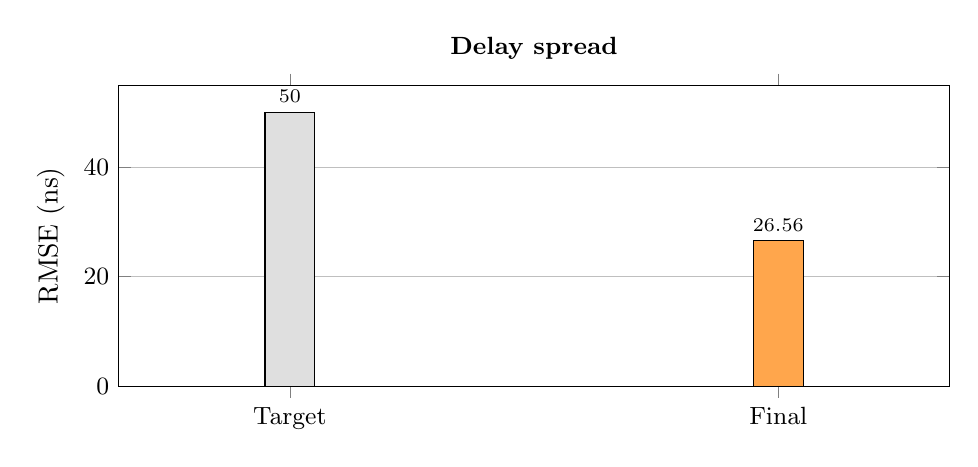
\begin{tikzpicture}
\begin{axis}[targetcompare, title={Delay spread}, ylabel={RMSE (ns)}, ymax=55]
\addplot[fill=gray!25, draw=black, bar shift=0pt] coordinates {(Target,50.00)};
\addplot[fill=orange!70, draw=black, bar shift=0pt] coordinates {(Final,26.56)};
\end{axis}
\end{tikzpicture}
\end{minipage}
\hfill
\begin{minipage}{0.31\textwidth}\centering
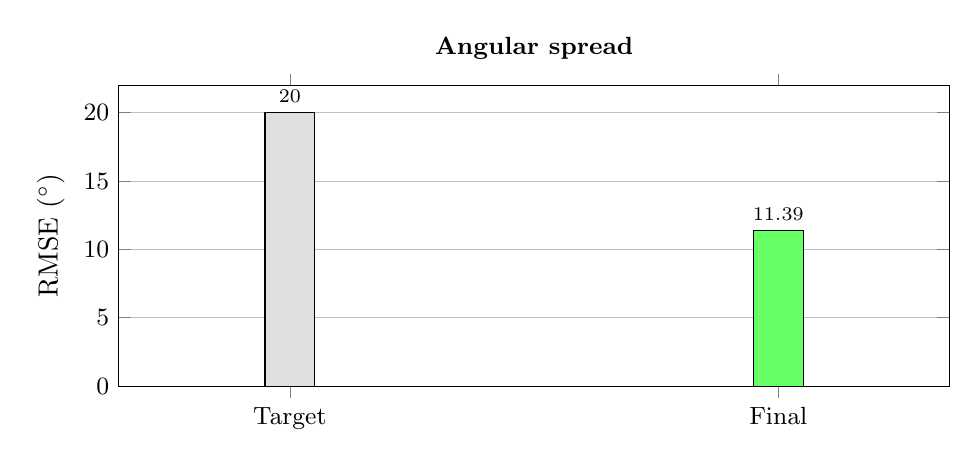
\begin{tikzpicture}
\begin{axis}[targetcompare, title={Angular spread}, ylabel={RMSE ($^\circ$)}, ymax=22]
\addplot[fill=gray!25, draw=black, bar shift=0pt] coordinates {(Target,20.00)};
\addplot[fill=green!60, draw=black, bar shift=0pt] coordinates {(Final,11.39)};
\end{axis}
\end{tikzpicture}
\end{minipage}
\caption[Final result against original numerical targets.]%
{\textbf{Target vs final result.} Final global test check using
pixel-weighted RMSE only. The final-result bar is the held-out city test
result, which remains below the original targets: \SI{5}{dB} for path loss,
\SI{50}{ns} for delay spread, and \(20^\circ\) for angular spread.}
\label{fig:try80_test_objectives}
\end{figure}

\begin{figure}[H]
\centering
{\scriptsize Coloured bars are the final model and grey bars are the frozen prior.\par}
\vspace{0.2em}
\pgfplotsset{
  regimebar/.style={
    ybar, width=4.2cm, height=5.2cm, ymin=0,
    bar width=9pt,
    enlarge x limits=0.45,
    symbolic x coords={LoS,NLoS},
    xtick=data,
    title style={font=\small},
    grid=major,
  }
}
\begin{minipage}{0.31\textwidth}\centering
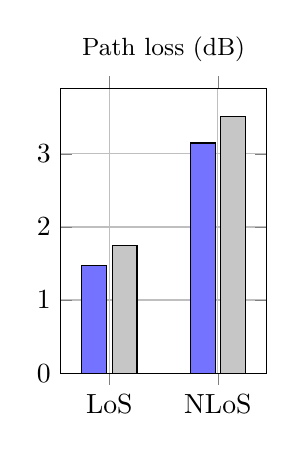
\begin{tikzpicture}
\begin{axis}[regimebar, title={Path loss (dB)}, ymax=3.9]
\addplot[fill=blue!55] coordinates {(LoS,1.47) (NLoS,3.15)};
\addplot[fill=gray!45] coordinates {(LoS,1.75) (NLoS,3.51)};
\end{axis}
\end{tikzpicture}
\end{minipage}
\hfill
\begin{minipage}{0.31\textwidth}\centering
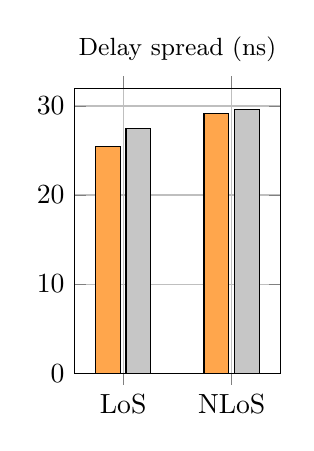
\begin{tikzpicture}
\begin{axis}[regimebar, title={Delay spread (ns)}, ymax=32]
\addplot[fill=orange!70] coordinates {(LoS,25.44) (NLoS,29.20)};
\addplot[fill=gray!45] coordinates {(LoS,27.49) (NLoS,29.62)};
\end{axis}
\end{tikzpicture}
\end{minipage}
\hfill
\begin{minipage}{0.31\textwidth}\centering
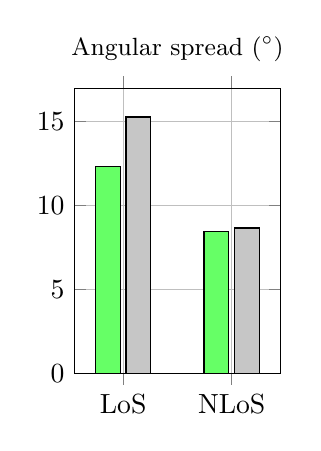
\begin{tikzpicture}
\begin{axis}[regimebar, title={Angular spread ($^\circ$)}, ymax=17]
\addplot[fill=green!60] coordinates {(LoS,12.35) (NLoS,8.44)};
\addplot[fill=gray!45] coordinates {(LoS,15.28) (NLoS,8.66)};
\end{axis}
\end{tikzpicture}
\end{minipage}
\caption[Final test RMSE by LoS and NLoS regime.]%
{Final test RMSE separated by LoS and NLoS pixels. The model
improves the frozen prior in both regimes for all three outputs.}
\label{fig:try80_test_los_nlos}
\end{figure}

\begin{table}[H]
\centering
\caption[Final-model LoS/NLoS improvement by split.]%
{Final-model LoS/NLoS RMSE improvement by split. Values are
pixel-weighted \(\Delta=\mathrm{model}-\mathrm{prior}\); negative values are
better.}
\label{tab:try80_los_nlos_split_delta}
\scriptsize
\begin{tabular}{llrrr}
\toprule
Split & Scope & PL \(\Delta\)RMSE & DS \(\Delta\)RMSE & AS \(\Delta\)RMSE \\
\midrule
Train & LoS & -0.2880 & -2.7919 & -3.0669 \\
Train & NLoS & -0.3640 & -0.4813 & -0.2537 \\
Validation & LoS & -0.2781 & -1.7935 & -3.0430 \\
Validation & NLoS & -0.3103 & -0.3452 & -0.1880 \\
Test & LoS & -0.2844 & -2.0432 & -2.9308 \\
Test & NLoS & -0.3661 & -0.4112 & -0.2191 \\
All & LoS & -0.2856 & -2.5127 & -3.0385 \\
All & NLoS & -0.3565 & -0.4525 & -0.2388 \\
\bottomrule
\end{tabular}
\end{table}

\begin{figure}[H]
\centering
\pgfplotsset{
  subexpertdelta/.style={
    ybar, width=\linewidth, height=5.1cm,
    bar width=5pt,
    symbolic x coords={DH,DM,DL,MH,MM,ML,OH,OM,OL},
    xtick=data,
    xticklabel style={rotate=55,anchor=east,font=\tiny},
    tick label style={font=\tiny},
    title style={font=\small},
    enlarge x limits=0.08,
    ymajorgrids=true,
    ylabel={$\Delta$RMSE},
  }
}
\begin{minipage}{0.31\textwidth}\centering
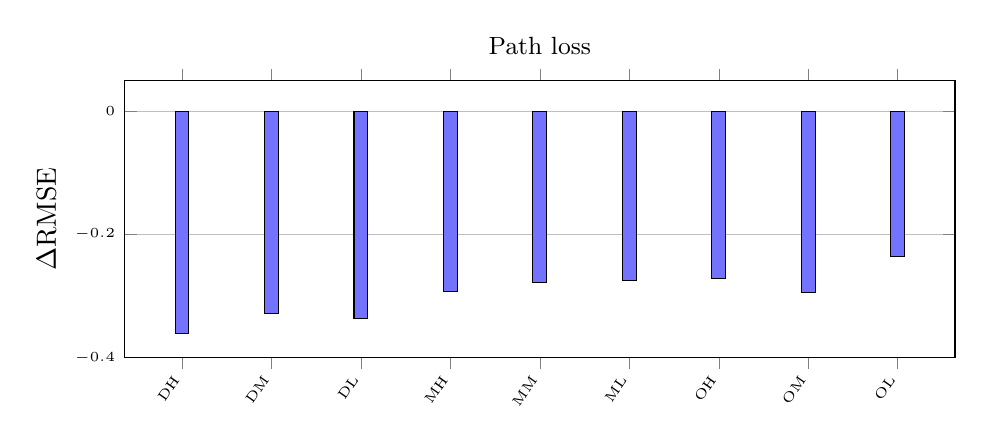
\begin{tikzpicture}
\begin{axis}[subexpertdelta, title={Path loss}, ymin=-0.40, ymax=0.05]
\addplot[fill=blue!55] coordinates {
  (DH,-0.3602) (DM,-0.3288) (DL,-0.3359)
  (MH,-0.2931) (MM,-0.2781) (ML,-0.2745)
  (OH,-0.2721) (OM,-0.2941) (OL,-0.2363)
};
\end{axis}
\end{tikzpicture}
\end{minipage}
\hfill
\begin{minipage}{0.31\textwidth}\centering
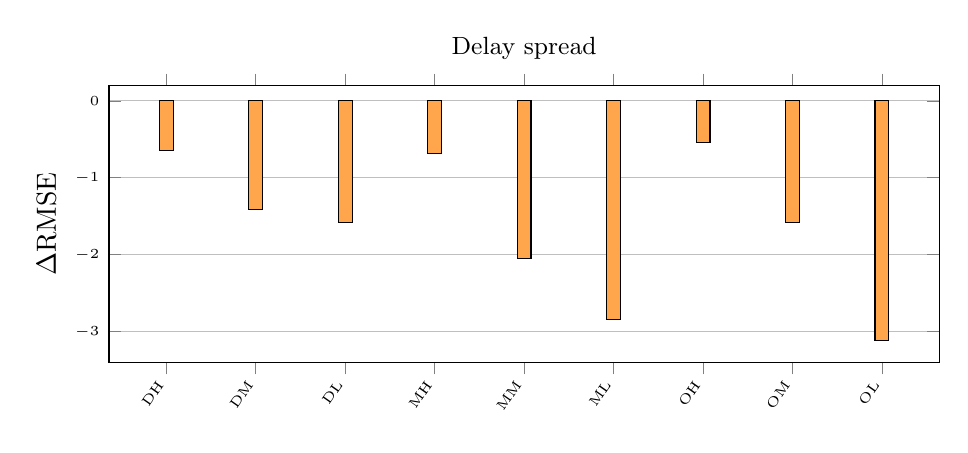
\begin{tikzpicture}
\begin{axis}[subexpertdelta, title={Delay spread}, ymin=-3.4, ymax=0.2]
\addplot[fill=orange!70] coordinates {
  (DH,-0.6473) (DM,-1.4074) (DL,-1.5779)
  (MH,-0.6794) (MM,-2.0522) (ML,-2.8379)
  (OH,-0.5428) (OM,-1.5789) (OL,-3.1170)
};
\end{axis}
\end{tikzpicture}
\end{minipage}
\hfill
\begin{minipage}{0.31\textwidth}\centering
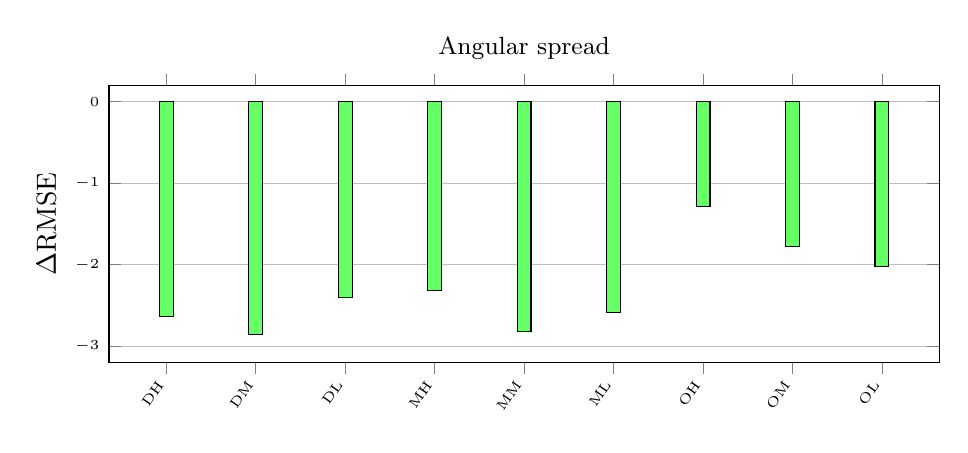
\begin{tikzpicture}
\begin{axis}[subexpertdelta, title={Angular spread}, ymin=-3.2, ymax=0.2]
\addplot[fill=green!60] coordinates {
  (DH,-2.6405) (DM,-2.8587) (DL,-2.3994)
  (MH,-2.3186) (MM,-2.8200) (ML,-2.5845)
  (OH,-1.2874) (OM,-1.7804) (OL,-2.0271)
};
\end{axis}
\end{tikzpicture}
\end{minipage}
\caption[All-city RMSE deltas by prior subexpert.]%
{All-city RMSE deltas by prior subexpert. Negative values mean
that the final model improves the frozen prior. The first letter denotes the morphology
expert (dense, mixed, open) and the second letter the antenna-height expert
(high, low, mid).}
\label{fig:try80_subexpert_delta}
\end{figure}

\begin{table}[H]
\centering
\caption[All-city final-model deltas by prior subexpert.]%
{All-city final-model deltas by prior subexpert. Each city contributes to one
of the nine morphology and antenna prior experts, and the table shows that the
improvement is not concentrated in a single easy subexpert.}
\label{tab:try80_subexpert_delta}
\scriptsize
\begin{tabular}{lrrrrrrr}
\toprule
Subexpert & Samples & PL \(\Delta\)RMSE & PL \(\Delta\)MAE & DS \(\Delta\)RMSE & DS \(\Delta\)MAE & AS \(\Delta\)RMSE & AS \(\Delta\)MAE \\
\midrule
\texttt{dense|high\_ant} & 1957 & -0.3602 & -0.3674 & -0.6473 & +0.0638 & -2.6405 & -0.0905 \\
\texttt{dense|low\_ant} & 2018 & -0.3359 & -0.3303 & -1.5779 & +0.5463 & -2.3994 & -0.1867 \\
\texttt{dense|mid\_ant} & 2055 & -0.3288 & -0.3223 & -1.4074 & +0.6147 & -2.8587 & -0.2663 \\
\texttt{mixed|high\_ant} & 2156 & -0.2931 & -0.3308 & -0.6794 & +0.2382 & -2.3186 & +0.0025 \\
\texttt{mixed|low\_ant} & 2060 & -0.2745 & -0.2514 & -2.8379 & +0.8299 & -2.5845 & -0.0666 \\
\texttt{mixed|mid\_ant} & 2094 & -0.2781 & -0.2824 & -2.0522 & +0.9436 & -2.8200 & -0.0366 \\
\texttt{open|high\_ant} & 1272 & -0.2721 & -0.3278 & -0.5428 & +0.1224 & -1.2874 & +0.0567 \\
\texttt{open|low\_ant} & 1269 & -0.2363 & -0.2094 & -3.1170 & +1.2934 & -2.0271 & +0.4146 \\
\texttt{open|mid\_ant} & 1299 & -0.2941 & -0.3062 & -1.5789 & +0.8869 & -1.7804 & +0.2568 \\
\bottomrule
\end{tabular}
\end{table}

The runtime result in Chapter~\ref{chap:results} reports the complete
generator path. Table~\ref{tab:try80_runtime_breakdown} keeps the component
breakdown that was removed from the main body. It is useful because it shows
that the final acceleration is not only a neural-forward-pass result: mask
generation, prior computation, inference, and numerical export all contribute
to the measured \SI{0.88}{s} path.

\begin{table}[H]
\centering
\caption[Final-generator runtime component breakdown.]%
{Mean component timing for the final prior-anchored generator on the same ten
Barcelona samples and the same Ryzen~5~5600H / RTX~3050~Ti Laptop hardware
used in the ray-tracing comparison. The LoS/NLoS mask is
generated with the vectorized CUDA backend, which was checked to produce zero
difference with the original GT ray-caster on these samples. The default
numerical \texttt{.npz} export is included in the measured path; optional PNG
exports are outside this component timing.}
\label{tab:try80_runtime_breakdown}
\scriptsize
\begin{tabularx}{\textwidth}{>{\raggedright\arraybackslash}Xcc}
\toprule
Component & Mean time per sample & Share of final-generator path \\
\midrule
Topology preparation & \SI{0.002}{s} & \(<0.2\%\) \\
Geometric LoS/NLoS mask generation & \SI{0.30}{s} & \(33.9\%\) \\
Torch computation of final calibrated path-loss and spread priors & \SI{0.04}{s} & \(4.7\%\) \\
Final residual GMM-head neural prediction for PL, DS and AS, plus default \texttt{.npz} export & \SI{0.54}{s} & \(61.2\%\) \\
\midrule
Complete final-generator path & \SI{0.88}{s} & \(100\%\) \\
\bottomrule
\end{tabularx}
\end{table}
\normalsize

Figure~\ref{fig:try80_panel} shows a representative final-model validation
inspection panel. The same plotting script is used for all appendix panels:
the three columns are path loss, delay spread, and angular spread, while the
six rows are the ground truth, frozen prior, final prediction,
context or support map, prior error \(\mathrm{Prior}-\mathrm{GT}\), and
model correction \(\mathrm{Model}-\mathrm{Prior}\). The last two rows are
the main diagnostic: if the residual head is doing its job, the sign and
location of the correction row should mirror the sign and location of the
prior-error row.

\begin{figure}[ht]
\centering
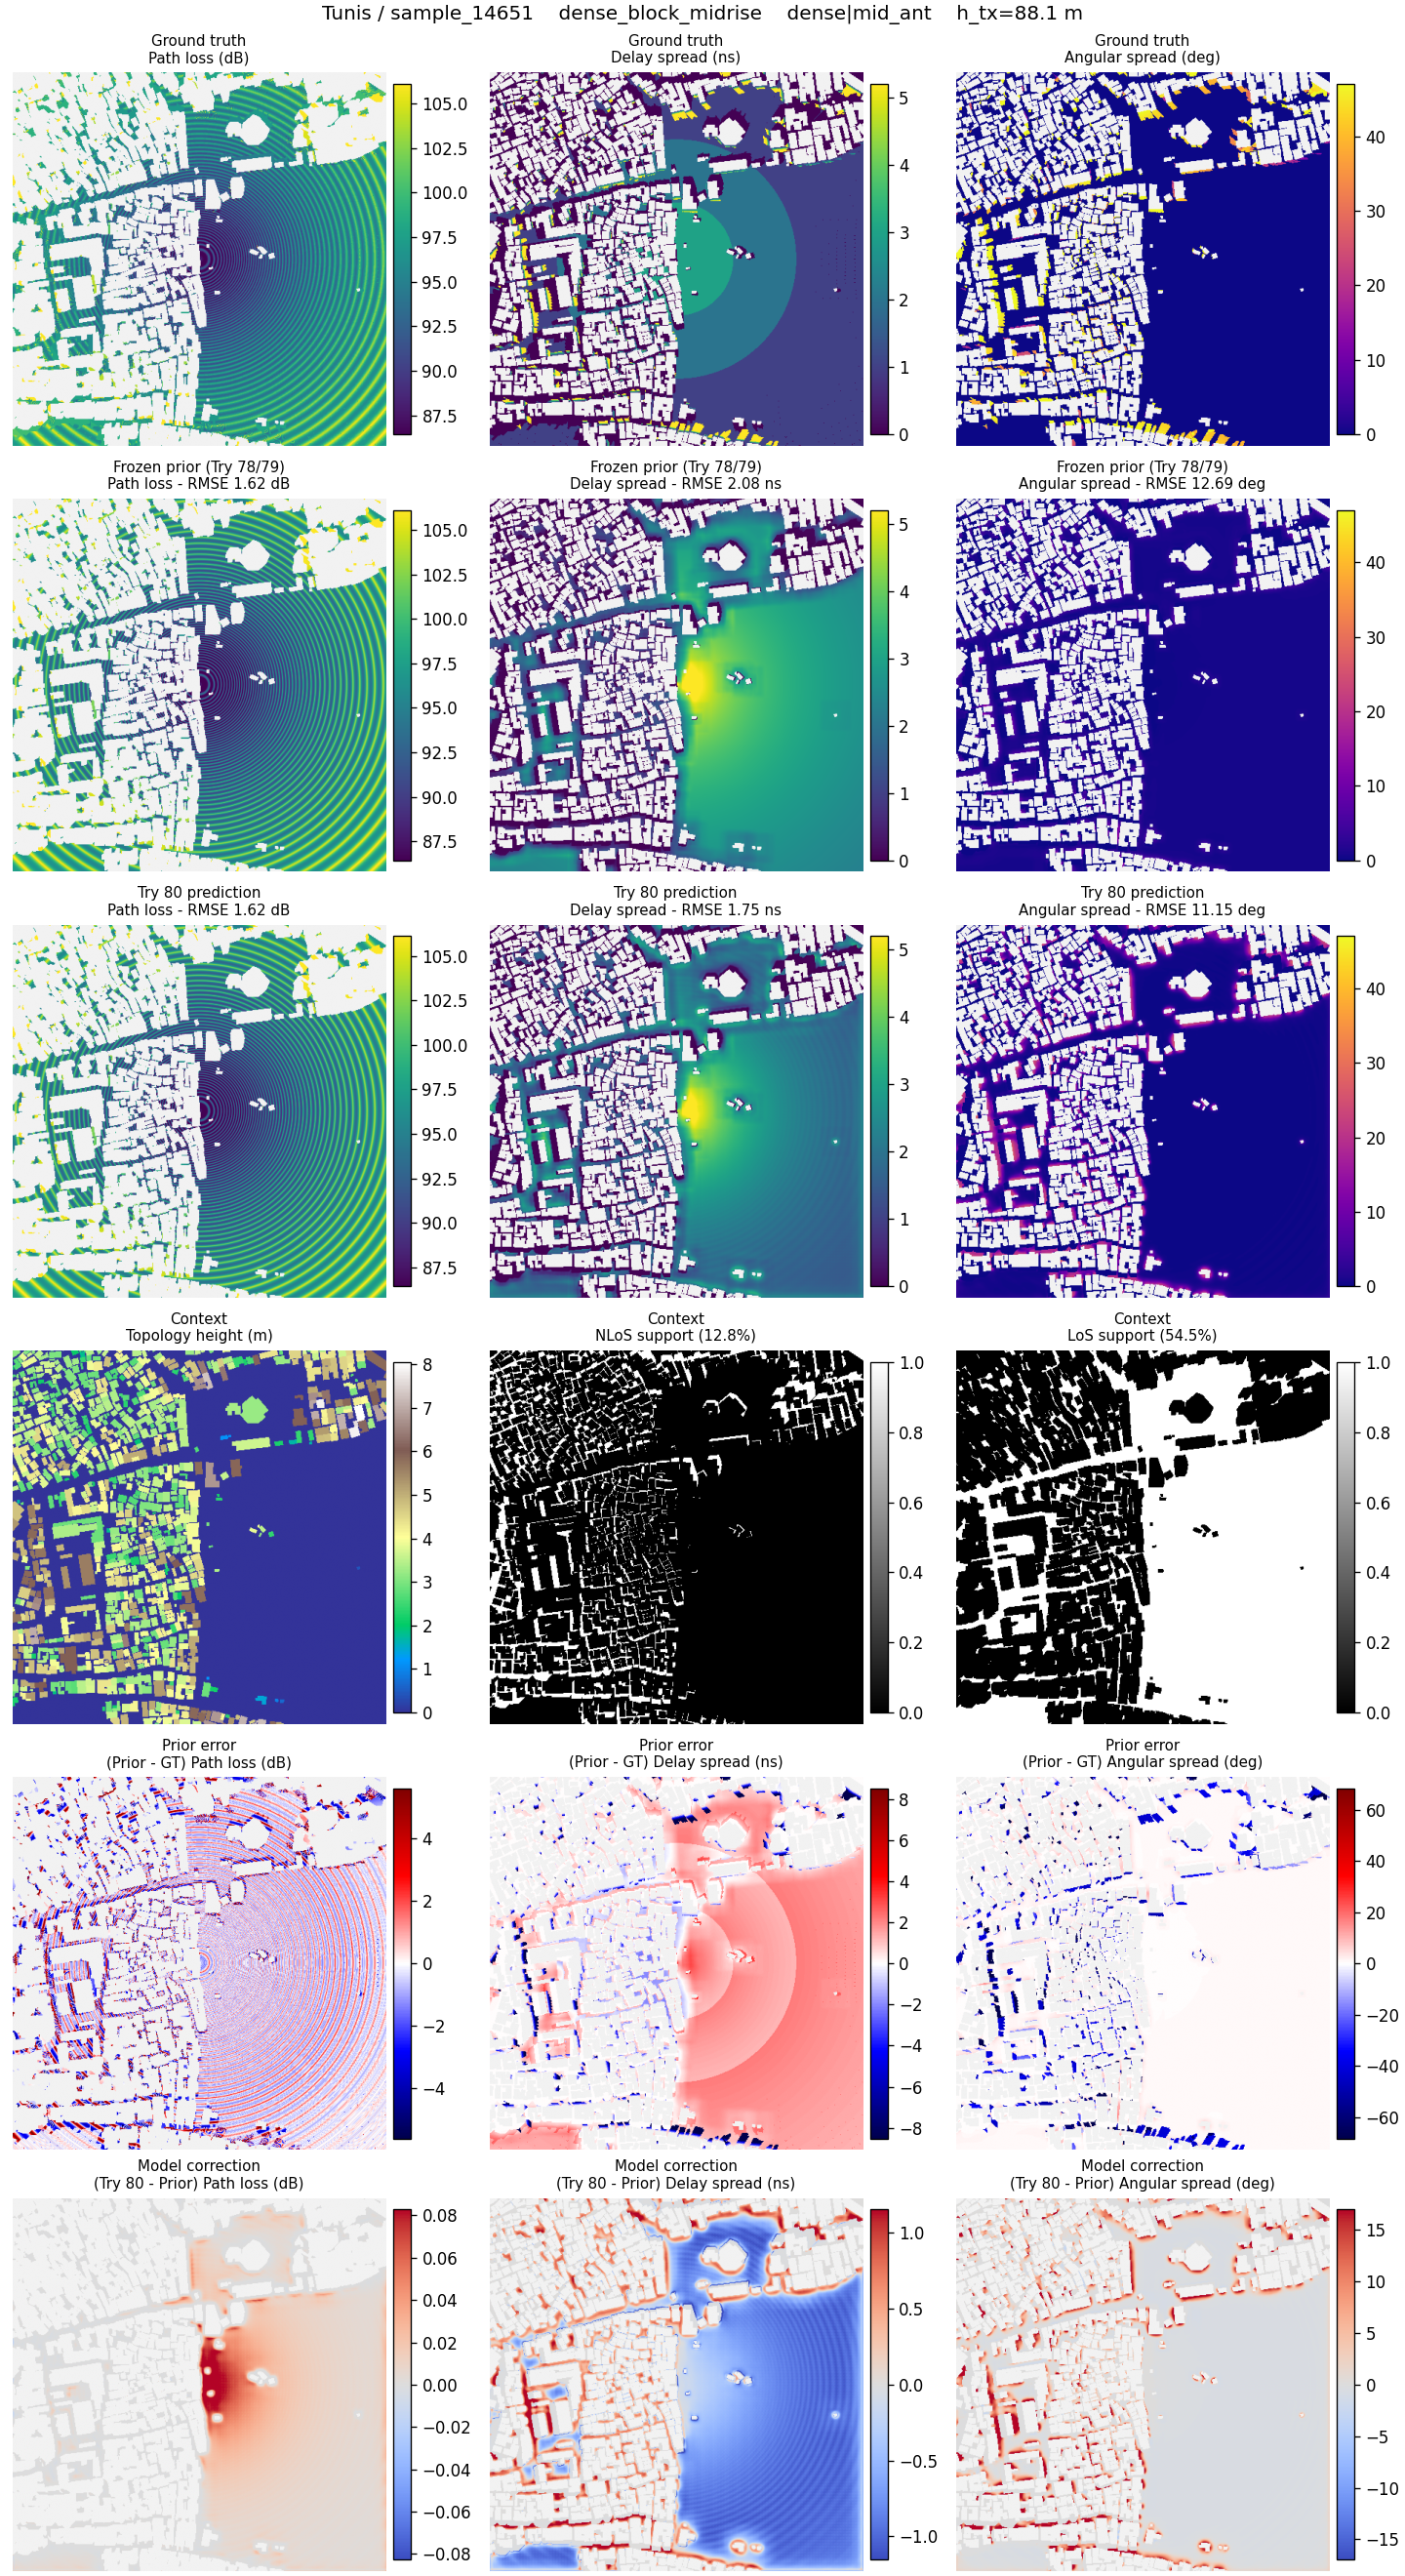
\includegraphics[width=\textwidth,height=0.88\textheight,keepaspectratio]{img/thesis_figures/try80_appendix_panels/try80_panel_dense_mid_ant_Tunis_sample_14651_6x3.png}
\caption[Representative final-model inspection panel.]%
{Representative final-model \(6\times3\) inspection panel for a dense,
mid-antenna validation diagnostic sample in Tunis. Columns: path loss, delay
spread, angular spread. Rows: ground truth, frozen prior, final
prediction, context / support mask, prior error
($\mathrm{Prior}-\mathrm{GT}$), and model correction
($\mathrm{Model}-\mathrm{Prior}$).}
\label{fig:try80_panel}
\end{figure}

The qualitative lesson from the path-loss prior is equally important: LoS path loss in this
dataset has a strong radial ring structure. Buildings explain visibility and
NLoS morphology, but in LoS they are not the main generator of the residual
shape. This is why a calibrated two-ray model could outperform many neural
iterations that tried to learn the same pattern from pixels alone.
